%%%%%%%%%%%%%%%%%%%%%%%%%%%%%%%%%%%%%%%%%%%%%%%%%%%%%%%%%%%%%%%%%%%%%%%%%%%%%%%%
%2345678901234567890123456789012345678901234567890123456789012345678901234567890
%        1         2         3         4         5         6         7         8

\documentclass[journal]{IEEEtranTIE}

% See the \addtolength command later in the file to balance the column lengths
% on the last page of the document

% The following packages can be found on http:\\www.ctan.org
%\usepackage{graphicx}
\usepackage{graphics} % for pdf, bitmapped graphics files
\usepackage{epsfig} % for postscript graphics files
\usepackage{subcaption}
\usepackage[noadjust]{cite}
%\usepackage{mathptmx} % assumes new font selection scheme installed
%\usepackage{times} % assumes new font selection scheme installed
\usepackage{algorithm,algpseudocode}
\usepackage{gensymb} % enable the use of degree symbol
\usepackage{amsmath,amssymb,amsfonts,amsthm} % assumes amsmath package installed
%\usepackage{booktabs}

% format for theorems etc.
\newtheorem{thm}{\bfseries Theorem}
\newtheorem{lem}{\bfseries Lemma}
\newtheorem{cor}{\bfseries Corollary}
\newtheorem{prop}{\bfseries Proposition}
\theoremstyle{remark}
\newtheorem{rem}{\bfseries Remark}
%\newtheorem*{proof*}{\bfseries Proof}

% format for argmin, argmax
\newcommand{\argmax}{\operatornamewithlimits{argmax}}

% format for cross-reference
\usepackage[capitalize]{cleveref}
\crefname{equation}{eq.}{eq.}
\Crefname{equation}{Eq.}{Eq.}
\crefname{thm}{theorem}{theorems}
\Crefname{thm}{Theorem}{Theorems}
\crefname{lem}{lemma}{lemmas}
\Crefname{lem}{Lemma}{Lemmas}
\crefname{cor}{corollary}{corollaries}
\Crefname{cor}{Corollary}{Corollaries}
\crefname{prop}{proposition}{propositions}
\Crefname{prop}{Proposition}{Propositions}
\crefname{rem}{remark}{remarks}
\Crefname{rem}{Remark}{Remarks}

%=====todonotes===== %
\usepackage{todonotes}
\usepackage{soul}
\definecolor{smoothgreen}{rgb}{0.7,1,0.7}
\sethlcolor{smoothgreen}

\newcommand{\todopara}[1]{\vspace{0px} %
	\todo[inline, color=black!10]{\textbf{[Paragraph:]} {#1}} %
}
\newcommand{\todonote}[1]{\vspace{0px} %
	\todo[inline, color=green!30]{\textbf{[Note:]} {#1}} %
}
\newcommand{\todoQ}[1]{\vspace{0px} %
	\todo[inline, color=orange!50]{\textbf{[Note:]} {#1}} %
}
\newcommand{\todohere}[1]{\hl{(\textbf{TODO:} #1)}}

\newcommand{\hidetodos}{
	\renewcommand{\todopara}[1]{}
	\renewcommand{\todonote}[1]{}
	\renewcommand{\todoQ}[1]{}
	\renewcommand{\todohere}[1]{}
	}

%---------- Macros for this paper
% random variables
\newcommand{\X}{X}
\newcommand{\Z}{Z}
\newcommand{\xg}{x^g}

\title{\LARGE \bf
	Measurement Dissemination-based Distributed Bayesian Filter using LIFO Exchange Protocol for Networked Unmanned Vehicles}
%Distributed Bayesian Filters for Multi-Vehicle Network by Using Latest-In-and-Full-Out Exchange Protocol of Observations}

\author{Chang Liu$^{1}$, Shengbo Eben Li$^{2}$ and J. Karl Hedrick$^{1}$% <-this % stops a space
\thanks{*The first two authors, C. Liu and S. Li, have equally contributed to this research. All correspondence should be addressed to S. Li. The work is supported by the ONR MURI project and the China National Science Foundation.
	}% <-this % stops a space
%\thanks{*This work is supported by the Embedded Humans: Provably Correct Decision Making for Networks of Humans and Unmanned Systems project, a MURI project funded by the Office of Naval Research and by the China National Science Foundation.}
\thanks{$^{1}$Chang Liu and J. Karl Hedrick are with the Vehicle Dynamics \& Control Lab, Department of Mechanical Engineering, University of California, Berkeley, Berkeley, CA 94709, USA. Email: {\tt\small changliu@berkeley.edu, khedrick@me.berkeley.edu}}%
\thanks{$^{2}$Shengbo Eben Li is with the Department of Automotive Engineering, Tsinghua University, Beijing, 100084, China. He has worked at the Department of Mechanical Engineering, University of California, Berkeley as a visiting scholar. Email: {\tt\small lisb04@gmail.com}}%
%\thanks{$^{3}$J. Karl Hedrick is with the Vehicle Dynamics \& Control Lab, Department of Mechanical Engineering, University of California, Berkeley, Berkeley, CA 94709, USA. Email: {\tt\small khedrick@me.berkeley.edu}}%
}

\begin{document}

%\hidetodos % hide all todos 

\maketitle
\thispagestyle{empty}
\pagestyle{empty}

%\setlength{\belowcaptionskip}{-10pt} % set the spacing between figure and text

%%%%%%%%%%%%%%%%%%%%%%%%%%%%%%%%%%%%%%%%%%%%%%%%%%%%%%%%%%%%%%%%%%%%%%%%%%%%%%%%
\begin{abstract}
This paper presents a measurement dissemination-based distributed Bayesian filtering (DBF) method for a network of unmanned ground vehicles (UGVs).
The DBF utilizes the Latest-In-and-Full-Out (LIFO) exchange protocol to disseminate the sensor measurements within local neighbors.
% for target search and tracking.
Different from existing statistics dissemination-based approaches that transmit posterior distributions or likelihood functions, each UGV under LIFO only exchanges 
%a communication buffer consisting of 
latest available measurements, 
%each UGV under LIFO only exchanges with neighboring UGVs a full communication buffer consisting of latest available measurements,
%receives the latest available measurements and then broadcasts full communication buffer to its neighborhood, 
which significantly reduces the transmission burden between each pair of UGVs to scale linearly with the network size.
Under the condition of fixed and undirected topology, LIFO can guarantee non-intermittent dissemination of all measurements over the network within finite time.
%, with each robot non-intermittently receiving measurements of all others.
Two types of LIFO-based DBF algorithms are then derived to estimate individual probability density function (PDF) for static target and moving target, respectively. 
For the former, each UGV locally fuses the newly received measurements while for the latter, a set of historical measurements is stored and sequentially fused. 
%Upon obtaining the latest available measurements of all robots, an iterative Bayesian filtering procedure is applied that alternates between prediction and updating steps. 
The consistency of LIFO-based DBF is proved that the estimated target position converges in probability to the true target position.
% when the number of measurements tends to infinity.
%the agreement between robots' estimated target position and the actual position.
The effectiveness of this method is demonstrated by simulation using heterogeneous sensors and by experiment using sonar sensors.
%by comparing with consensus-based distributed filters and a centralized filter in simulations of target localization.
\end{abstract}


%%%%%%%%%%%%%%%%%%%%%%%%%%%%%%%%%%%%%%%%%%%%%%%%%%%%%%%%%%%%%%%%%%%%%%%%%%%%%%%%
\section{INTRODUCTION}
Distributed filtering that focuses on using a group of networked UGVs to collectively infer environment status has been used for various applications, such as intruder detection \cite{chamberland2007wireless}, moving target tracking \cite{wang2012cooperative} and object localization \cite{song2012mobile}. 
Several techniques have been developed for distributed filtering.
For example, Olfati-Saber (2005) proposed a distributed Kalman filter (DKF) for estimating states of linear systems with Gaussian process and measurement noise \cite{2005distributed}.
Each DKF used low-pass and band-pass consensus filters to compute the average of weighted measurements and inverse-covariance matrices.
Madhavan et al. (2004) presented a distributed extended Kalman filter for nonlinear systems \cite{madhavan2004distributed}.
This filter was used to generate local terrain maps by using pose estimates to combine elevation gradient and vision-based depth with environmental features.
Gu (2007) proposed a distributed particle filter for Markovian target tracking over an undirected sensor network \cite{gu2007distributed}. 
Gaussian mixture models (GMM) were adopted to approximate the posterior distribution from weighted particles and the parameters of GMM were exchanged via average consensus filter.
As a generic filtering scheme for general system dynamics and arbitrary noise distributions, distributed Bayesian filters (DBF) have received increasing interest during past years \cite{bandyopadhyay2014distributed,julian2012distributed}, which is also the focus of this study.
It is worth noting that Bayesian filters can be reduced to Kalman filters and particle filters under appropriate conditions \cite{chen2003bayesian}.
%This study focuses on developing a distributed Bayesian filter (DBF) that is applicable for state estimation of general nonlinear systems and the proposed DBF is applied to search and tracking (SAT) of both static and moving targets.

The design of distributed filtering algorithms depends on the communication topology of multi-UGV network, which can be classified into two types: fusion center (FC)-based and neighborhood (NB)-based.
In the FC-based approaches, each UGV uses a filter to estimate local statistics of environment status based on its own measurement.
The local statistics is transmitted (possibly via multi-hopping) to a single FC, where a global posterior distribution (or statistical moments in DKF \cite{olfati2007consensus}) is calculated at each filtering cycle after receiving all local information \cite{zuo2006bandwidth,he2014networked}. %,vemula2006target
%At each filtering cycle, fusion center calculates the global state estimate only after receiving latest local estimates of all robots \cite{zuo2006bandwidth,vemula2006target}.
% has been a common structure for distributed filtering, in which local information collected by robots is transmitted (possibly via multi-hopping) to the fusion center for forming global estimation \cite{zuo2006bandwidth,ribeiro2006bandwidth}. 
%FC-based DBF is efficient for estimation in that it can collectively utilize all robots' information and thus useful for applications that only require information at a single central unit, such as in environmental monitoring.
%However, FC-based DBF requires constant communication link between each robot and the center, which is challenging for applications of robots in vast or complex areas.
In the NB-based approaches, a set of UGVs execute distributed filters to estimate individual posterior distribution. 
The consensus of individual estimates is achieved by solely communicating statistics and/or measurements within local neighbors.
%Only communication between neighboring agents is allowed.
The NB-based methods have become popular in recent years since such approaches do not require complex routing protocols and global network knowledge and therefore are rather robust to topological changes and link failures.
%, and thus suitable for networks with mobile agents.
%Besides, filtering is locally conducted on each robot, which requires less computation power compared to that in the fusion center.

%instead of communicating with a fusion center, each robot only exchanges information with neighboring robots and forms local estimation of the environment state. 
%NB-based DBF is advantageous over FC-based DBF in that no central unit is required, thus suitable for applications in which maintaining communication link between robots and center is challenging, such as in disaster situations.
%Besides, state estimation is locally conducted on each robot, which requires less computation power compared to that in the fusion center.

So far, most studies on NB-based distributed filtering have focused on the so-called \textit{statistics dissemination} strategy.
%that each UGV actually exchanges
This strategy directly exchanges environment statistics, including posterior distributions and likelihood functions, within neighboring UGVs \cite{hlinka2013distributed}.
%\todohere{concern: this categorization is based on Hlinka's survery. Will this cause trouble? Besides, the name statistics dissemination and measurement dissemination are also from this survey. Any issues?}
It can be further categorized into two types: leader-based and consensus-based. 
In the former, statistics is sequentially passed and updated along a path formed by active UGVs, called leaders.
Only the leaders can perform filtering based on its own and received measurements from local neighbors.
%\todohere{mention leader-based and consensus-based. 2 examples for leader-based and 3 examples for consensus-based.}
For example, Sheng et al. (2005) proposed a multiple leader-based distributed particle filter with Gaussian Mixer for target tracking \cite{sheng2005distributed}.
% to track multiple moving targets. 
Sensors are grouped into multiple uncorrelated cliques, in each of which a leader is assigned to perform particle filtering and exchanges particle information with other leaders.
%and the particle information is then exchanged among leaders.
%Distributed filters were run on a set of leader agents in uncorrelated sensor cliques and the particles were approximated as GMMs, the parameters of which were then exchanged among leaders for global estimation.
%In \cite{ram2007stochastic}, a circular topology that each sensor could only communicate with a fixed neighboring sensor was deployed for parameter estimation of a spatial field. 
%State estimates were updated using by sensors when passed along the circular topology Each sensor generates  based on that of the previous sensor and its own measurement and sequentially passes the estimate to its neighbor.
In the consensus-based distributed filters, every UGV diffuses environment statistics among neighbors, via which global agreement of the statistics is achieved by using multi-agent consensus laws \cite{olfati2007consensus,ren2005consensus,jadbabaie2003coordination}.
% by which all UGVs exchange statistics and executes consensus algorithms with neighbors, as proposed in , for fusion of statistics.
%For example, \todohere{find example on likelihood exchange} Julian et al. (2012) proposed a weighted-linear-average algorithm for fusing\todohere{find a more detailed word} posterior functions of environment status \cite{julian2012distributed}.
% consensus-based distributed particle filter (DPF) that uses linear average consensus approach for fusing posterior functions of environment status. .
For example, Hlinka et al. (2012) proposed a distributed method for computing an approximation of the joint (all-sensors) likelihood function by means of weighted-linear-average consensus algorithm when local likelihood functions belong to the exponential family of distributions \cite{hlinka2012likelihood}.
Saptarshi et al. (2014) presented a Bayesian consensus filter that uses logarithmic opinion pool for fusing posterior distributions of the tracked target \cite{bandyopadhyay2014distributed}. 
%The proposed BCF can incorporate non-Gaussian uncertainties and nonlinearity in target dynamic models and measurement models.  
%The DPF can work even when the network diameter, the maximum in/out degree, and the number of UGVs are unknown.
Other examples can be found in \cite{julian2012distributed} and \cite{beaudeau2012target}.
%There are other types of variants, for example, in \cite{ram2007stochastic}, a circular topology that each sensor can only communicate with a fixed neighboring sensor is deployed for parameter estimation of a spatial field. 
%Each sensor generates state estimate based on that of the previous sensor and its own measurement and sequentially passes the estimate to its neighbor.
%who using the incremental Robbins-Monro gradient algorithm locally at each sensor.

Despite the popularity of environment statistics dissemination strategy, exchanging statistics can consume high communication resources.
%Approximating statistics with parametric models, such as Gaussian Mixture Models \cite{sheng2005distributed}, can significantly reduce communication burden.
%However, such manipulation increases the computation burden for each UGV and sacrifices accuracy of filtering due to the approximation.
%which can be infeasible in vast area or complex environment.
% such as marine search, seismological rescue, etc. 
One promising remedy is to disseminate sensor measurement instead of environment statistics among neighbors.
%, which, however, has not been fully exploited.
% strategy has been developed for NB-based DBFs, by which raw or quantized measurements are exchanged among UGVs.
%This study focuses on the strategy of exchanging measurements in the neighborhood of each UGV, called the \textit{measurement dissemination-based} strategy, for the purpose of achieving a consensus of the probability density function (PDF) of the tracked target.  
One early work was done by Coates et al. (2004), which used adaptive encoding of sensor measurements to minimize communication overhead \cite{coates2004distributed}.
%Ribeiro et al. (2006) exchanged quantized measurements along with error-variance limits considering more pragmatic signal models \cite{ribeiro2006bandwidth}.
A recent study was conducted by Djuric et al. (2011), which proposed to broadcast raw measurements to other agents, and therefore each UGV had a complete set of measurements of other UGVs for executing particle filtering \cite{djuric2011non}. 
%At each time instant, a subset of UGVs that are in proximity of the tracked targets share their measurements for target position estimation.
% to all the remaining agents and apply local particle filter for target tracking 
%Another example can be found in \cite{rosencrantz2002decentralized}, in which both measurements and statistics were exchanged among sensors for distributed surveillance of the environment.
A shortcoming of aforementioned works is that their communication topologies are assumed to be a complete graph: 
even far from each other, each pair of UGVs should be directly connected by a unique edge, which is not always feasible in reality.
For incomplete graphs, Leung et al. (2010) explored a decentralized Extended Kalman filter for dynamic robot networks \cite{leung2010decentralized}.
The algorithm was shown to achieve centralized-equivalent filtering performance in simulations, but still lacked rigorous proofs on the estimation consistency.
% and consensus was provided. 


This paper presents a measurement dissemination-based distributed Bayesian filtering approach for target localization using networked UGVs.
% by introducing a Latest-In-and-Full-Out (LIFO) protocol.
% extends existing works by introducing a Latest-In-and-Full-Out (LIFO) protocol into distributed Bayesian filters (DBF) for networked UGVs. 
Each UGV only needs to broadcast the sensor measurements to its neighbors via single-hopping and then implements individual Bayesian filter locally after receiving transmitted measurements.
%The main benefit of using LIFO is on the reduction of communication burden, with the transmission data volume scaling linearly with the UGV number, 
%The LIFO significantly reduces the communication burden, 
The Latest-In-and-Full-Out (LIFO) protocol is introduced and can significantly reduces the communication burden, 
which scales the transmission data linearly with the UGV number, while a statistics dissemination-based strategy can suffer from the order of the environment size.
%In addition, LIFO spreads all UGVs' measurements among the network via multi-hopping, ensuring each UGV's access to all others' historical measurements.
%After receiving measurements from neighbors, each UGV runs Bayesian filter locally for environment state estimation. 
The proposed LIFO-based DBF has following properties:
(1)	For a fixed and undirected network, LIFO guarantees the global dissemination of measurements over the network in a non-intermittent manner.
%, with each UGV non-intermittently receiving (delayed) measurements of all other UGVs via local communication.
(2)	The corresponding DBF ensures the consistency of the estimated target position, i.e., the estimate converges in probability to the true value when the number of measurements tends to infinity.
%the estimated position converges in probability to the true target position when the number of measurements tends to infinity.
%, which also implies the consensus of target PDFs.
%which refers to the agreement between UGVs' estimates of target position and the true position of the target. 
%Moreover, consistency implies the consensus of UGVs' target PDFs.
%In this study, the consistency and consensus using LIFO-DBF is formally proved.

The rest of this paper is organized as follows: 
The problem of distributed Bayesian filtering is formulated in \cref{sec:prob_form}.
%The LIFO-based DBF algorithm is described in \cref{sec:LIFO-dbf}, followed by the proof of consistency and consensus in \cref{sec:consist_proof}.
The LIFO-based DBF algorithm is described in \cref{sec:LIFO-dbf}, followed by the proof of consistency in \cref{sec:consist_proof}.
Simulation and experiment results are presented in \cref{sec:sim} and \cref{sec:exp}.
The \cref{sec:conclu} concludes the paper.

\section{PROBLEM FORMULATION}\label{sec:prob_form}
Consider a network of $N$ UGVs to localize a target in a bounded two-dimensional space $S\in\mathbb{R}^{2}$. 
%The aim of UGVs is to localize a target in $S$. 
Each UGV is equipped with a sensor for environment perception. 
Due to the limit of communication range, each UGV can only share information 
with its local neighbors.
%locally by exchanging measurements with its neighbors. 
%The Bayesian filter is run on each UGV based on its own and received measurements to estimate the target position. %estimate true position of the target.
The Bayesian filter is run on each UGV based on its own measurements and the measurements of other UGVs to estimate the target position.

\subsection{Target and Sensor Model}
%Probabilistic Model of Binary Sensor}
%In this paper, distributed Bayesian filter is used to estimate the true target position by a network of binary sensors.
The target motion takes a deterministic discrete-time model: % that can be described by

\begin{equation}
\small
\label{eqn:tar_motion_model}
\xg_{k+1}=f(\xg_k), %,u^g_k),
%x_{k+1}=A_kx_k+B_ku^g_k+\epsilon,
\end{equation}\normalsize
where the superscript $g$ represents the target; $\xg_k\in S$ is the target position at time $k$. % and $u^g_k$ is the control input of the target.
%$A_k\in\mathbb{R}^{2\times 2},\;B_k\in\mathbb{R}^{2\times 2}$ and $\epsilon$ denotes the process noise.

%Each UGV constantly measures the target position and the 
The sensor measurement is described by a stochastic model:
\begin{equation}\label{eqn:meas_model}
z^i_k = h_i(\xg_k,x^i_k)+w^i_k,
\end{equation}
where the superscript $i\in\left\lbrace 1,\dots,N\right\rbrace$ represents the index of each UGV. $x^i_k\in S$ is the sensor position and $w^i_k$ is the white measurement noise.
% $x^i_k=[x^i_k;\theta^i_k]$ represents the sensor state, consisting of the sensor position $x^i_k$ and direction $\theta^i_k$.
The measurement function $h_i$ depends on the type of the sensor. 
%Let $\mathcal{F}(x^i_k)$ denote the sensor's sensing domain, 

%Due to the existence of measurement noise,
%A probabilistic sensor model, $P(z^i_k|x^g_k;x^i_k)$, that describes 
We are interested in the conditional probability of a certain measurement $z^i_k$ given the sensor and target state, which can be represented by $P(z^i_k|x^g_k;x^i_k)$ and is dependent on the distribution of the measurement noise.
This conditional probability is a key component for Bayesian filtering \cite{thrun2005probabilistic}.
%$P(z^i_k|x^g_k;x^i_k)$ relies on the distribution of the measurement noise. 
%For example, if 
%Usually, $w^i_k\sim\mathcal{N}(0,\Sigma^i_k)$ is a zero-mean Gaussian white noise and $P(z^i_k|x^g_k;x^i_k)$ can therefore be described as
For example, if $w^i_k\sim\mathcal{N}(0,\Sigma^i_k)$ is a zero-mean Gaussian white noise. Then, according to \Cref{eqn:meas_model}, $P(z^i_k|x^g_k;x^i_k)$ can be described as
%the probabilistic sensor model can be explicitly described as 
\footnote{For the purpose of simplicity, we will not explicitly write the parameter $x^{i}_k$ in $P(z^i_k|x^g_k;x^i_k)$ for the rest of the paper.}
\small\begin{equation*}%\label{eqn:prob_sensor3}
	P(z^i_k|x^g_k)=\mathcal{N}(h_i(\xg_k,x^i_k),\Sigma^i_k).
\end{equation*}\normalsize

The $h_i$ for several typical sensor are defined as follows \cite{bishop2010optimality}:

\textbf{Range-only sensors:} 
%when the target is within the sensor's sensing domain, 
the $h_i$ only depends on the relative Euclidean distance between the sensor and the target:
%\begin{subequations}
%	\begin{align}
\begin{equation*}%\label{eqn:ran_only}
	h_i(\xg_k,x^i_k)=\|\xg_k-x^i_k\|_2,
\end{equation*}	
%\begin{equation}\label{eqn:ran_only}
%h_i(\xg_k,w^i_k;x^i_k)=
%\begin{cases}
%\|\xg_k-x^i_k\|_2+w^i_k\; &\text{if}\, \xg_k\in\mathcal{F}(x^i_k)\\
%\emptyset\; &\text{if}\, \xg_k\notin\mathcal{F}(x^i_k)
%\end{cases},
%\end{equation}		
where $\|\cdot\|_2$ is the Euclidean distance in $S$.
%		w^i_k&\sim\mathcal{N}(0,\sigma^i),
%	\end{align}
%\end{subequations}

\textbf{Bearing-only sensors:} 
%when the target is within the sensor's sensing domain, 
the $h_i$ only depends on the relative bearing between the sensor and the target:
\begin{equation*}
	h_i(\xg_k,x^i_k)=\measuredangle (\xg_k-x^i_k),
\end{equation*}
%\begin{equation}
%h_i(\xg_k,w^i_k;x^i_k)=
%\begin{cases}
%\measuredangle (\xg_k-x^i_k)+w^i_k\; &\text{if}\, \xg_k\in\mathcal{F}(x^i_k)\\
%\emptyset\; &\text{if}\, \xg_k\notin\mathcal{F}(x^i_k)
%\end{cases},
%\end{equation}
where $\measuredangle$ denotes the angle from the sensor to the target.

\textbf{Range-bearing sensors:} the $h_i$ includes both the relative distance and bearing: % between the sensor and the target:
\begin{equation*}
	h_i(x^g_k,x^i_k)=x^g_k-x^i_k.
\end{equation*}
%\begin{equation}
%h_i(x_k,w^i_k;x^i_k)=
%\begin{cases}
%x_k-x^i_k+w^i_k\; &\text{if}\, x_k\in\mathcal{F}(x^i_k),\\
%\emptyset\; &\text{if}\, x_k\notin\mathcal{F}(x^i_k).
%\end{cases}
%\end{equation}

%the measurement by $i^\text{th}$ UGV is modeled as
%\begin{equation*}\small
%	z^i_k = 
%	\begin{cases}
%		1\qquad h^i(x_k;x^i_k)\geq \gamma\\
%		0 \qquad h^i(x_k;x^i_k) < \gamma
%	\end{cases},
%\end{equation*}\normalsize
%%\begin{equation*}\small
%%x^i_k=h^i(x_k;x^i_k),\; x_k\in S,
%%\end{equation*}\normalsize
%where $z^i_k$ denotes the measurement by $i^\text{th}$ sensor at time $k$; $h^i$ is the sensor property that characterizes the target position. 
%For example, $h^i$ can represent the power received by an ultrasonic sensor.
%When the received signal $x^i_k$ is greater than a threshold $\gamma$, indicating that the target is detected, the sensor returns $1$; otherwise, $0$ is returned by the sensor.
%%A binary sensor does not provide $x^i_k$ as its output. 
%%Instead, it only gives one of two possible values: $1$ when the signal $x^i_k$ is greater than a threshold $\gamma$, indicating the target is detected in the sensor's field of view; otherwise, $0$ is given by the sensor. Such model is shown below:
%%\begin{equation*}\small
%%z^i_k = 
%%\begin{cases}
%%1\qquad x^i_k\geq \gamma\\
%%0 \qquad x^i_k < \gamma
%%\end{cases},
%%\end{equation*}\normalsize
%%where $z^i_k$ denotes the measurement by $i^\text{th}$ sensor at time $k$.
%%The measurement of $i^\text{th}$ sensor at $k^\text{th}$ time step is denoted as $z^i_k$, the value of which follows a Bernoulli distribution.
%% and subjects to Bernoulli distribution $B(1,p_{i,k})$.

%A probabilistic sensor model, $P(z^i_k|x^g_k;x^i_k)$, that describes the conditional probability of a certain measurement $z^i_k$ given sensor and target state, is a key component for Bayesian filtering \cite{thrun2005probabilistic}.
%$P(z^i_k|x^g_k;x^i_k)$ relies on the distribution of the measurement noise. 


%We define a likelihood function to represent the probability that the target is detected by the sensor:

% as a function of the target and sensor positions:
%The following likelihood function gives the probability for $i^\text{th}$ sensor to obtain $z^i_k$:
%\small\begin{equation}\label{eqn:bin_sensor}
%	P(z^i_k|x_k;x^R_k)=p^{z^i_k}_{i,k}(1-p_{i,k})^{1-z^i_k},
%\end{equation}\normalsize
%where $p_{i,k}=P(z^i_k=1|x_k;x^R_k)$; $x_k$ and $x^R_k$ denote the target and UGV position at $k$, respectively.
%\small\begin{equation}\label{eqn:prob_sensor1}
%p^i_{1,k}=P(\Z^i_k\neq\emptyset|\xg_k;x^i_k)\in \left[0,1\right],\; \xg_k\in S,
%\end{equation}\normalsize
%where $\Z^i_k$ is a random variable denoting the possible measurement result; $x^i_k$ denotes the $i^\text{th}$ sensor's position.
%%; $X^g$ represents the set of all possible target positions.
%Correspondingly, the likelihood function for no target being detected is:
%\small\begin{equation}\label{eqn:prob_sensor0}
%p^i_{0,k}=P(\Z^i_k=\emptyset|\xg_k;y^{i}_k)=1-p^i_{1,k}.
%\end{equation}\normalsize
%%\Cref{eqn:bin_sensor} actually defines a binary sensor model parameterized by $x_k$ and $x^R_k$.

%The combination of \Cref{eqn:prob_sensor1,eqn:prob_sensor0} forms the probabilistic model for a sensor.


%\begin{equation}\label{eqn:prob_sensor3}
%	P(z^i_k|x^g_k)=\mathcal{N}(\bar{z}^i_k,\Sigma^i_k),
%\end{equation}
%\begin{equation}\label{eqn:prob_sensor3}
%	p^i_{1,k}=%\sim
%	\begin{cases}
%		\mathcal{N}(\bar{z}^i_k,\Sigma^i_k) & \text{if}\,\xg_k\in\mathcal{F}(x^i_k)\\
%		0 & \text{if}\,\xg_k\in\mathcal{F}(x^i_k)
%	\end{cases},
%\end{equation}
%where $\bar{z}^i_k$ is the nominal value of the measurement and equals $\|\xg_k-x^i_k\|$, $\measuredangle(\xg_k-x^i_k)$ and $\xg_k-x^i_k$ for range-only, bearing-only and range-bearing sensors, respectively. %$x_k-x^i_k$  and range-bearing

%Consequently,
%\begin{equation}\label{eqn:prob_sensor4}
%p^i_{0,k}=
%\begin{cases}
%0 & \text{if}\,\xg_k\in\mathcal{F}(x^i_k)\\
%1 & \text{if}\,\xg_k\in\mathcal{F}(x^i_k)
%\end{cases}.
%\end{equation}
%, and the measurement follows a Bernoulli distribution $B(1,p^i_{1,k})$, i.e.
%\small\begin{equation*}
%P(z^i_k|x;x^i_k)=(p^i_{1,k})^{z^i_k}(p^i_{0,k})^{1-z^j_l}.
%\end{equation*}\normalsize
% parameterized by $x_k$ and $x^i_k$. 
%For the purpose of simplicity, we will not explicitly write $y^{i}_k$ in the probabilistic sensor model for the rest of the paper.
%, with which all measurements are generated. 

%%\begin{rem}
%The commonly used likelihood functions for binary sensors include Gaussian function \cite{bonnie2012modelling,liu2015model} and step function \cite{djuric2008target}. For example, a Guassian function sensor model is defined as
%\small\begin{equation}\label{eqn:gauss_sensor}
%	p^i_{1,k}=e^{-\frac{1}{2}(x_k^g-x_k^i)^T{\Sigma}^{-1}(x_k^g-x_k^i)},
%\end{equation}\normalsize
%where $\Sigma$ is a positive definite covariance matrix characterizing the sensoring range and uncertainty.

%\small\begin{subequations}\label{eqn:gauss_sensor}
%	\begin{align}
%	p^i_{1,k}&=e^{-\frac{1}{2}(x_k^g-x_k^i)^T{\Sigma}^{-1}(x_k^g-x_k^i)}\\
%	%		\exp\left\lbrace -\frac{1}{2}(x-x^R)^T{\Sigma}^{-1}(x-x^R)\right\rbrace \\
%	p^i_{0,k}&=1-p^i_{1,k}.
%	\end{align}
%\end{subequations}\normalsize
%\end{rem}

\begin{rem}
	Given the knowledge of current target and UGV positions, current measurement by each UGV can be considered conditionally independent from its own past measurements and those by other UGVs \cite{bourgault2003optimal}.
\end{rem}

%\begin{rem} 
%	The proposed LIFO protocol to be described in \cref{sec:LIFO-dbf} and the consistency property proved in \Cref{sec:consist_proof} are applicable for general sensors, not limited to the ones described in this section. 
%	In addition, they also do not rely on the Gaussian noise assumption.
%	both homogeneous and heterogeneous binary sensors. 
%	A homogeneous model can simplify the analysis of completeness, while a heterogeneous model is closer to real sensing characteristics.
%	In addition, it also works for other types of sensors, such as laser scanners and cameras.
%\end{rem}

\subsection{Graphical Model of Communication Topology}
The UGV network is assumed to be connected, i.e., there exists a path, either direct or indirect, between every pair of UGVs.
Under this assumption, consider an undirected and fixed graph $G=(V,E)$, where $V=\left\lbrace 1,\dots,N\right\rbrace $ represents the index set of UGVs and $E=V\times V$ denotes the edge set. 
The adjacency matrix $A=\left[ A_{(ij)}\right] $ describes the communication topology of $G$:
\small\begin{equation*}
A_{(ij)}=\begin{cases}
1& \text{if}\;\left(i,j\right)\in E\\
0& \text{if}\;\left(i,j\right)\notin E
\end{cases},
\end{equation*} \normalsize
where $A_{(ij)}$ denotes the entity of the adjacency matrix. 
The notation $A_{(ij)}=1$ indicates that a communication link exists between $i^\text{th}$ and $j^\text{th}$ UGV and $A_{(ij)}=0$ indicates no direct communication between them.

The \textit{direct neighborhood} of $i^\text{th}$ UGV is defined as $\mathcal{N}_i=\left\lbrace j|A_{(ij)}=1,\forall j\in\left\lbrace1,\dots,N \right\rbrace \setminus \left\lbrace i \right\rbrace\right\rbrace $. 
All the UGVs in $\mathcal{N}_i$ can directly exchange information with $i^\text{th}$ UGV via single hopping. %in one step (single-hopping). 
%In addition to direct neighborhood, another set called \textit{available neighborhood} is defined as $\mathcal{Q}_i$, which contains indices of UGVs whose measurements can be received by the $i^\text{th}$ UGV given a specific measurement exchange protocol. 
We also define another set $\mathcal{Q}_i$, called \textit{available neighborhood}, that contains indices of UGVs whose measurements can be received by the $i^\text{th}$ UGV via single or multiple hoppings. %within single or multiple steps.
%given a specific measurement exchange protocol.
Therefore $\mathcal{N}_i\subseteq\mathcal{Q}_i$.
%but when only single-hopping is allowed, $\mathcal{N}_i=\mathcal{Q}_i$. 
%Some typical undirected and connected topologies include ring \cite{lawton2003decentralized}, line \cite{liu2010simple}, and star \cite{thatte2008sensor}.
\cref{fig:com_topo} illustrates three types of typical undirected and connected topologies: ring \cite{lawton2003decentralized}, line \cite{liu2010simple}, and star \cite{thatte2008sensor}. 
%All of them are undirected and connected topologies.

\begin{figure}%[thpb]
	\centering
	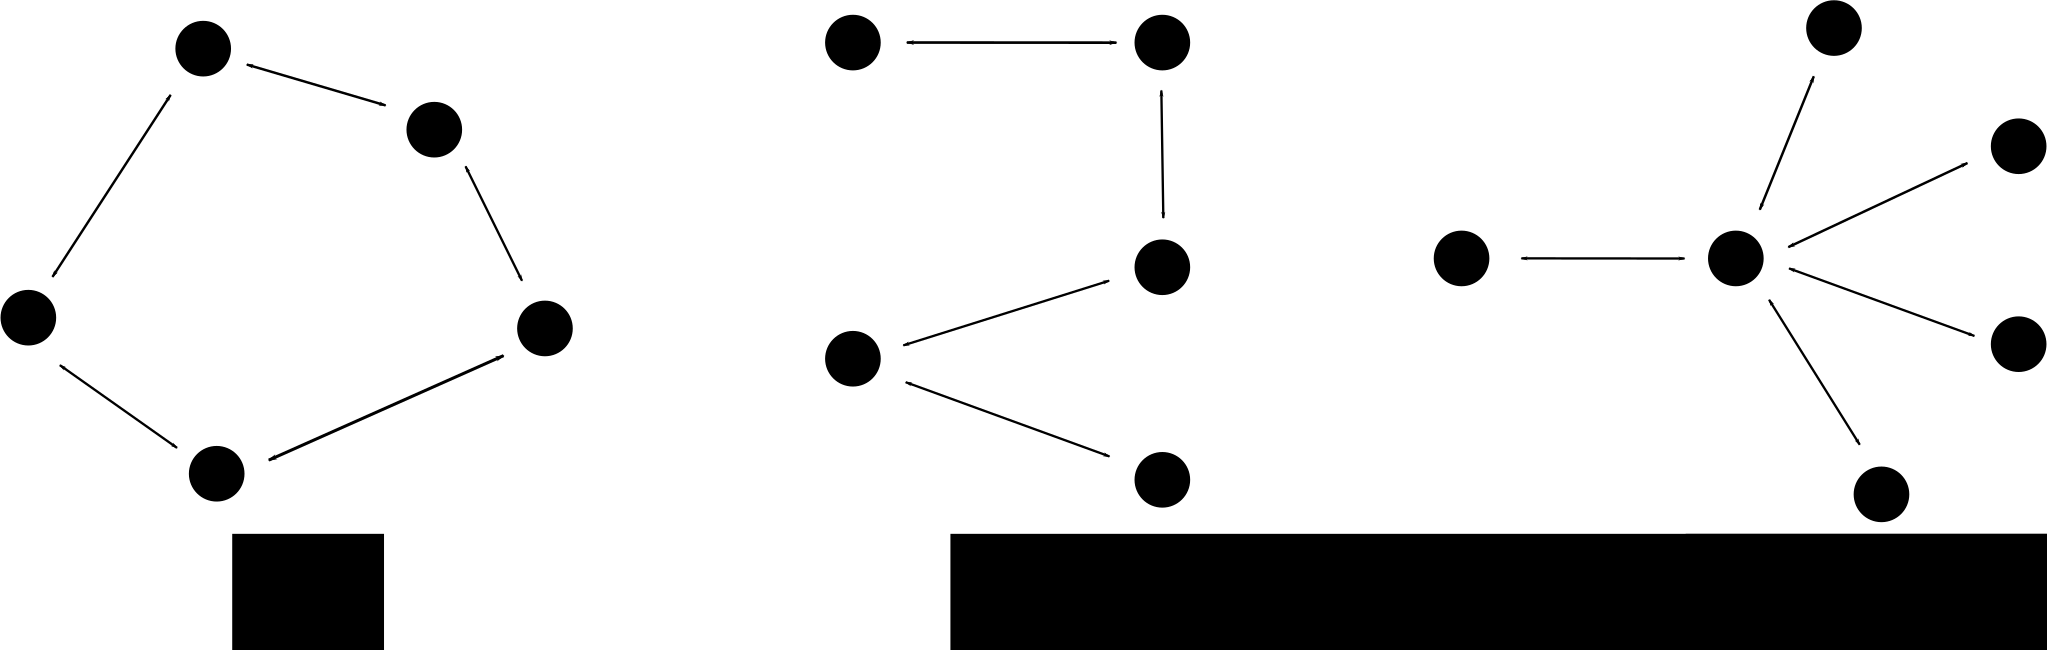
\includegraphics[width=0.45\textwidth]{figures/com_topo_new}
	\caption{Three types of topologies: (a) ring topology; (b) line topology; (c) star topology}
	\label{fig:com_topo}
\end{figure}

\subsection{Distributed Bayesian Filter for Multiple UGVs}\label{subsec:dbf}
The generic distributed Bayesian filter (DBF) is introduced in this section.
%, which is also stated in \cite{bandyopadhyay2014distributed} and \cite{julian2012distributed}. 
%Each UGV has its individual estimation of the probability density function (PDF) of target position, called \textit{individual PDF}. 
Let $\X_k\in S$ be the random variable that represents the position of the target at time $k$.
The probability density function (PDF) of $\X_k$, called \textit{individual PDF}, of $i^\text{th}$ UGV is then represented by
%=\left\lbrace z^i_1,\dots,z^i_k\right\rbrace
$P^i_{pdf}(\X_{k}|\mathbf{z}^i_{1:k})$, where $\mathbf{z}^i_{1:k}$ denotes the set of measurements by $i^\text{th}$ UGV and by UGVs in $\mathcal{Q}_i$, that have been received by $i^\text{th}$ UGV until time $k$.
%by UGVs in $\mathcal{Q}_i$ that have been transmitted to $i^\text{th}$ UGV by time $k$.
%from time $1$ through $k$ and $z^{\mathcal{Q}_i}_{1:k}$ means the set of measurements by UGVs in $\mathcal{Q}_i$ that are transmitted to $i^\text{th}$ UGV.
%Note that if the measurement by $j^\text{th}(j\in \mathcal{Q}_i)$ UGV at time $k'(k'\leq k)$ is not received by $i^\text{th}$ UGV, the corresponding element $z^j_{k'}$ in $z^{\mathcal{Q}_i}_{1:k}$ is empty and thus not utilized for computing $i^\text{th}$ individual PDF.
The initial individual PDF, $P^i_{pdf}(\X_0)$, is constructed %=P(\X_0) $P^i_{pdf}(\X_0|\mathbf{z}^i_0)$
%$P^i_{pdf}(x_0|z^i_0,z^{\mathcal{Q}_i}_0)=P(x_0)$, 
given all available prior information including past experience and environment knowledge. 
It is necessary to initialize the individual PDF such that the probability density of true target position is nonzero, i.e., $P^i_{pdf}(\X_0=x^g_0)\neq 0$. %$P^i_{pdf}(\X_0=x^g_0|\mathbf{z}^i_0)\neq 0$.

Under the framework of DBF, the individual PDF is recursively estimated by two steps: the prediction step and the updating step. 
%, based on measurements of $i^\text{th}$ UGV and UGVs in $\mathcal{Q}_i$.
 
\subsubsection{Prediction}
%The $i^\text{th}$ individual PDF at time $k-1$ is known, denoted as $P^i_{pdf}(x_{k-1}|z^i_{1:k-1},z^{\mathcal{Q}_i}_{1:k-1})$. 
%At time $k$, the prior individual PDF $P^i_{pdf}(x_{k-1}|z^i_{1:k-1},z^{\mathcal{Q}_i}_{1:k-1})$ is first predicted forward by using the Chapman-Kolmogorov equation:
At time $k$, the prior individual PDF $P^i_{pdf}(\X_{k-1}|\mathbf{z}^i_{1:k-1})$ is first predicted forward by using the Chapman-Kolmogorov equation:
%\small\begin{align}\label{eqn:bayes_pred}
%&P^i_{pdf}(x_k|z^i_{1:k-1},z^{\mathcal{Q}_i}_{1:k-1})\notag\\
%&=\int P(x_k|x_{k-1})P^i_{pdf}(x_{k-1}|z^i_{1:k-1},z^{\mathcal{Q}_i}_{1:k-1})dx_{k-1}
%\end{align}\normalsize
\small
\begin{equation}\label{eqn:bayes_pred}
P^i_{pdf}(\X_k|\mathbf{z}^i_{1:k-1})
=\int\limits_{\X_{k-1}\in S} P(\X_k|\X_{k-1})P^i_{pdf}(\X_{k-1}|\mathbf{z}^i_{1:k-1})d\X_{k-1},
\end{equation}\normalsize
where $P(\X_k|\X_{k-1})$ represents the state transition probability of the target, based on the Markovian motion model (\Cref{eqn:tar_motion_model}). % from the prior position $\X_{k-1}$ to the posterior position $\X_k$, 
% independent of UGV states. 
%This model describes 
%Note that the target is static in many search applications, such as the indoor search for stationary objects \cite{kulich2014single}. 
%, as defined in \Cref{eqn:tar_motion_model},
For the deterministic motion model, the state transition probability is simplified to be
\small\begin{equation}\label{eqn:markov_model}
P(\X_k=c_k|\X_{k-1}=c_{k-1})=\begin{cases}
1 & \text{if}\quad c_k=f(c_{k-1})\\ %,u^g_1
0 & \text{otherwise}
\end{cases}.
\end{equation}\normalsize
%and \Cref{eqn:bayes_pred} can be reduced to $P^i_{pdf}(x_{k}|z^i_{1:k-1},z^{\mathcal{Q}_i}_{1:k-1})=P^i_{pdf}(x_{k-1}|z^i_{1:k-1},z^{\mathcal{Q}_i}_{1:k-1})$.

\subsubsection{Updating}
The $i^\text{th}$ individual PDF is then updated by Bayes' theorem using the set of newly received measurements at time $k$, i.e., $\mathbf{z}^i_k$:
%\small\begin{align}\label{eqn:bayes_upd}
%&P^i_{pdf}(x_k|z^i_{1:k},z^{\mathcal{Q}_i}_{1:k})\notag\\
%&=K_iP^i_{pdf}(x_k|z^i_{1:k-1},z^{\mathcal{Q}_i}_{1:k-1})P(z^i_k|x_k)\prod\limits_{j\in\mathcal{Q}_i}P(z^j_k|x_k)
%\end{align}\normalsize
%\small\begin{equation}\label{eqn:bayes_upd}
%P^i_{pdf}(x_k|\mathbf{z}^i_{1:k})
%=K_iP^i_{pdf}(x_k|\mathbf{z}^i_{1:k-1})P(z^i_k|x_k)\prod\limits_{j\in\mathcal{Q}_i}P(z^j_k|x_k)
%\end{equation}\normalsize
\small\begin{equation}\label{eqn:bayes_upd}
P^i_{pdf}(\X_k|\mathbf{z}^i_{1:k})
=K_iP^i_{pdf}(\X_k|\mathbf{z}^i_{1:k-1})P(\mathbf{z}^i_k|\X_k),
\end{equation}\normalsize
where $P(\mathbf{z}^i_k|\X_k)$ comes from the sensor model and $K_i$ is a normalization factor, given by:
%\sma and l\begin{align*}
%K_i= and /\int P^i_{pdf}(x_k|z^i_{1:k-1},z^{\mathcal{Q}_i}_{1:k-1})P(z^i_k|x_k)\prod\limits_{j\in\mathcal{Q}_i}P(z^j_k|x_k)dx_k
%\end{align*}\normalsize
%\small\begin{align*}
%K_i=1/\int P^i_{pdf}(x_k|\mathbf{z}^i_{1:k-1})P(z^i_k|x_k)\prod\limits_{j\in\mathcal{Q}_i}P(z^j_k|x_k)dx_k
%\end{align*}\normalsize
\small\begin{align*}
K_i=\left[\int\limits_{\X_k\in S} P^i_{pdf}(\X_k|\mathbf{z}^i_{1:k-1})P(\mathbf{z}^i_k|\X_k)d\X_k\right]^{-1}.
\end{align*}\normalsize
%$P^i_{pdf}(\X_k|\mathbf{z}^i_{1:k})$ is the posterior individual PDF; 
% likelihood function of measurement $z^i_k$, as described in \Cref{eqn:prob_sensor3}.

\section{Distributed Bayesian Filter via Latest-In-and-Full-Out Protocol}\label{sec:LIFO-dbf}
This study proposes a Latest-In-and-Full-Out (LIFO) protocol for measurement exchange and derives corresponding distributed Bayesian filtering (DBF) algorithm, shorted as LIFO-DBF. 
The data communication in LIFO is synchronized with the execution of DBF.
In each step, LIFO only allows single-hopping communication within the direct neighborhood, but is able to broadcast measurements of each UGV to any other agent after a finite number of steps.
The individual PDF is forward predicted and updated in DBF after each LIFO cycle.
The theoretical analysis show that LIFO-DBF can ensure the consistency of distributed estimation while requiring much less communication burden than statistics dissemination-based methods. %and consensus


\subsection{Latest-In-and-Full-Out (LIFO) Protocol}\label{subsec:LIFO}
Under LIFO, each UGV contains a communication buffer (CB) to store its latest knowledge of measurements of all UGVs: 
\begin{equation*}
\mathbf{z}^{CB,i}_k=\left[ z^1_{k^i_1},\dots,z^N_{k^i_N},x^1_{k^i_1},\dots,x^N_{k^i_N}\right],
\end{equation*}
where $z^j_{k^i_j}$ represents the measurement made by ${j^\text{th}}$ UGV at time $k^i_j$ and $x^j_{k^i_j}$ denotes the sensor position when the associated measurement $z^j_{k^i_j}$ is made\footnote{ 
For the purpose of simplicity, we will not explicitly write $\left[x^1_{k^i_1},\dots,x^N_{k^i_N}\right]$ in $\mathbf{z}^{CB,i}_k$ for the rest of the paper.}.
At time $k$, $z^j_{k^i_j}$ is received and stored in ${i^\text{th}}$ UGV's CB, in which $k^i_j$ is the latest time of ${j^\text{th}}$ UGV's measurement that is available to ${i^\text{th}}$ UGV. Due to the communication delay, $k^i_j<k, \forall j\neq i$ and $k^i_i=k$ always hold.
The \textbf{LIFO protocol} is stated in \cref{alg:lifo}.
Note that under LIFO, $\mathcal{Q}_i=\left\lbrace 1,\dots,N\right\rbrace \setminus \left\lbrace i\right\rbrace$, which will be proved in \Cref{cor1}.
\cref{fig:LIFO} illustrates the LIFO cycles with 3 UGVs using a line topology. 
%Two facts can be noticed in \cref{fig:LIFO}: (1) all UGV CBs are filled within 3 steps, which means under LIFO each UGV has a maximum delay of 2 steps for receiving measurements from other UGVs; (2) after filled, CBs are updated non-intermittently, which means each UGV continuously receives new measurements of other UGVs. Extending the two facts to a network of $N$ UGVs, 
For general graphs, we have the following proposition:
\medskip
\begin{prop}\label{prop1}
%For a fixed and undirected network of $N$ UGVs, LIFO uses the shortest path(s) between $i^\text{th}$ and $j^\text{th}$ UGV to exchange measurement, the length of which is the delay $\tau_{i,j}$ between these two UGVs.
For a fixed and undirected network of $N$ UGVs, the latest measurements of $i^\text{th}$ and $j^\text{th}$ UGV are exchanged via the shortest path(s) under LIFO. The delay of exchange $\tau_{i,j}$ is equivalent to the length of the shortest path(s) between them.
\end{prop}

\begin{proof}
Since the network is connected, there exists a minimum integer $\tau_{i,j}$ such that $A^{\tau_{i,j}}_{(i,j)}>0$ and $\tau_{i,j}$ is the length of a shortest path between $i^\text{th}$ and $j^\text{th}$ UGV \cite{deo2016graph}. Under the LIFO, the latest measurement of $i^\text{th}$ UGV will always be propagated via the CBs of UGVs along a shortest path between $i^\text{th}$ and $j^\text{th}$ UGV. 
Therefore, the latest measurement that $j^\text{th}$ UGV receives from $i^\text{th}$ UGV is delayed by $\tau_{i,j}$ rounds of communication.
\end{proof}
%\begin{proof} 
%Without loss of generality, assume that there is a unique shortest path between $i$ and $j$, denoted by $T^{j,i}_{n^*}=\left(v_1,\dots,v_{n^*}\right)$, with $v_1=j,v_{n^*}=i,v_{m+1}\in\mathcal{N}_{v_m}$. 
%Then, the distance between $i$ and $j$ is $d(j,i)=n^*-1$. 
%The following mathematical induction will prove \Cref{prop1}.
%
%Step (1): When $d(j,i)=1$, $j\in\mathcal{N}_i$ and $j$ can directly send $z^j_k$ to $i$. Then $z^j_k$ is stored in $i^\text{th}$ CB at time $k+1$, i.e. $\tau_{i,j}=1$. 
%\Cref{prop1} holds for $d(j,i)=1,\,\forall i,j\in\left\lbrace 1,\dots,N\right\rbrace $.
%
%Step (2): Suppose that \Cref{prop1} holds for $d(j,i)=s,\,s\geq 2,\,\forall i,j\in\left\lbrace 1,\dots,N\right\rbrace$. 
%Then for $d(j,i)=s+1$, i.e., $n^*=s+2$, by the Bellman's principle of optimality, the path $T^{j,l}_{n^*-1}=\left(v_1,\dots,v_{n^*-1}\right)$ is a shortest path between $j$ and $l$, where $v_{n^*-1}=l$ and $i\in \mathcal{N}_l$. 
%The assumption that \Cref{prop1} holds for $d(j,i)=s$ implies that $z^j_k$ is received and stored in $l^\text{th}$ UGV's CB at time $k+s$. 
%Since $i\in\mathcal{N}_l$, $i^\text{th}$ UGV receives $z^j_k$ at $k+s+1$. 
%For any other path $T^{j,i}_{n}=\left(v_1,\dots,v_{n}\right)$ with $n>n^*$, $z^j_k$ cannot be received by $i$ earlier than $k+s+1$. 
%Therefore $\tau_{i,j}=s+1$. 
%This proves the \Cref{prop1} for $d(j,i)=s+1$.
%\end{proof}
%\vspace{\baselineskip}

\begin{algorithm}
	\caption{LIFO Protocol}
	\label{alg:lifo}
	\begin{algorithmic}
		\State \textbf{(1)} Initialization:
		The CB of $i^\text{th}$ UGV is initialized when $k=0$: 
		\begin{equation*}
		%$\begin{array}{c}
		z^j_{k^i_j}=\varnothing,\; k^i_j=0,\;j=1,\dots,N
		%\end{array}$\\
		\end{equation*}
		
		\State \textbf{(2)} At $k^\text{th}$ step for $i^\text{th}$ UGV :		
		\State (2.1) Receiving Step:
		
		The $i^\text{th}$ UGV receives all CBs of its direct neighborhood $\mathcal{N}_i$, each of which corresponds to the (k-1)-step CB of a UGV in $\mathcal{N}_i$. 
		%		The received CBs are totally $|\mathcal{N}_i|$ groups, each of which corresponds to the (k-1)-step CB of a UGV in $\mathcal{N}_i$. 
		The received CB from $l^\text{th}$ ($l\in \mathcal{N}_i$) UGV is denoted as
		\begin{equation*}
		\mathbf{z}^{CB,l}_{k-1}=\left[ z^1_{(k-1)^l_1},\dots,z^N_{(k-1)^l_N}\right],\; l\in\mathcal{N}_i
		\end{equation*}
		
		\State (2.2) Observation Step: 
		
		The $i^\text{th}$ UGV updates $z^j_{k^i_j}\,(j=i)$ by its own measurement at current step:
		\begin{equation*}
		z^j_{k^i_j}=z^i_k,\;k^i_j=k,\;\text{if }j=i.
		\end{equation*}
		
		\State (2.3) Comparison Step:
		
		The $i^\text{th}$ UGV updates other elements of its own CB, i.e., $z^j_{k^i_j}\,(j\neq i)$, by selecting the latest information among all received CBs from $\mathcal{N}_i$. For all $j\neq i$,
		\small\begin{align*}
		l_\text{latest}&=\argmax_{\left\lbrace l\in \mathcal{N}_i,\;i\right\rbrace}\left\lbrace\left(k-1\right)^i_j,\left(k-1\right)^l_j  \right\rbrace\\
		z^j_{k^i_j}&=z^j_{\left(k-1\right)^{l_\text{latest}}_j},\; k^i_j=\left(k-1\right)^{l_\text{latest}}_j
		\end{align*} \normalsize
		
		\State (2.4) Sending Step:
		
		The $i^\text{th}$ UGV broadcasts its updated CB to all of its neighbors defined in $\mathcal{N}_i$.
		%\bottomrule
		%\end{tabular}
		
		\State \textbf{(3)} $k\leftarrow k+1$ until stop %$\hfill\blacksquare$
	\end{algorithmic}
\end{algorithm}

%\medskip
\begin{cor}\label{cor1}
For the same topology assumption in \Cref{prop1}, all elements in $\mathbf{z}^{CB,i}_k$ under LIFO become nonempty when $k\geq N$. 
This implies $\mathcal{Q}_i = \left\lbrace1,\dots,N \right\rbrace \setminus \left\lbrace i\right\rbrace $.	
\end{cor}
%\begin{proof}
%In a network of $N$ UGVs, the maximal length of shortest paths is no greater than $N-1$. Based on \Cref{prop1}, $\tau_{i,j}\leq N-1$ and thus all elements of $\mathbf{z}^{CB,i}_k$ become filled when $k\geq N$.
%\end{proof}

%\medskip
\begin{cor}\label{cor2}
For the same topology assumption in \Cref{prop1}, once elements in $\mathbf{z}^{CB,i}_k$ are nonempty, the updating of each element is non-intermittent. Moreover, $k-N<k^i_j\leq k$.
\end{cor}
%\begin{proof}
%For a network with fixed topology, shortest path(s) between any pair of nodes are fixed. 
%Therefore, based on \Cref{prop1}, $\tau_{i,j}$ is constant and the updating of each element in $\mathbf{z}^{CB,i}_k$ is non-intermittent.
%\end{proof}
\medskip
%\begin{rem}
	Compared to statistics dissemination, LIFO is generally more communication-efficient for distributed filtering. 
	To be specific, assume the environment $S$ is represented by an $M\times M$ grid.
%	To be specific, consider an $M\times M$ environment with 
	For a network of $N$ UGVs, the transmitted data of LIFO between each pair of UGVs are only the CB of each UGV and the corresponding sensor states, the size of which is $O(N)$, scaling linearly with UGV number. 
	On the contrary, the transmitted data for a statistics dissemination approach that transmits unparameterized posterior distributions or likelihood functions is $O(M^2)$, which is in the order of the environment size. 
	Since $M$ is generally much larger than $N$ in applications such as target localization and environment exploration, LIFO requires much less communication resources.
%\end{rem}

\begin{figure}%[thpb]
	\centering
	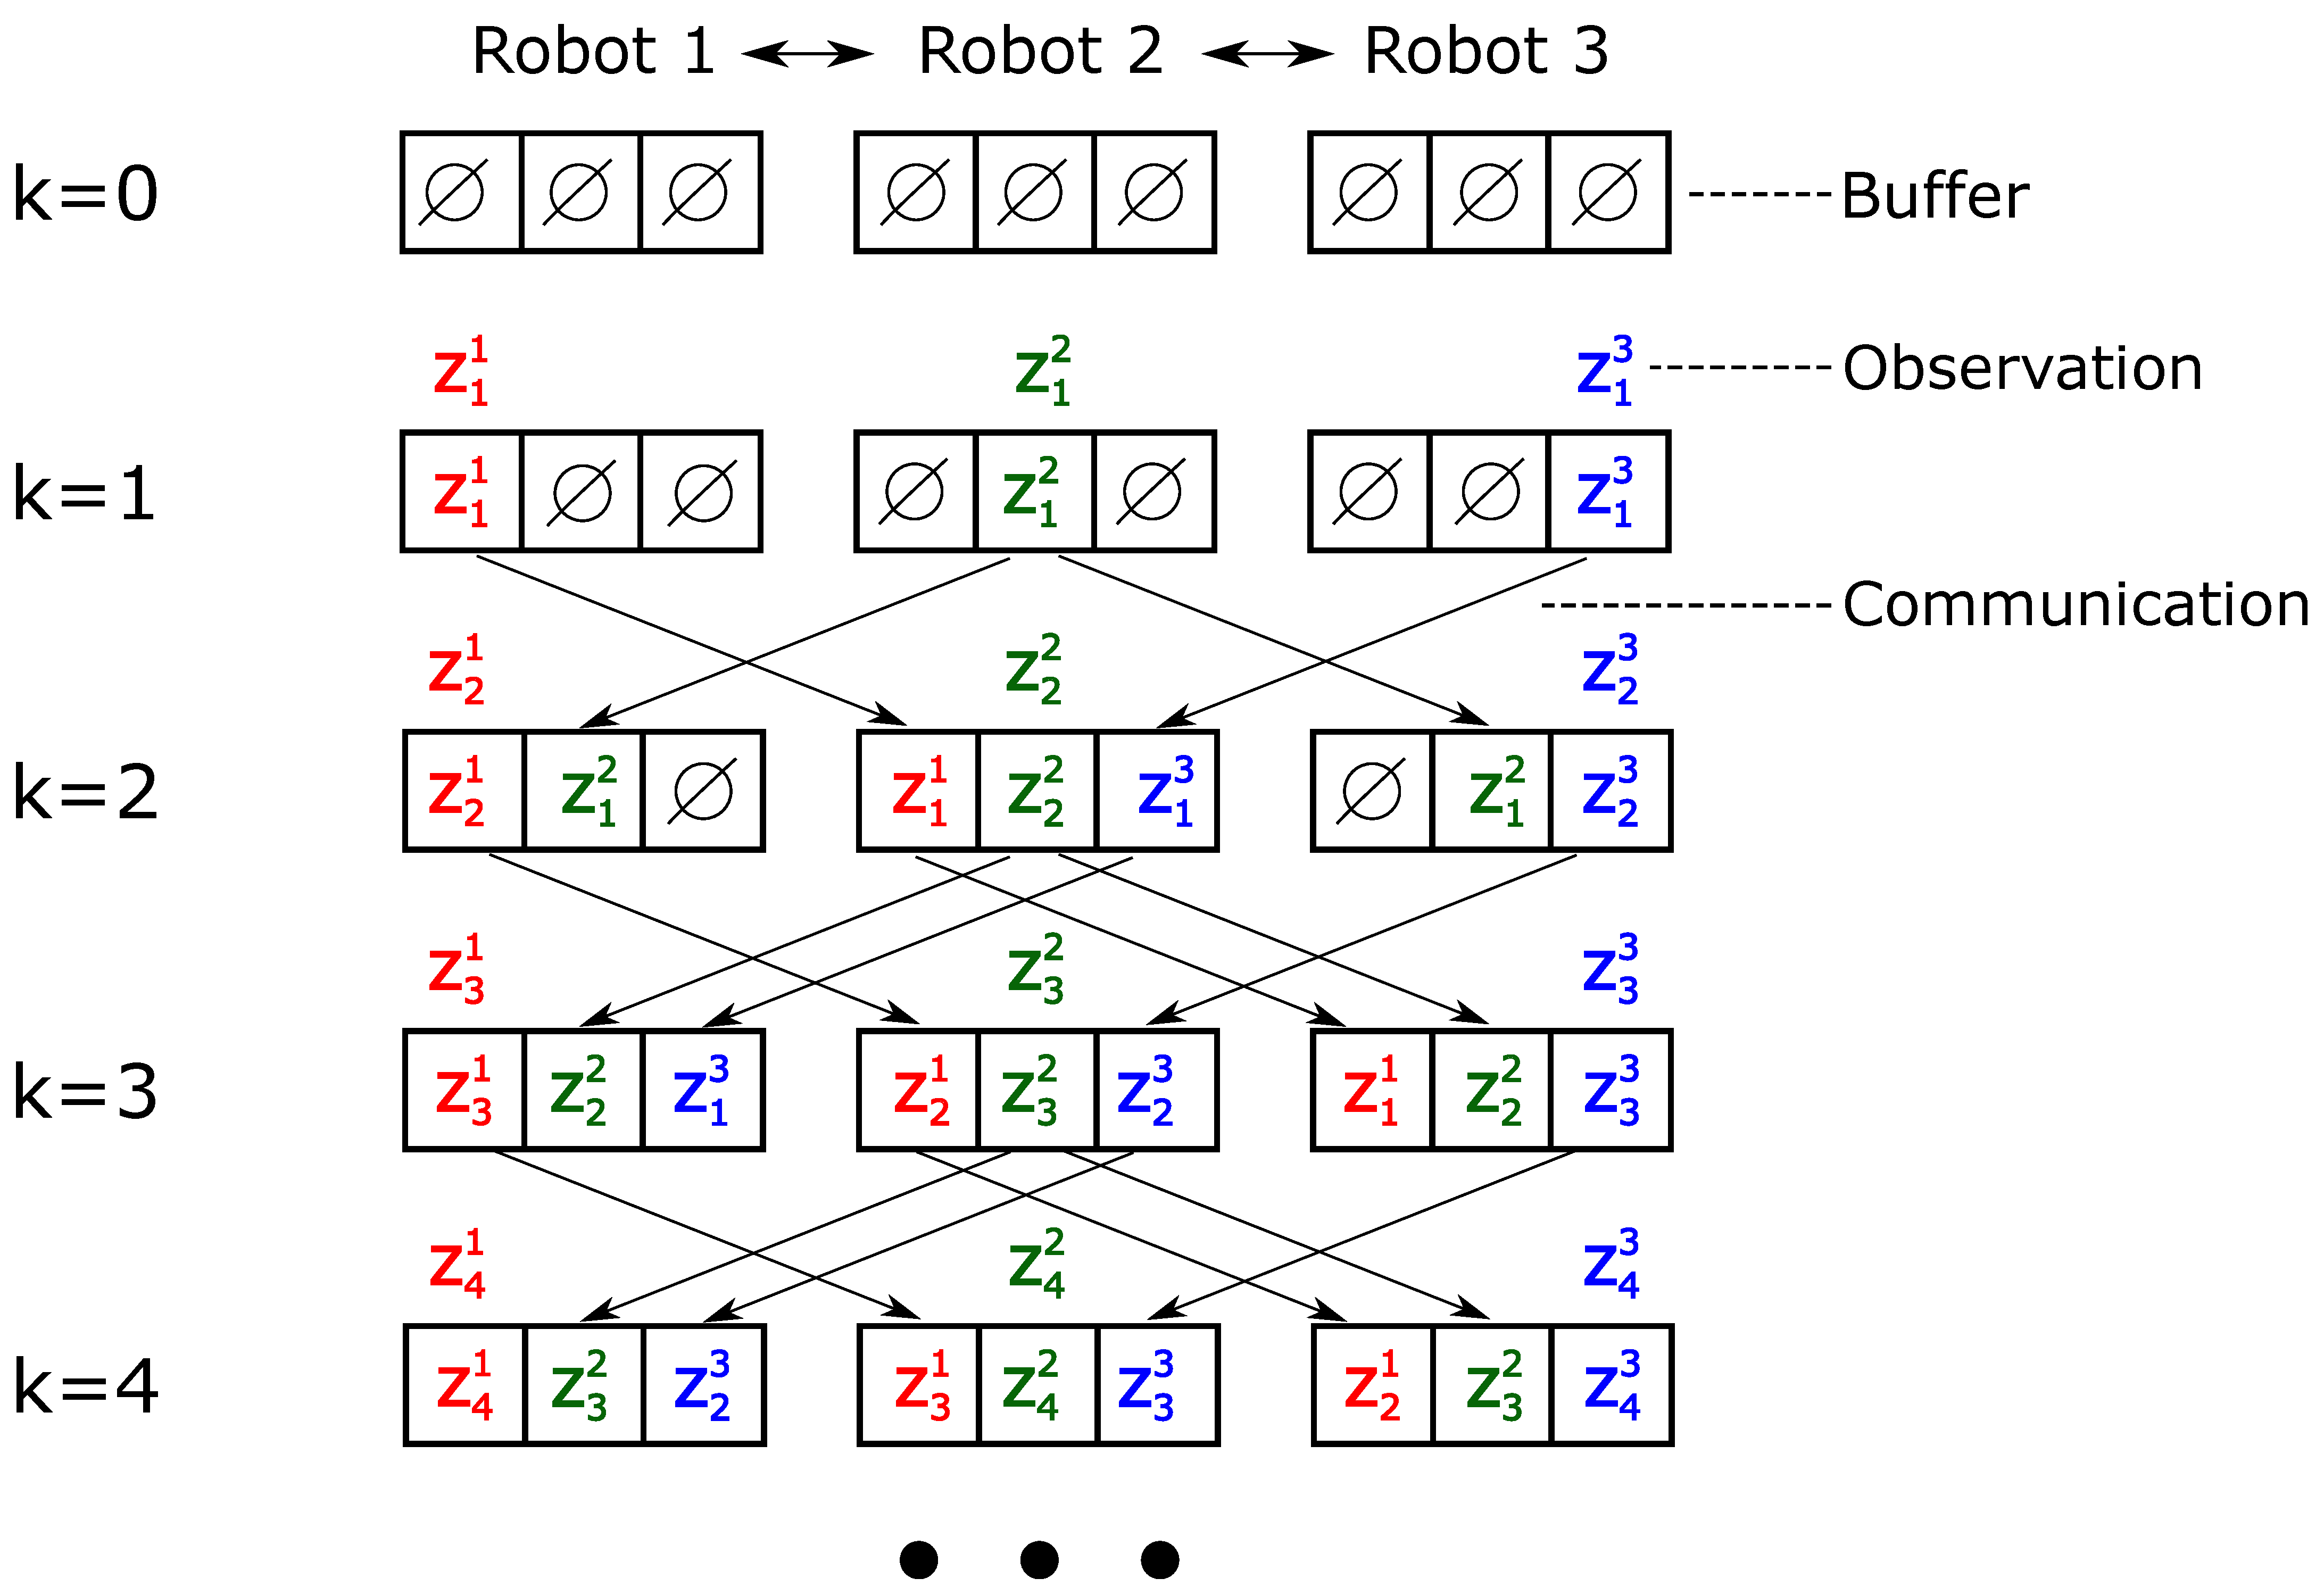
\includegraphics[width=0.48\textwidth]{figures/data_exchange}
	\caption{Example of LIFO with three UGVs using line communication topology. In this case,  $\mathcal{N}_1=\left\lbrace 2 \right\rbrace,\,\mathcal{Q}_1=\left\lbrace 2,3 \right\rbrace;\: \mathcal{N}_2=\left\lbrace 1,3 \right\rbrace,\,\mathcal{Q}_2=\left\lbrace 1,3 \right\rbrace;\: \mathcal{N}_3=\left\lbrace 2 \right\rbrace,\,\mathcal{Q}_3=\left\lbrace 1,2 \right\rbrace$.}
	\label{fig:LIFO}
\end{figure}

\subsection{Algorithm of LIFO-DBF for Static Target}\label{subsec:LIFO-dbf-sta-tar} 

This section derives the LIFO-DBF algorithm for localizing a static target. 
It is assumed that all UGVs know the sensor model of other UGVs.
%Each UGV locally stores last-step individual PDF, i.e., $P^i_{pdf}(x|\mathbf{z}^{i}_{1:k-1})$. 
%According to \Cref{cor2}, $\mathbf{z}^i_k=\mathbf{z}^{CB,i}_k$ and $\mathbf{z}^{i}_{1:k}=\mathbf{z}^{CB,i}_{1:k}=\left[ z^1_{1:k^i_1},\dots,z^N_{1:k^i_N}\right]$.
According to \Cref{cor2}, $\mathbf{z}^i_k$ and $\mathbf{z}^{i}_{1:k}$ in \Cref{eqn:bayes_upd} equals $\mathbf{z}^{CB,i}_k$ and $\mathbf{z}^{CB,i}_{1:k}$, respectively.
The assumption of static target can simplify the Bayesian filter as the prediction step becomes trivial. 
At time $k$, the $i^\text{th}$ UGV starts from the last-step individual PDF that is locally stored, i.e., $P^i_{pdf}(\X|\mathbf{z}^{i}_{1:k-1})$\footnote{Since the target is static, we drop the subscript $k$ in $\X_k$.}. 
The $i^\text{th}$ individual PDF is then updated by fusing all measurements in $\mathbf{z}^i_k$:
\small\begin{align*}\label{eqn:LIFO-dbf-sta-tar}
P^i_{pdf}(\X|\mathbf{z}^{i}_{1:k})&=K_iP^i_{pdf}(\X|\mathbf{z}^i_{1:k-1})P(\mathbf{z}^i_k|\X)\notag\\
&=K_iP^i_{pdf}(\X|\mathbf{z}^{i}_{1:k-1})\prod\limits_{j=1}^{N}P(z^j_{k^i_j}|\X),
\end{align*}\normalsize

%\small\begin{equation}\label{eqn:LIFO-dbf-sta-tar}
%P^i_{pdf}(x|\mathbf{z}^{i}_{1:k})=K_iP^i_{pdf}(x|\mathbf{z}^{i}_{1:k-1})\prod\limits_{j=1}^{N}P(z^j_{k^i_j}|x)
%\end{equation}\normalsize
where
\small\begin{equation*}
K_i=\left[\int\limits_{\X\in S} P^i_{pdf}(\X|\mathbf{z}^{i}_{1:k-1})\prod\limits_{j=1}^{N}P(z^j_{k^i_j}|\X)d\X\right]^{-1}.
\end{equation*}\normalsize

\subsection{Algorithm of LIFO-DBF for Moving Target}\label{subsec:LIFO-dbf-mov-tar}
This section derives the LIFO-DBF for localizing a moving target. 
Instead of storing last-step PDF, at time $k$ each UGV maintains an individual PDF of time $(k-N)$ and a collection of historical measurements, called the \textit{record set}, from time $(k-N+1)$ to $k$. 
The $i^\text{th}$ individual PDF is then alternatively predicted and updated by using the aforementioned Bayesian filter (\Cref{eqn:bayes_pred,eqn:bayes_upd}) from $(k-N)$ to $k$ to obtain $P^i_{pdf}(\X_k|\mathbf{z}^{i}_{1:k})$.

\cref{fig:LIFO-DBF} illustrates the LIFO-DBF procedure for the $1^\text{st}$ UGV as an example \footnote{Due to the space limit, in this figure we use $P^i_{pdf}(k)$, $P^i_{pdf}(k-N)$ and $P^i_{pdf}(k-N+1)$ to represent $P^i_{pdf}(\X|\mathbf{z}^{i}_{1:k})$ $P^i_{pdf}(\X|\mathbf{z}^{i}_{1:k-N})$ and $P^i_{pdf}(\X|\mathbf{z}^{i}_{1:k-N+1})$, respectively.}.
%With a line topology, the record set of $1^\text{st}$ UGV is shown as a triangle.
% shape formed by squares that contain measurements from $(k-N+1)$ to $k$.
$\Omega^i_{\xi}\,\left(\xi=1,\dots,N\right) $ denote the index set of UGVs whose measurement at time $(k-N+\xi)$ is stored in $i^\text{th}$ UGV's record set, i.e. $\Omega^i_{\xi}=\left\lbrace j\in \mathcal{Q}_i \bigcup \left\lbrace i \right\rbrace | z^j_{k-N+\xi} \text{ is in the record set} \right\rbrace$.
The \textbf{LIFO-DBF algorithm} for moving target is stated in \cref{alg:lifo-dbf}.

\begin{figure}%[thpb]
	\centering
	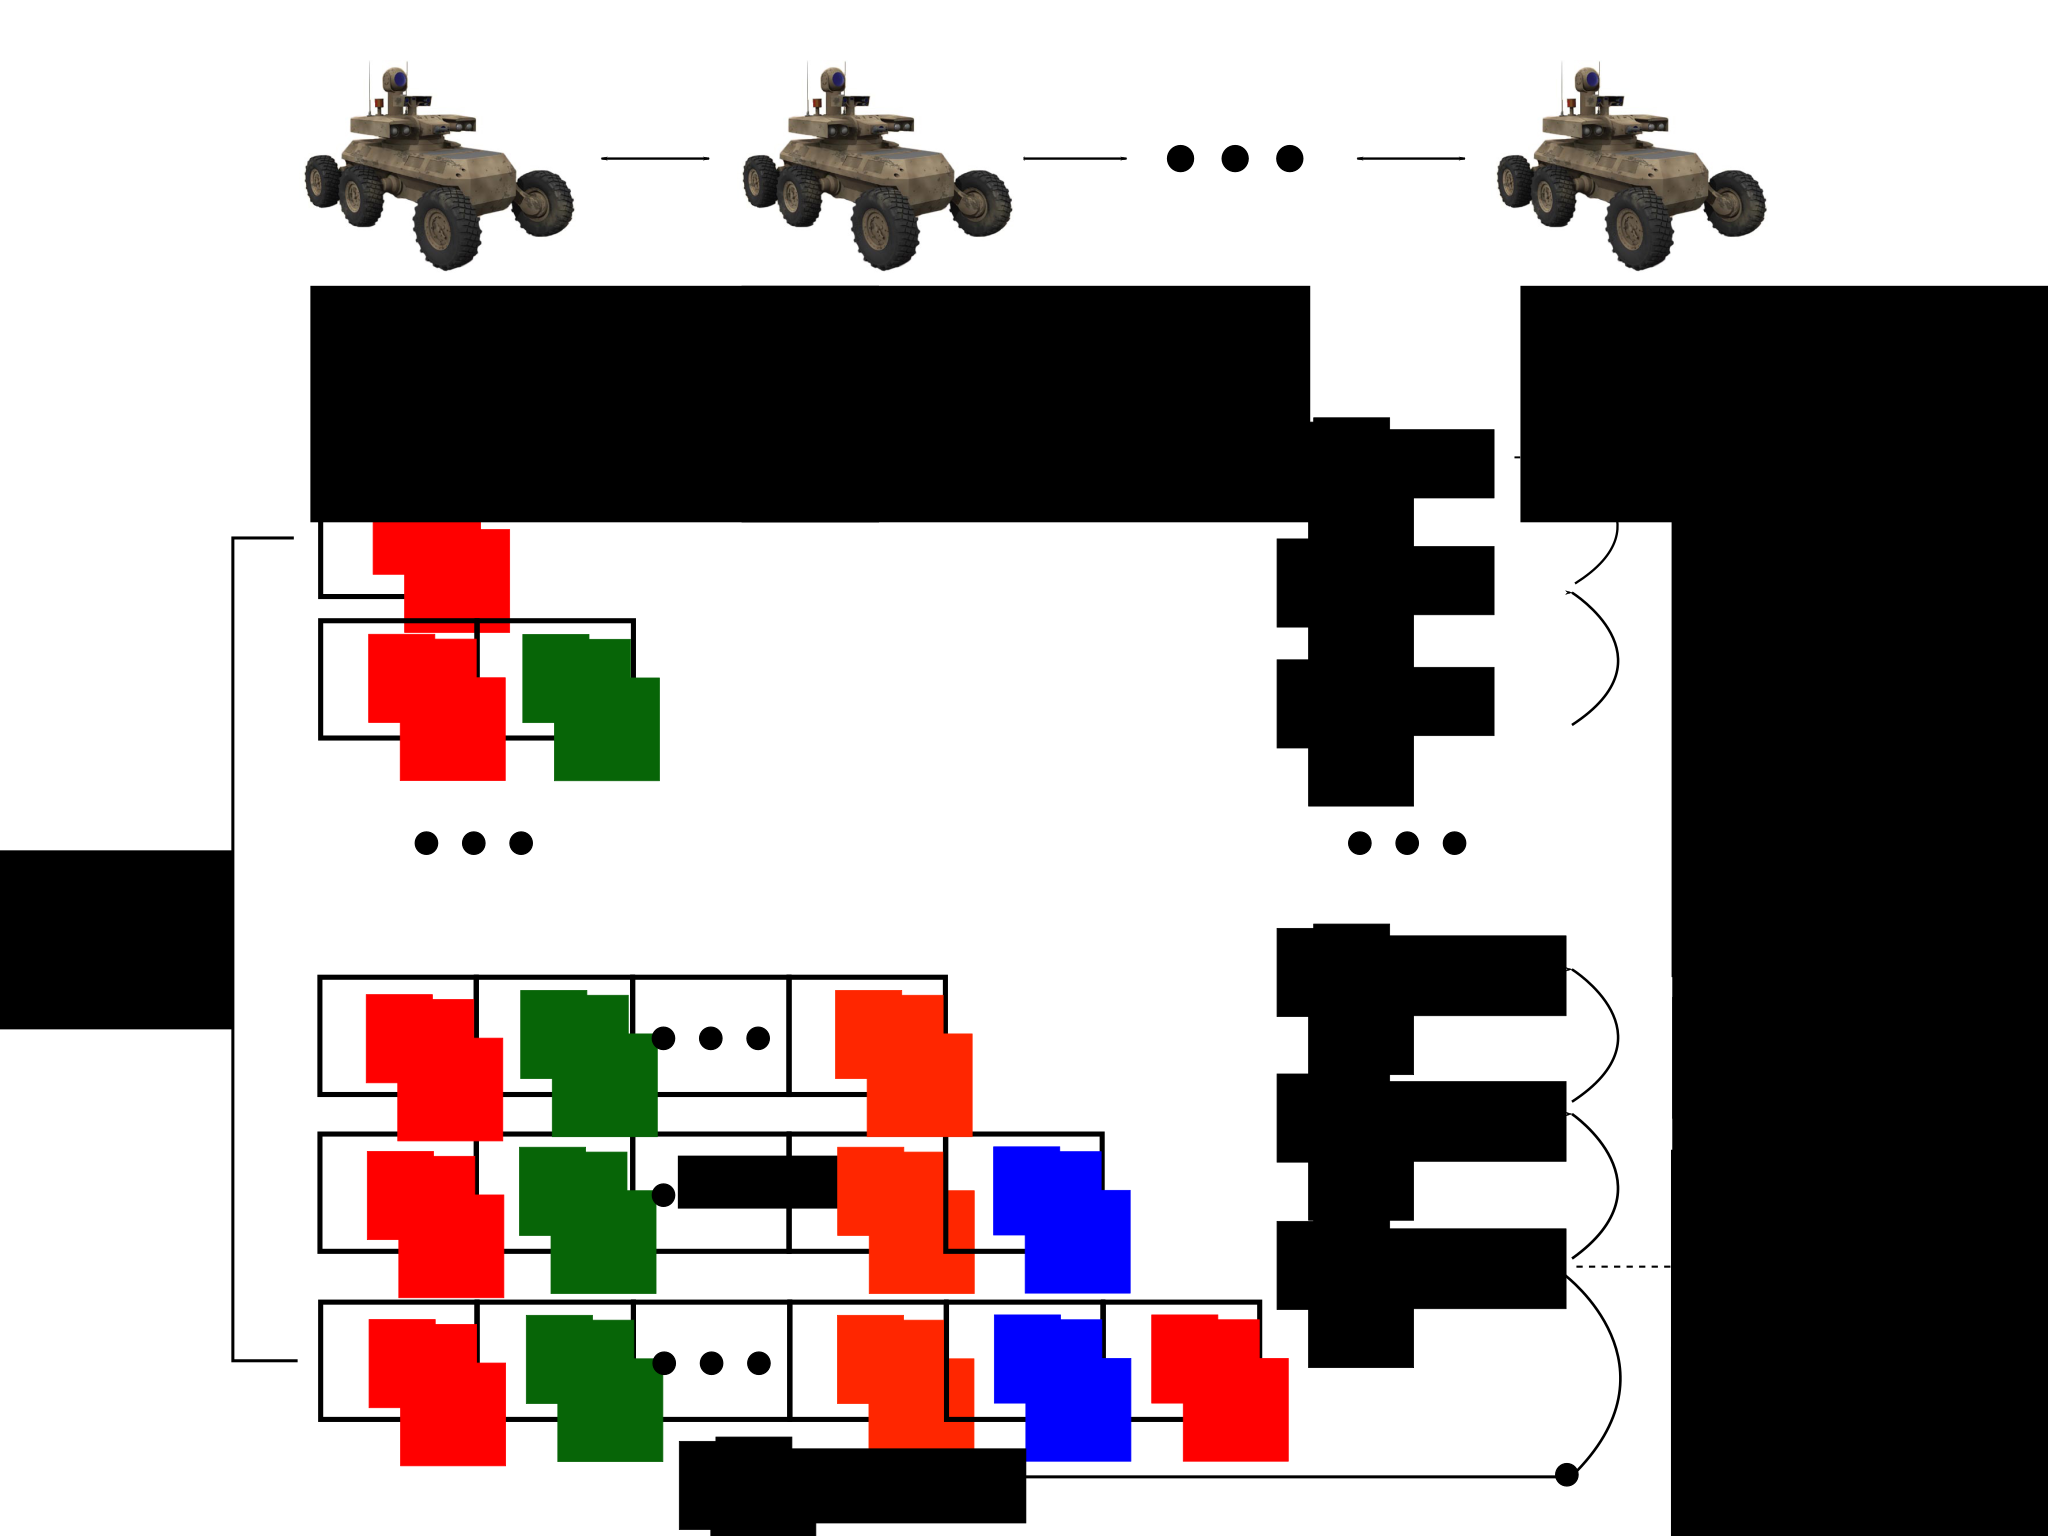
\includegraphics[width=0.51\textwidth]{figures/DBF_demo}
	\caption{Example of LIFO-DBF for $1^\text{st}$ UGV at time $k$. 	 
		Networked UGVs take a line topology. %, shown in the top. 
		The stored individual PDF is represented by $ P^1_{pdf}(k-N)$.
		The UGV first calculates $ P^1_{virt}(k-N+1)$, defined in \Cref{alg:lifo-dbf}, and then stores it as $ P^1_{pdf}(k-N+1)$. 
		Repeating DBF until obtaining $ P^1_{pdf}(k)$.
%		, which is the individual PDF at time $k$.
		In this example, $\Omega^1_{\xi}=\left\lbrace 1,2,\dots,N+1-\xi\right\rbrace $, $\xi=1,\dots,N$.}
	\label{fig:LIFO-DBF}
	\vspace{-1em}
\end{figure}

%\medskip
%\begin{rem}
	It is worth noting that, for the static target, each UGV only needs current-step CB to update individual PDFs. 
	Therefore, besides storing its own individual PDF of size $O(M^2)$, only current-step CB of size $O(N)$ is stored in an UGV's memory and all previous CBs can be discarded, which means that the size of needed memory is $O(N+M^2)$. 
	On the contrary, for the moving target, each UGV needs to store a set of historical measurements 
%	(except current step CB) triangular matrix
	of size $O(N^2)$ and an individual PDF of size $O(M^2)$. Therefore the size of the needed memory for each UGV is $O(M^2+N^2)$.
	This is generally larger than that of statistics dissemination-based methods, the memory of which is $O(M^2)$. 
	Besides, additional computation power is needed for LIFO-DBF compared to statistics dissemination-based methods.
	Therefore, LIFO-DBF sacrifices storage space and computation resource for reducing communication burden. 
	This is actually desirable for real applications as local memory of vehicles is usually abundant compared to the limited bandwidth for communication.
%\end{rem}

%\begin{algorithm}
%	\caption{LIFO-DBF Algorithm for Moving Target}\label{alg:lifo-dbf}
%	\begin{algorithmic}
%		\State For $i^\text{th}$ UGV at $k^\text{th}$ step:
%		\State After updating CB by \cref{alg:lifo},	
%		\State \textbf{(1)} The stored individual PDF is for time $(k-N)$:
%		\small\begin{equation*}
%			P^i_{stored} = P^i_{pdf}(\X_{k-N}|z^1_{1:k-N},\dots,z^N_{1:k-N}).
%		\end{equation*}\normalsize		
%		\State\textbf{(2)} Initialize a \textit{virtual PDF} by assigning the stored individual PDF to it:
%		\small\begin{equation*}
%			P^i_{virt}(\X_{k-N})= P^i_{stored}.
%%			P^i_{pdf}(\X_{k-N}|z^1_{1:k-N},\dots,z^N_{1:k-N}).
%		\end{equation*}\normalsize		
%		\State\textbf{(3)} For $\xi=1$ to $N$, iteratively repeat two steps of Bayesian filtering:
%		%	\begin{enumerate}
%		%		\item 
%		
%		\State(3.1) Prediction 
%		\small\begin{align*}
%			&P_{virt}^{pre}(\X_{k-N+\xi})\\=&\int_{S} P(\X_{k-N+\xi}|\X_{k-N+\xi-1})P^i_{virt}(\X_{k-N+\xi-1})d\X_{k-N+\xi-1}.
%		\end{align*} \normalsize
%		
%		%		\item 
%		\State(3.2) Updating
%		\small\begin{gather*}
%			P^i_{virt}(\X_{k-N+\xi})=K_\xi P_{virt}^{pre}(\X_{k-N+\xi})\prod\limits_{j\in\Omega^i_{\xi}}P(z^j_{k-N+\xi}|\X_{k-N+\xi}).\\
%			K_\xi=\left[\int_S P_{virt}^{pre}(\X_{k-N+\xi})\prod\limits_{j\in\Omega^i_{\xi}}P(z^j_{k-N+\xi}|\X_{k-N+\xi})d\X_{k-N+\xi}\right]^{-1}.
%		\end{gather*} \normalsize
%		%	\end{enumerate}
%		
%		\State(3.3) When $\xi=1$, if $z^j_{k-N+1}\neq\emptyset$ for $\forall j\in \left\lbrace1,\dots,N\right\rbrace$, then store the virtual PDF as the individual PDF for time $(k-N+1)$ to replace the old PDF:
%		\begin{equation*}
%			P^i_{pdf}(\X_{k-N+1}|z^1_{1:k-N+1},\dots,z^N_{1:k-N+1})=P^i_{virt}(\X_{k-N+1}).
%		\end{equation*}
%		
%		\State\textbf{(4)} Individual PDF of $i^\text{th}$ UGV at time $k$ is
%		$P^i_{pdf}(\X_{k}|\mathbf{z}^{i}_{1:k})=P^i_{virt}(\X_k)$.		
%	\end{algorithmic}
%\end{algorithm}

\begin{algorithm}
	\caption{LIFO-DBF Algorithm for Moving Target}\label{alg:lifo-dbf}
	\begin{algorithmic}
		\State For $i^\text{th}$ UGV at $k^\text{th}$ step:
		\State After updating CB by \cref{alg:lifo},	
%		\State \textbf{(1)} 	
		\State\textbf{(1)} Initialize a \textit{virtual PDF} by assigning the stored individual PDF to it:
		\small\begin{equation*}
		P^i_{virt}(\X_{k-N})= P^i_{stored},
		%			P^i_{pdf}(\X_{k-N}|z^1_{1:k-N},\dots,z^N_{1:k-N}).
		\end{equation*}\normalsize		
		where the stored individual PDF is for time $(k-N)$:
		\small\begin{equation*}
		P^i_{stored} = P^i_{pdf}(\X_{k-N}|z^1_{1:k-N},\dots,z^N_{1:k-N}).
		\end{equation*}\normalsize	
		\State\textbf{(2)} For $\xi=1$ to $N$, iteratively repeat two steps of Bayesian filtering:
		%	\begin{enumerate}
		%		\item 
		
		\State(2.1) Prediction 
		\small\begin{align*}
		&P_{virt}^{pre}(\X_{k-N+\xi})\\=&\int_{S} P(\X_{k-N+\xi}|\X_{k-N+\xi-1})P^i_{virt}(\X_{k-N+\xi-1})d\X_{k-N+\xi-1}.
		\end{align*} \normalsize
		
		%		\item 
		\State(2.2) Updating
		\small\begin{gather*}
		P^i_{virt}(\X_{k-N+\xi})=K_\xi P_{virt}^{pre}(\X_{k-N+\xi})\prod\limits_{j\in\Omega^i_{\xi}}P(z^j_{k-N+\xi}|\X_{k-N+\xi}).\\
		K_\xi=\left[\int_S P_{virt}^{pre}(\X_{k-N+\xi})\prod\limits_{j\in\Omega^i_{\xi}}P(z^j_{k-N+\xi}|\X_{k-N+\xi})d\X_{k-N+\xi}\right]^{-1}.
		\end{gather*} \normalsize
		%	\end{enumerate}
		
		\State(2.3) When $\xi=1$, if $z^j_{k-N+1}\neq\emptyset$ for $\forall j\in \left\lbrace1,\dots,N\right\rbrace$, then the virtual PDF is equivalent to the individual PDF for time $(k-N+1)$. Store it to replace the old PDF:
		\small\begin{equation*}
		P^i_{stored}=P^i_{virt}(\X_{k-N+1}),
%		P^i_{pdf}(\X_{k-N+1}|z^1_{1:k-N+1},\dots,z^N_{1:k-N+1})=P^i_{virt}(\X_{k-N+1}).
		\end{equation*}\normalsize
		where 
		\small\begin{equation*}
		P^i_{virt}(\X_{k-N+1})=P^i_{pdf}(\X_{k-N+1}|z^1_{1:k-N+1},\dots,z^N_{1:k-N+1}).
		\end{equation*}\normalsize
		
		\State\textbf{(3)} Individual PDF of $i^\text{th}$ UGV at time $k$ is
		$P^i_{pdf}(\X_{k}|\mathbf{z}^{i}_{1:k})=P^i_{virt}(\X_k)$.		
	\end{algorithmic}
\end{algorithm}

\section{Proof of Consistency}\label{sec:consist_proof} %and Consensus
This section proves the consistency of the maximum a posteriori (MAP) estimator of LIFO-DBF under unbiased sensors (sensors without offset).
An estimator of a state is said to be consistent if it converges in probability to the true value of the state \cite{amemiya1985advanced}.
Consistency is an important metric for stochastic filtering approaches \cite{chen2003bayesian} and it differs from the concept of consensus; consensus implies that the estimation results of all sensors converge to a same value, while consistency not only implies achieving consensus asymptotically, but also requires the estimated value converge to the true value. % (true target position).
%Therefore, consistency is a stronger concept than consensus.

We first prove the consistency for static UGVs and static target.
The consistency for  moving target and for moving UGVs are subsequently proved.
For simplicity and clarity, we assume $S$ is a finite set (e.g. a finely discretized field). %and $\xg$ is the true position of target.

%Only proofs for localizing a static target are presented, including static UGVs and moving UGVs.
%The proof of LIFO-DBF for localizing a moving target is similar but requires extra algebraic manipulation, which is omitted due to space limit.

%Considering $S$ is finite and $\xg$ is the true location of target, define an \textit{equivalent-location} set $x_{eq}\subseteq S$ such that 
%\small\begin{equation*}
%x_{eq}=\left\lbrace x\in S\arrowvert P(z_k|x^{T})=P(z_k|\xg),\; \forall z_k\in \left\lbrace 0,1\right\rbrace\right\rbrace ,
%\end{equation*}\normalsize
%i.e., $x\in x_{eq}$ gives the same measurement likelihood as $\xg$ for given UGV positions.
%%for any two parameters in $x_{eq}$, the sensor model with one of these two parameters generates equivalent probability value for the same measurement $z_k$
%Since $S$ is finite, $x_{eq}$ is also finite. 
%%Let $x_{eq,1},\dots,x_{eq,u}$ denote all equi-parameter sets that partition $X^g$ such that following properties hold:
%%\begin{enumerate}
%%	\item $\bigcup^u_{i=1} x_{eq,i}= X^g$
%%	\item $x_{eq,i}\cap x_{eq,j}=\emptyset,\;i,j\in \left\lbrace 1,\dots,u\right\rbrace ,i\neq j.$
%%\end{enumerate}
%%Without loss of generality, assume $\xg\in x_{eq,1}$, where $\xg$ denotes the actual position of the target. 
%
%%\todohere{double check if the following examples for equi-parameter set are accurate}
%
%%\begin{rem}
%%	the equivalent-location set depends on the property of the sensor. 
%%	For example, for a laser scanner with high-fidelity sensing capability, each equivalent-location set contains only a small number of target positions.
%	The reason to introduce equivalent-location set is that ghost target might exist in some special UGV arrangement and sensor types.
%	For example, for undirected binary sensors that are linearly arranged, a ghost target can exist at the mirror position of the true target.
%	When sensors are overlapped at a single point, ghost targets can exist on a circle that contains the true target.
%	In theory, DBF cannot rule out ghost targets in such cases and prior knowledge is needed for further clarification.
%%	Therefore, this study only proves the convergence to the equivalent-location set rather to the true location.
%	However, by using high-fidelity sensors, such as cameras and laser scanners, and multiple measurements from different UGV placements, equi-location set can be reduced to only contain true location of target.
	
%\end{rem}

\subsection{Static UGVs and Static Target}
%Assume $S$ is finite (e.g. a finely discretized field) and $\xg$ is the true position of target, 
The consistency of LIFO-DBF for static UGVs and target is stated as follows: 
%\todohere{converge to a set or treat the PDF as a r.v.?}
\begin{thm}\label{thm:LIFO-dbf-sta-tar}
	Assume both UGVs and the target are static, and the sensors are unbiased, then the MAP estimator of target position converges in probability to the true position of the target using LIFO-DBF, i.e.,
%	\small\begin{equation*}
%	\lim\limits_{k\rightarrow \infty}
%	P_{pdf}^i(x=\xg|\mathbf{z}^{i}_{1:k})=
%	1,\;i=1,\dots,N.
%	\end{equation*}\normalsize
	\small\begin{equation*}
	\lim\limits_{k\rightarrow \infty}
	P(\X^{MAP}=\xg|\mathbf{z}^{i}_{1:k})=
	1,\;i=1,\dots,N,
	\end{equation*}\normalsize
	where 
	\small\begin{equation*}
	\X^{MAP}=\arg\max\limits_{\X}P^i_{pdf}(\X|\mathbf{z}^{i}_{1:k}).
	\end{equation*}
\end{thm}

\begin{proof}
First we look at the asymptotic behavior of $P^i_{pdf}(\X|\mathbf{z}^{i}_{1:k})$.
The batch form of DBF at $k^\text{th}$ step is:
\small\begin{subequations}\label{eqn:bayes_batch}
	\begin{align}
		P^i_{pdf}(\X|\mathbf{z}^{i}_{1:k})&=P^i_{pdf}(\X|z^1_{1:k^i_1},\dots,z^N_{1:k^i_N})\\
		&=\frac{P^i_{pdf}(\X)\prod\limits_{j=1}^{N}\prod\limits_{l=1}^{k^i_j}P(z^j_l|\X)}{\sum\limits_{\X\in S}P^i_{pdf}(\X)\prod\limits_{j=1}^{N}\prod\limits_{l=1}^{k^i_j}P(z^j_l|\X)}\label{eqn:bayes_batch2}.
	\end{align}
\end{subequations}\normalsize
%where $P^i_{pdf}$ is $i^\text{th}$ initial individual PDF. 
The decomposition into multiplication in \Cref{eqn:bayes_batch2} results from the conditional independence of measurements given $\X$.
%It is known from \Cref{cor1} and \Cref{cor2} that $k-N<k^i_j\leq k$.\\
%\addtocounter{equation}{-1}\\


Comparing the conditional probability of an arbitrary position $x\in S$ with that of target position $\xg$:
%$P^i_{pdf}(\X=x|\mathbf{z}^{i}_{1:k})$ with $P^i_{pdf}(\X=\xg|\mathbf{z}^{i}_{1:k})$ yields
\small\begin{equation}\label{eqn:cmp}
\frac{P^i_{pdf}(\X=x|\mathbf{z}^{i}_{1:k})}{P^i_{pdf}(\X=\xg|\mathbf{z}^{i}_{1:k})}=\frac{P^i_{pdf}(x)\prod\limits_{j=1}^{N}\prod\limits_{l=1}^{k^i_j}P(z^j_l|x)}{P^i_{pdf}(\xg)\prod\limits_{j=1}^{N}\prod\limits_{l=1}^{k^i_j}P(z^j_l|\xg)}.\footnote{For the purpose of simplicity, we abbreviate $P^i_{pdf}(\X=x)$ and $P(z^j_l|\X=x)$ as $P^i_{pdf}(x)$ and $P(z^j_l|x)$ in this proof.}
\end{equation}\normalsize

Take the logarithm of \Cref{eqn:cmp} and average it over $k$ steps:
\small\begin{equation}\label{eqn:cmp_log}
 \frac{1}{k}\ln\frac{P^i_{pdf}(\X=x|\mathbf{z}^{i}_{1:k})}{P^i_{pdf}(\X=\xg|\mathbf{z}^{i}_{1:k})}=\frac{1}{k}\ln\frac{P^i_{pdf}(x)}{P^i_{pdf}(\xg)}+\sum\limits_{j=1}^{N}\frac{1}{k}\sum\limits_{l=1}^{k^i_j}\ln\frac{P(z^j_l|x)}{P(z^j_l|\xg)}.
\end{equation}\normalsize

Since $P^i_{pdf}(x)$ and $P^i_{pdf}(\xg)$ are bounded and $P^i_{pdf}(\X)$ is initialized such that $P^i_{pdf}(\xg)\neq 0$, then
\small\begin{equation*}\label{eqn:cmp_lim1}
\lim\limits_{k\rightarrow \infty}\frac{1}{k}\ln\frac{P^i_{pdf}(x)}{P^i_{pdf}(\xg)}= 0.
\end{equation*}\normalsize

Utilizing the facts: (1) $z^j_l$ are conditionally independent samples from $P(z^j_l|\xg)$ and (2) $k-N<k^i_j\leq k$, the law of large numbers yields
%\small\begin{equation*}
%\frac{1}{k}\sum\limits_{l=1}^{k^i_j}z^j_l\overset{P}{\longrightarrow}p^{j^*}_{1},\quad 
%\frac{1}{k}(k^i_j-\sum\limits_{l=1}^{k^i_j}z^j_l)\overset{P}{\longrightarrow}1-p^{j^*}_{1},
%\end{equation*}\normalsize
%Then, 
\small\begin{subequations}\label{eqn:cmp_lim2}
\begin{align} 
\frac{1}{k}\sum\limits_{l=1}^{k^i_j}\ln\frac{P(z^j_l|x)}{P(z^j_l|\xg)}&\overset{P}{\longrightarrow}\mathbb{E}_{z^j_l} \left[\ln\frac{P(z^j_l|x)}{P(z^j_l|\xg)}\right]\\
&=\int_{z^j_l} P(z^j_l|\xg)\ln\frac{P(z^j_l|x)}{P(z^j_l|\xg)} dz^j_l\\
&=-D_{KL}\left(P(z^j_l|\xg)\|P(z^j_l|x)\right),
\end{align}
\end{subequations}\normalsize
where ``$\overset{P}{\longrightarrow}$" represents ``convergence in probability'' and $D_{KL}(P_1\|P_2)$ denotes the Kullback-Leibler (KL) divergence between two probability distributions $P_1$ and $P_2$.
The KL divergence has the property \cite{mackay2003information} that $\forall P_1,\,P_2$,
\begin{equation*}
D_{KL}(P_1\|P_2)\leq 0, \text{ equality holds iff } \; P_1=P_2.
\end{equation*}
%\begin{subequations}
%	\begin{gather*}
%	 D_{KL}(P_1\|P_2)\leq 0,\\
%	\text{equality holds iff } \; P_1=P_2.
%	\end{gather*}
%\end{subequations}
This leads to the following results:
%\begin{subequations}
%	\begin{align}
%		\frac{1}{k}\sum\limits_{l=1}^{k^i_j}\ln\frac{P(z^j_l|x)}{P(z^j_l|\xg)}<0,&\quad x\neq \xg\\
%		\frac{1}{k}\sum\limits_{l=1}^{k^i_j}\ln\frac{P(z^j_l|x)}{P(z^j_l|\xg)}=0,&\quad x= \xg.
%	\end{align}
%\end{subequations}

\begin{equation*}
	\lim\limits_{k\rightarrow \infty}\frac{1}{k}\sum\limits_{l=1}^{k^i_j}\ln\frac{P(z^j_l|x)}{P(z^j_l|\xg)}\;
	\begin{cases}
		<0,&\quad \text{if}\; x\neq \xg\\
		=0,&\quad \text{if}\; x= \xg
	\end{cases}.
\end{equation*}

Then by considering the limit of \Cref{eqn:cmp_log} when $k\rightarrow\infty$, we get:
%\begin{subequations}
%	\begin{align}
%	\lim\limits_{k\rightarrow \infty}\frac{1}{k}\ln\frac{P^i_{pdf}(x|\mathbf{z}^{i}_{1:k})}{P^i_{pdf}(\xg|\mathbf{z}^{i}_{1:k})}<0,&\quad x\neq \xg\label{subeqn:limit1}\\
%	\lim\limits_{k\rightarrow \infty}\frac{1}{k}\ln\frac{P^i_{pdf}(x|\mathbf{z}^{i}_{1:k})}{P^i_{pdf}(\xg|\mathbf{z}^{i}_{1:k})}=0,&\quad x= \xg\label{subeqn:limit2}.
%	\end{align}
%\end{subequations}

\begin{equation}\label{subeqn:limit}
	\lim\limits_{k\rightarrow \infty}\frac{1}{k}\ln\frac{P^i_{pdf}(x|\mathbf{z}^{i}_{1:k})}{P^i_{pdf}(\xg|\mathbf{z}^{i}_{1:k})}\;
	\begin{cases}
		<0,&\quad \text{if}\; x\neq \xg\\
		=0,&\quad \text{if}\; x= \xg
	\end{cases}.
\end{equation}

\Cref{subeqn:limit} implies that
%\begin{subequations}
%	\begin{align}
%	\frac{P^i_{pdf}(x|\mathbf{z}^{i}_{1:k})}{P^i_{pdf}(\xg|\mathbf{z}^{i}_{1:k})}\overset{P}{\longrightarrow}0,&\quad x\neq \xg\\
%	\frac{P^i_{pdf}(x|\mathbf{z}^{i}_{1:k})}{P^i_{pdf}(\xg|\mathbf{z}^{i}_{1:k})}\overset{P}{\longrightarrow}1,&\quad x= \xg.
%	\end{align}
%\end{subequations}

\begin{equation*}
	\frac{P^i_{pdf}(x|\mathbf{z}^{i}_{1:k})}{P^i_{pdf}(\xg|\mathbf{z}^{i}_{1:k})}\overset{P}{\longrightarrow}
	\begin{cases}
		0,&\quad \text{if}\; x\neq \xg\\
		1,&\quad \text{if}\; x= \xg
	\end{cases}.
\end{equation*}

Therefore,
\small\begin{equation*}
\lim\limits_{k\rightarrow \infty}
P_{pdf}^i(\X=\xg|\mathbf{z}^{i}_{1:k})=1.
\end{equation*}\normalsize
Thus
\small\begin{equation*}
\lim\limits_{k\rightarrow \infty}
P(\X^{MAP}=\xg|\mathbf{z}^{i}_{1:k})=1.
\end{equation*}\normalsize

%Note that the right-hand side of \Cref{eqn:cmp_lim2} achieves maximum value 0 if and only if $p^{j}_{1}=p^{j^*}_{1}$. 
%Define 
%\small\begin{equation*}
%c(x)=\sum\limits_{j=1}^{N}p^{j^*}_{1}\ln \frac{p^{j}_{1}}{p^{j^*}_{1}}+(1-p^{j^*}_{1})\ln\frac{1-p^{j}_{1}}{1-p^{j^*}_{1}}.
%\end{equation*}\normalsize
%
%Considering \Cref{eqn:cmp_lim1} and \Cref{eqn:cmp_lim2}, the limit of \Cref{eqn:cmp_log} is
%\small \begin{equation}\label{eqn:lim}
%% \lim\limits_{k\rightarrow \infty}
% \frac{1}{k}\ln\frac{P^i_{pdf}(x|\mathbf{z}^{i}_{1:k})}{P^i_{pdf}(\xg|\mathbf{z}^{i}_{1:k})}\overset{P}{\longrightarrow}c(x)
%% \sum\limits_{j=1}^{N}p^*_j\ln \frac{p_j}{p^*_j}+(1-p^*_j)\ln \frac{1-p_j}{1-p^*_j}
%\end{equation}\normalsize
% 
%It follows from \Cref{eqn:lim} that
%\small\begin{equation}\label{eqn:lim2}
%\frac{P^i_{pdf}(x|\mathbf{z}^{i}_{1:k})}{P^i_{pdf}(\xg|\mathbf{z}^{i}_{1:k})e^{c(x)k}}\overset{P}{\longrightarrow}1.
%\end{equation}\normalsize
%
%Define the set $\bar{X}^T=S\setminus \left\lbrace \xg\right\rbrace$ and $c_M=\max\limits_{x\in\bar{X}^T}c(x)$.
%Then $c_M<0$.
%Summing \Cref{eqn:lim2} over $\bar{X}^T$ yields
%\small\begin{equation}\label{eqn:lim3}
%\frac{\sum\limits_{x\in \bar{X}^T}P^i_{pdf}(x|\mathbf{z}^{i}_{1:k})e^{\left[c_M-c(x)\right]k}}{{P^i_{pdf}(\xg|\mathbf{z}^{i}_{1:k})}e^{c_Mk}}\overset{P}{\longrightarrow} |\bar{X}^T|,
%\end{equation}\normalsize
%where $|\bar{X}^T|$ denotes the cardinality of $\bar{X}^T$.
%
%Since $c_M<0$,  ${P^i_{pdf}(\xg|\mathbf{z}^{i}_{1:k})}e^{c_Mk}{\longrightarrow}0$, \Cref{eqn:lim3} implies
%\begin{equation}\label{eqn:lim4}
%\sum\limits_{x\in \bar{X}^T}P^i_{pdf}(x|\mathbf{z}^{i}_{1:k})e^{\left[c_M-c(x)\right]k}\overset{P}{\longrightarrow}0.
%\end{equation}
%
%Utilizing the relation 
%\begin{equation*}
%0\leq P^i_{pdf}(x|\mathbf{z}^{i}_{1:k})\leq P^i_{pdf}(x|\mathbf{z}^{i}_{1:k})e^{\left[c_M-c(x)\right]k},
%\end{equation*}
%it can be derived from \Cref{eqn:lim4} that
%\small\begin{equation*}
%\sum\limits_{x\in \bar{X}^T}P^i_{pdf}(x|\mathbf{z}^{i}_{1:k})\overset{P}{\longrightarrow} 0.
%\end{equation*}\normalsize
%Therefore,
%\small\begin{equation*}
%	\lim\limits_{k\rightarrow \infty}
%	P(x=\xg|\mathbf{z}^{i}_{1:k})=1-\lim\limits_{k\rightarrow \infty}\sum\limits_{x\in \bar{X}^T}P^i_{pdf}(x|\mathbf{z}^{i}_{1:k})=1.
%\end{equation*}\normalsize
\end{proof}

\subsection{Static UGVs and Moving Target}
The consistency of LIFO-DBF for static UGVs and moving target is stated as follows:
\begin{thm}\label{thm:LIFO-dbf-mov-tar}
	Assume UGVs are static, sensors are unbiased and the target is moving deterministically, then the MAP estimator of the target position converges in probability to the true position of the target using LIFO-DBF, i.e.,
	\small\begin{equation*}
	\lim\limits_{k\rightarrow \infty}P(\X^{MAP}_k=\xg_k|\mathbf{z}^i_{1:k})=
	1,\;i=1,\dots,N.
%	P(x_k^g=x_k^{g^*}|\mathbf{z}^i_{1:k})=1,\;i=1,\dots,N.
	\end{equation*}\normalsize
\end{thm}
\begin{proof}
	Since the target motion model is deterministic, as defined in \Cref{eqn:markov_model}, the integration in the prediction step (\Cref{eqn:bayes_pred}) can be removed, as no uncertainty exists in $P(\X_k|\X_{k-1})$.
	
	\Cref{eqn:bayes_batch} now becomes
	\small\begin{subequations}
		\begin{align*}
		P^i_{pdf}(\X_k|\mathbf{z}^{i}_{1:k})&=P^i_{pdf}(\X_k|z^1_{1:k^i_1},\dots,z^N_{1:k^i_N})\\
		&=\frac{P^i_{pdf}(\X_0)\prod\limits_{j=1}^{N}\prod\limits_{l=1}^{k^i_j}P(z^j_l|\X_l)P(\X_l|\X_{l-1})}{\sum\limits_{\X_0,\dots,\X_k\in S}P^i_{pdf}(\X_0)\prod\limits_{j=1}^{N}\prod\limits_{l=1}^{k^i_j}P(z^j_l|\X_l)P(\X_l|\X_{l-1})}.
		\end{align*}
	\end{subequations}\normalsize
	The term $P(\X_l|\X_{l-1})$ cancels when dividing $P^i_{pdf}(\X_k=x_k|\mathbf{z}^{i}_{1:k})$ by $P^i_{pdf}(\X_k=\xg_k|\mathbf{z}^{i}_{1:k})$, thus yielding the same result as \Cref{eqn:cmp}. The rest of the proof is similar to that of \Cref{thm:LIFO-dbf-sta-tar}.
\end{proof}


\begin{figure}%[thpb]
	\centering
	\begin{subfigure}[b]{0.24\textwidth}
		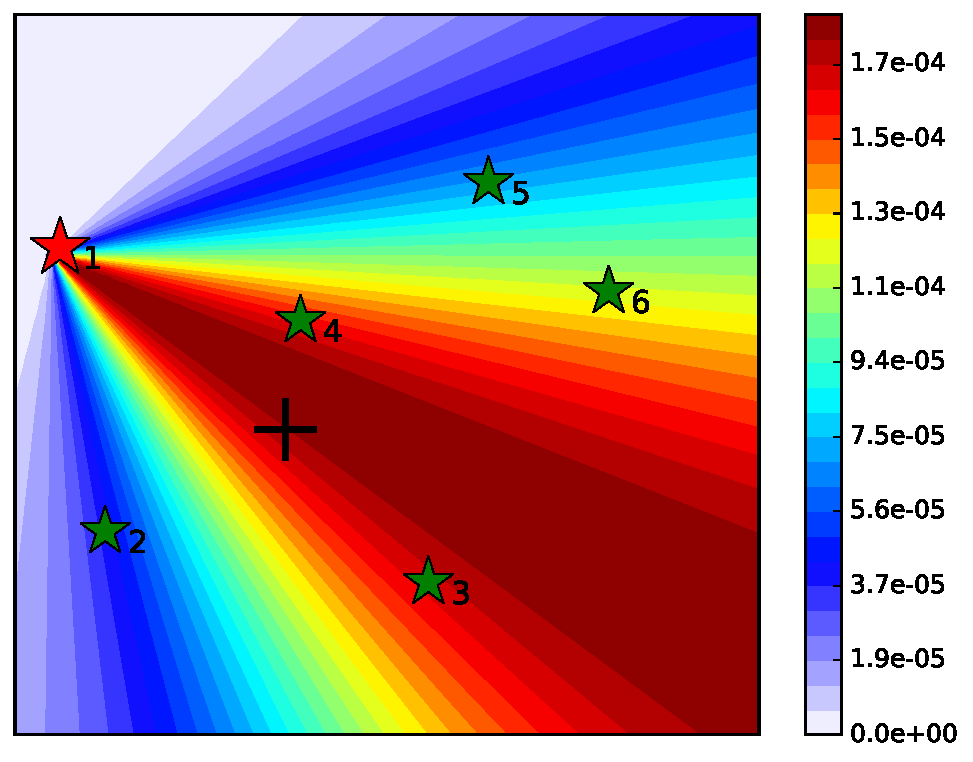
\includegraphics[width=\textwidth]{figures/brg_sta_sen_sta_tar_rbt1_step1}
		\caption{Step 1}\label{fig:sta_sen_sta_tar_sing1}
	\end{subfigure}
	\begin{subfigure}[b]{0.24\textwidth}
		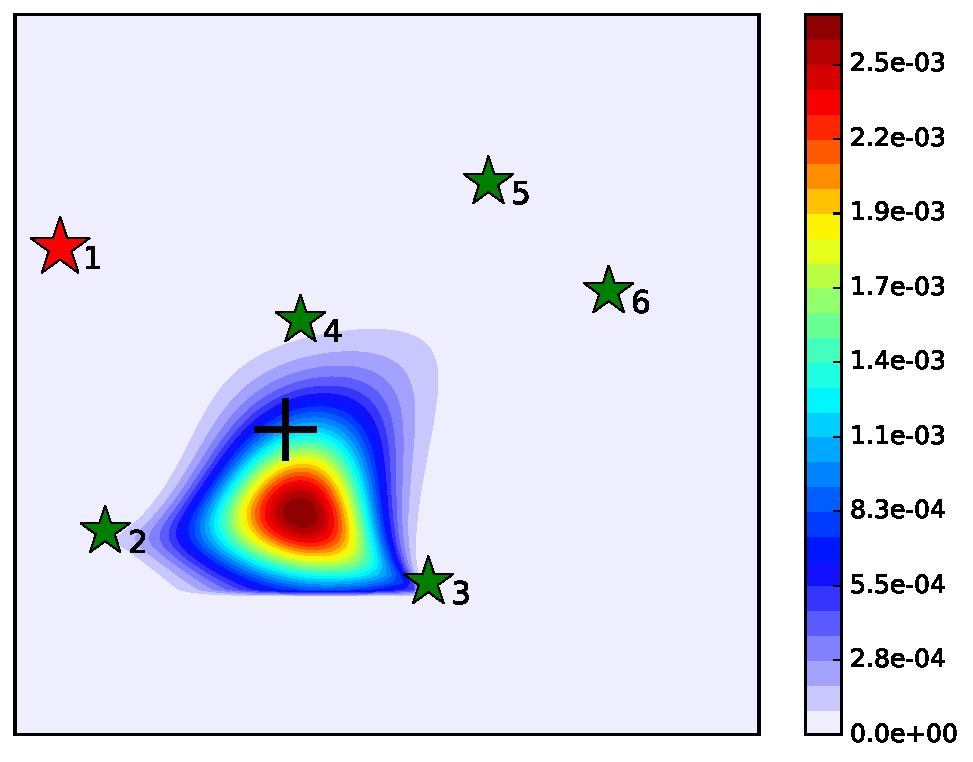
\includegraphics[width=\textwidth]{figures/brg_sta_sen_sta_tar_rbt1_step3}
		\caption{Step 3}\label{fig:sta_sen_sta_tar_sing2}
	\end{subfigure}
	\begin{subfigure}[b]{0.24\textwidth}
		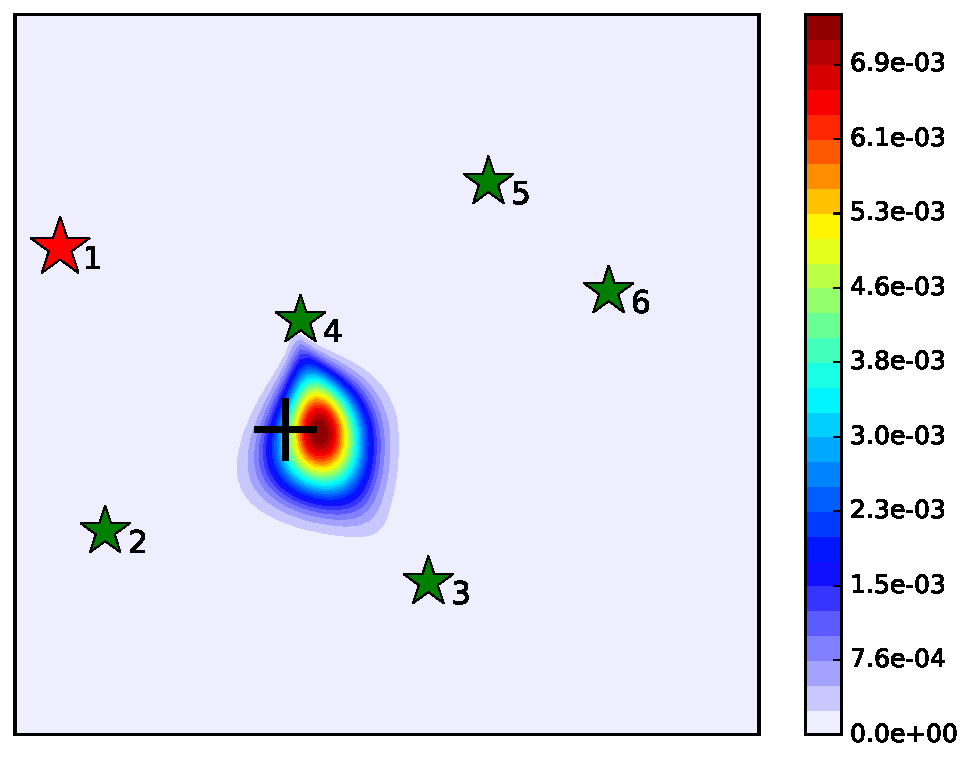
\includegraphics[width=\textwidth]{figures/brg_sta_sen_sta_tar_rbt1_step5}
		\caption{Step 5}\label{fig:sta_sen_sta_tar_sing3}
	\end{subfigure}
	\begin{subfigure}[b]{0.24\textwidth}
		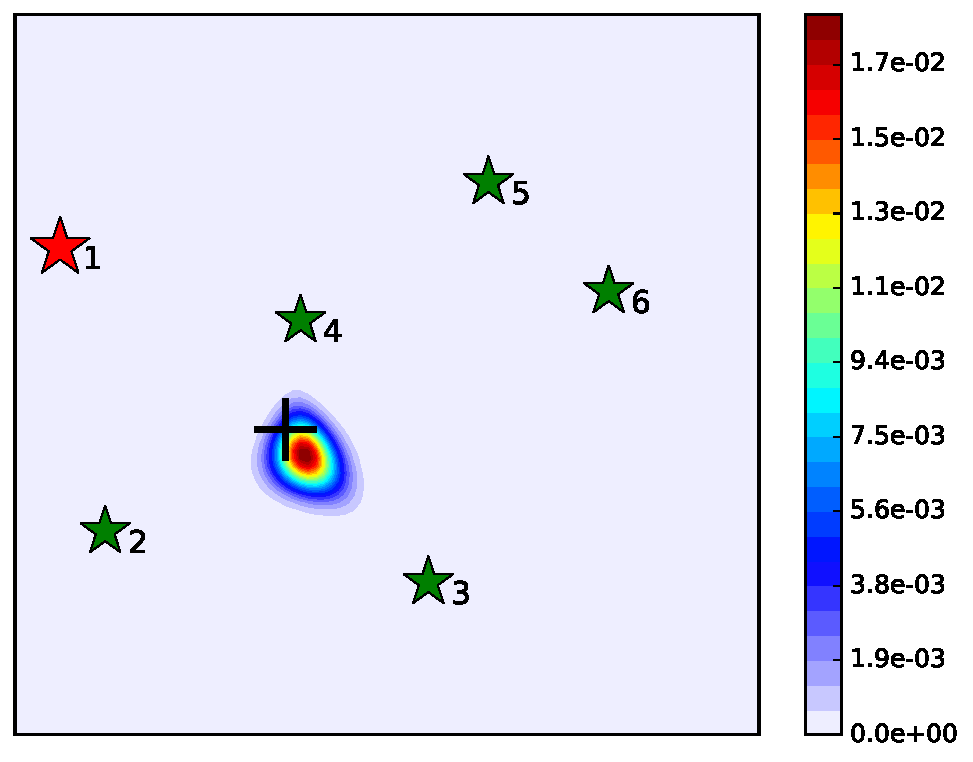
\includegraphics[width=\textwidth]{figures/brg_sta_sen_sta_tar_rbt1_step10}
		\caption{Step 10}\label{fig:sta_sen_sta_tar_sing4}
	\end{subfigure}
	\begin{subfigure}[b]{0.24\textwidth}
		%		\includegraphics[width=\textwidth]{figures/test}
		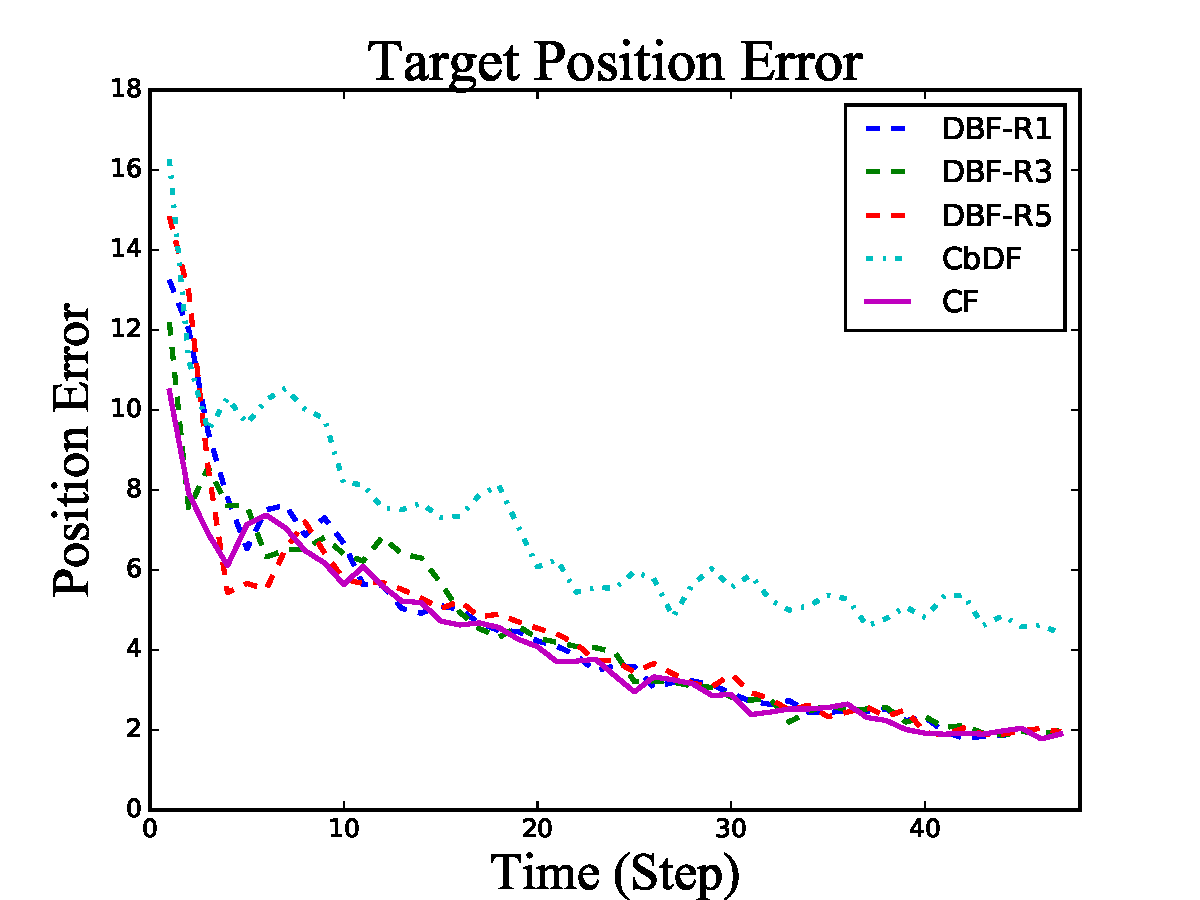
\includegraphics[width=\textwidth]{figures/brg_sta_sen_sta_tar_pos_err}
		\caption{Position Error}\label{fig:sta_sen_sta_tar_pos_err}
	\end{subfigure}
	\begin{subfigure}[b]{0.24\textwidth}
		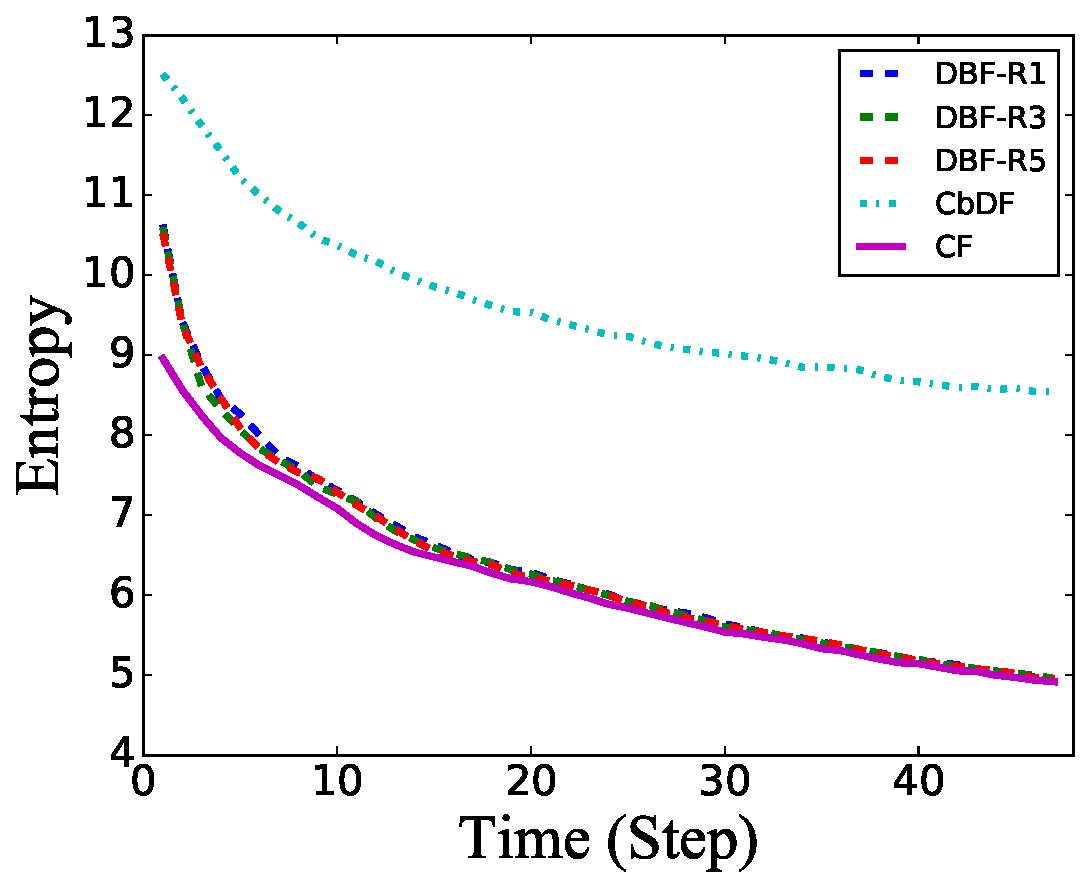
\includegraphics[width=\textwidth]		{figures/brg_sta_sen_sta_tar_entropy}%{figures/test2}
		\caption{Entropy of Individual PDF}\label{fig:sta_sen_sta_tar_entropy}
	\end{subfigure}
	\caption{(a)-(d) The $1^\text{st}$ UGV's individual PDF at different times. 
%		The red star denotes the UGV whose individual PDF is shown. 
The cross stands for the target. Note that the value of the color bar varies among different figures. (e) Average position estimation error of the $1^\text{st}$, $3^\text{rd}$ and $5^\text{th}$ UGV's LIFO-DBF, the CbDF and the CF. (f) Average entropy of individual PDFs.}
	\label{fig:sta_sen_sta_tar}
	%	\vspace{-1.2em}
\end{figure}

\begin{figure}%[thpb]
	\centering
	\begin{subfigure}[b]{0.24\textwidth}
		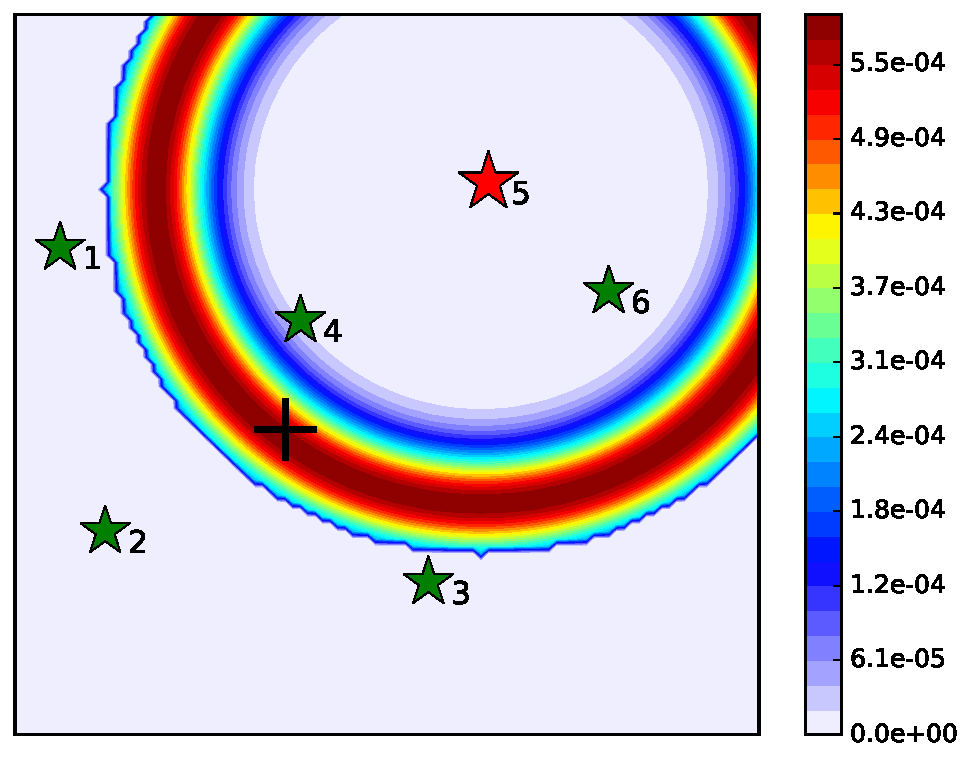
\includegraphics[width=\textwidth]{figures/hetero_sta_sen_sta_tar_rbt5_step1}
		\caption{Step 1}\label{fig:htr_sta_sen_sta_tar_sing1}
	\end{subfigure}
	\begin{subfigure}[b]{0.24\textwidth}
		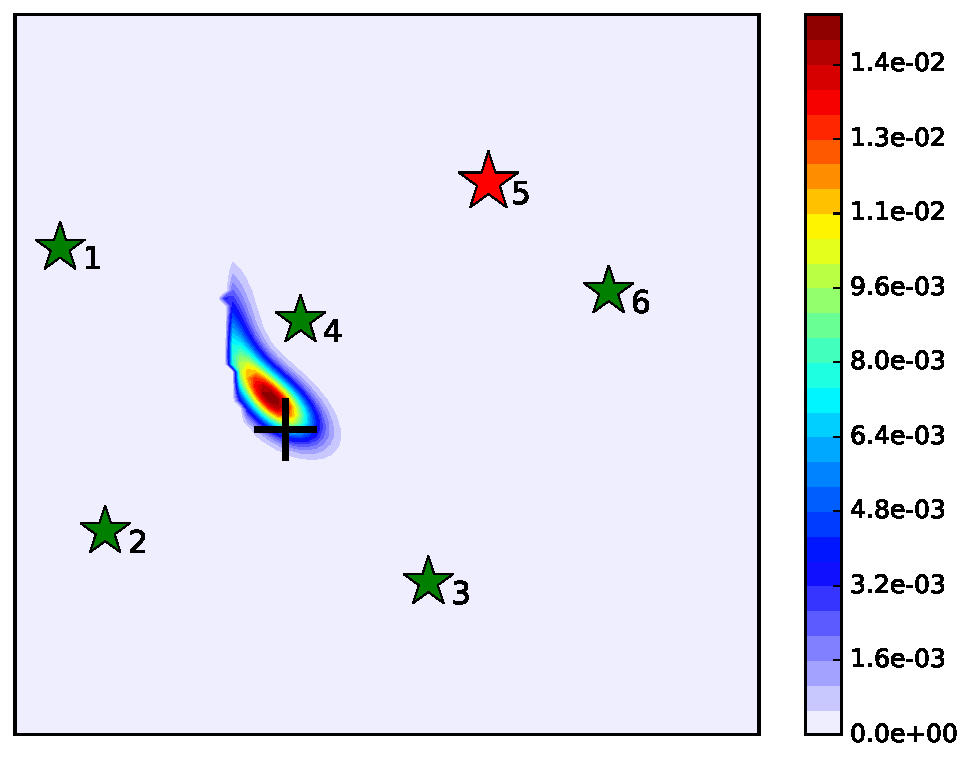
\includegraphics[width=\textwidth]{figures/hetero_sta_sen_sta_tar_rbt5_step3}
		\caption{Step 3}\label{fig:htr_sta_sen_sta_tar_sing2}
	\end{subfigure}
	\begin{subfigure}[b]{0.24\textwidth}
		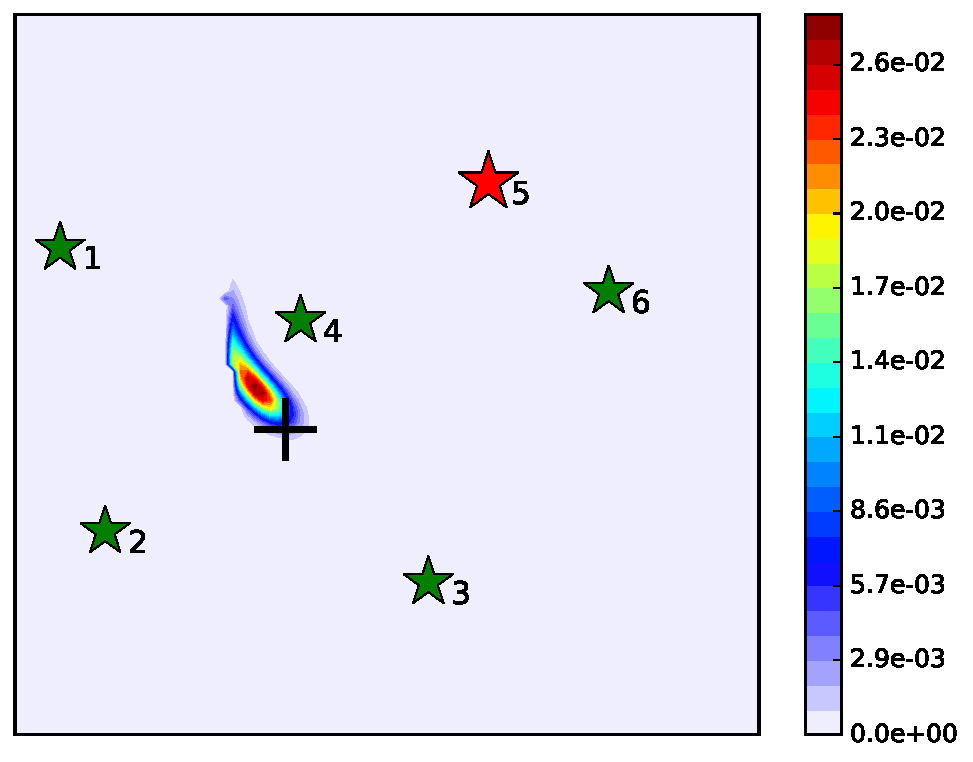
\includegraphics[width=\textwidth]{figures/hetero_sta_sen_sta_tar_rbt5_step5}
		\caption{Step 5}\label{fig:htr_sta_sen_sta_tar_sing3}
	\end{subfigure}
	\begin{subfigure}[b]{0.24\textwidth}
		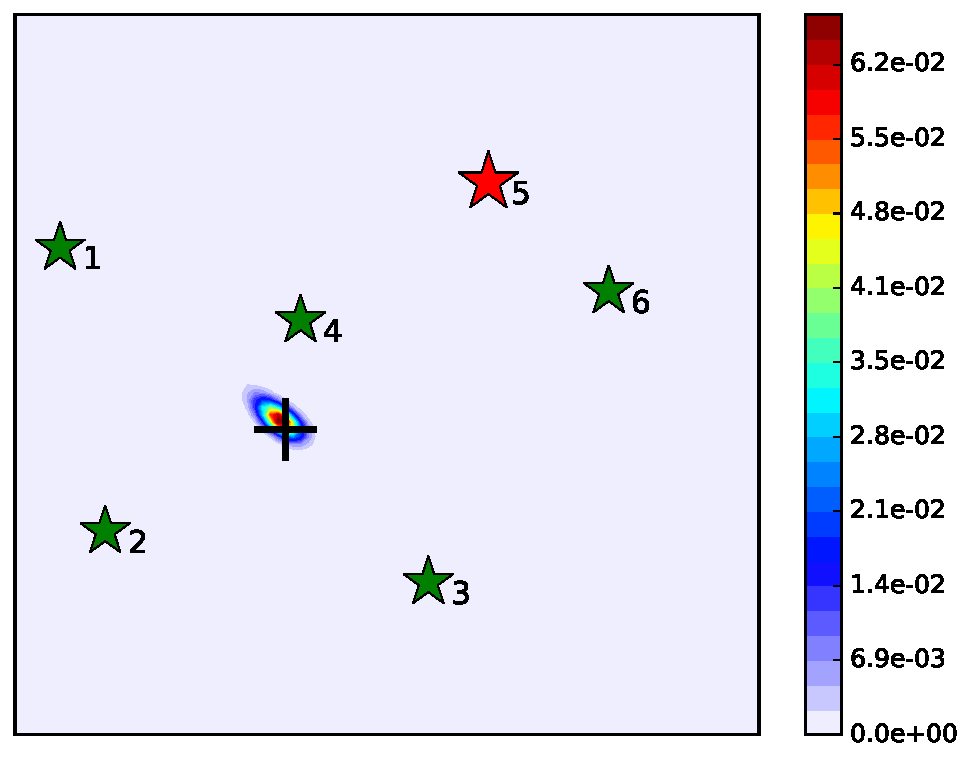
\includegraphics[width=\textwidth]{figures/hetero_sta_sen_sta_tar_rbt5_step10}
		\caption{Step 10}\label{fig:htr_sta_sen_sta_tar_sing4}
	\end{subfigure}
	\begin{subfigure}[b]{0.24\textwidth}
		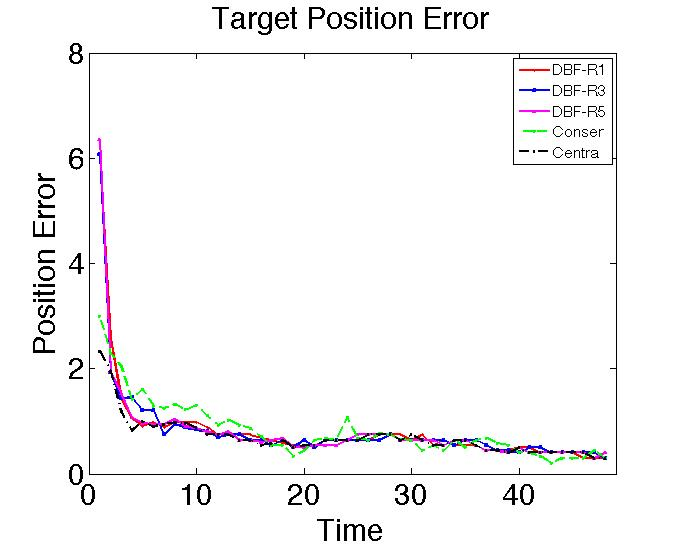
\includegraphics[width=\textwidth]{figures/hetero_sta_sen_sta_tar_pos_err}
		\caption{Position Error}\label{fig:htr_sta_sen_sta_tar_pos_err}
	\end{subfigure}
	\begin{subfigure}[b]{0.24\textwidth}
		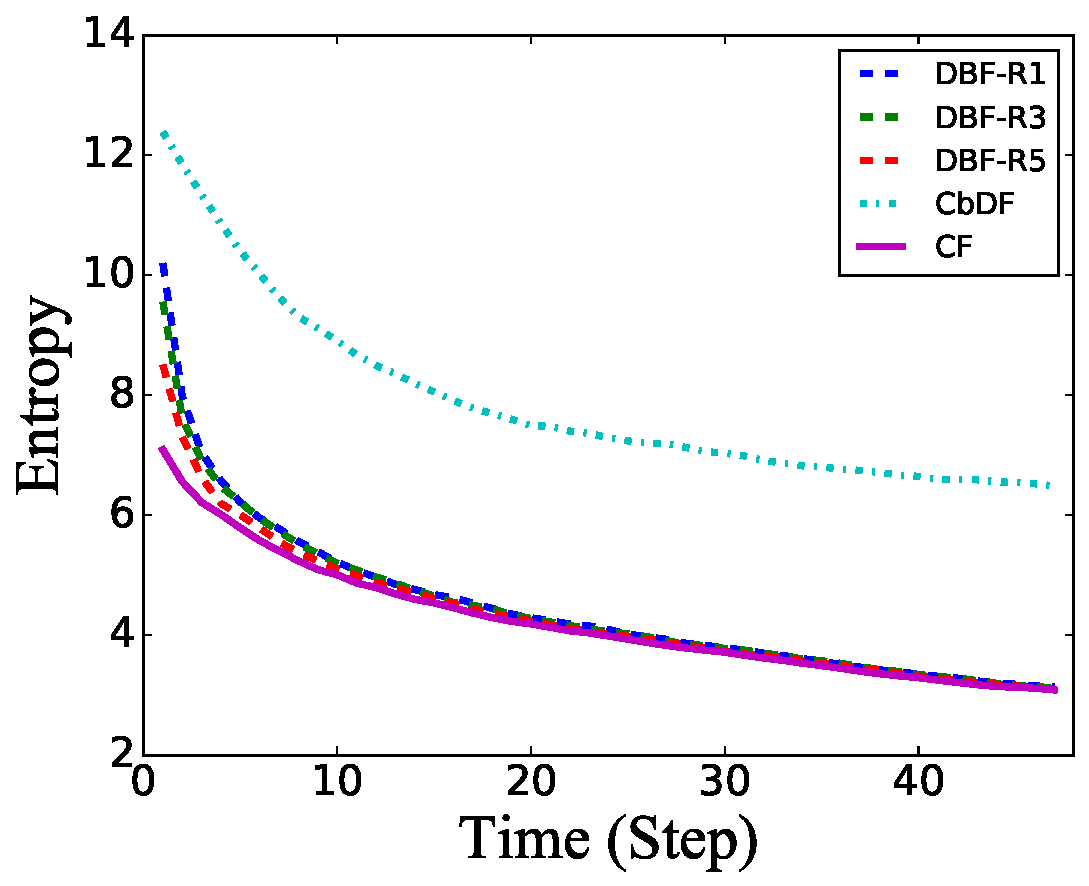
\includegraphics[width=\textwidth]{figures/hetero_sta_sen_sta_tar_entropy}
		\caption{Entropy of Individual PDF}\label{fig:htr_sta_sen_sta_tar_entropy}
	\end{subfigure}
	\caption{(a)-(d) The $5^\text{th}$ UGV's individual PDF at different times. (e) Average position estimation error. (f) Average entropy of individual PDFs.}
	\label{fig:htr_sta_sen_sta_tar}
	%	\vspace{-1.2em}
\end{figure}

\subsection{Moving UGVs}
This subsection considers the case of using moving UGVs to localize a target, either static or moving.
The difficulty of consistency proof for this case lies in the fact that each UGV makes measurements at multiple positions.
Here, the main idea of the proof is to classify UGV measurement positions into two disjoint sets: \textit{infinite-measurement spots} that contain positions where a UGV visits infinitely many times as time tends to infinity, and \textit{finite-measurement spots} that contain positions where the UGV visits finitely many times (i.e., the UGV does not visit again after a finite time period).
%, as $k\rightarrow\infty$.
Before stating the main theorem, the following lemma is introduced.
\begin{lem}\label{lem1}
	For a set of UGVs moving within a collection of finite positions, each UGV has at least one position where infinite measurements are made as $k$ tends to infinity.
\end{lem}

\begin{proof}
Let $n^{i,k}_s$ denote the times that $i^\text{th}$ UGV visits $s^\text{th}$ position up to time $k$. Then, $\sum\limits_{s\in S} n^{i,k}_s=k$. It is straightforward to see that $\exists n^{i,k}_s,$ such that $n^{i,k}_s\rightarrow \infty,$ as $k\rightarrow \infty$.
\end{proof}
\medskip

\begin{thm}\label{thm:LIFO-dbf-mov-sen}
	Assume UGVs move within a collection of finite positions and sensors are unbiased, then the MAP estimator of target position converges in probability to the true position of the target using LIFO-DBF, i.e.,
	\small\begin{equation*}
		\lim\limits_{k\rightarrow \infty}
		P(\X^{MAP}_k=\xg_k|\mathbf{z}^i_{1:k})=1,\;i=1,\dots,N.
%		P(x=\xg|\mathbf{z}^i_{1:k})=1,\;i=1,\dots,N.
	\end{equation*}\normalsize
\end{thm}

\begin{proof}
	Without loss of generality, we assume the target is static. The proof when target is moving deterministically is similar.
According to \Cref{thm:LIFO-dbf-sta-tar}, the batch form of DBF at $k^\text{th}$ step is
\small\begin{equation}\label{eqn:cmp2}
\frac{P^i_{pdf}(\X=x|\mathbf{z}^i_{1:k})}{P^i_{pdf}(\X=\xg|\mathbf{z}^i_{1:k})}=\frac{P^i_{pdf}(x)\prod\limits_{j=1}^{N}\prod\limits_{l=1}^{k^i_j}P(z^j_l|x;x^j_l)}{P^i_{pdf}(\xg)\prod\limits_{j=1}^{N}\prod\limits_{l=1}^{k^i_j}P(z^j_l|\xg;x^j_l)}.
\end{equation}\normalsize

The only difference from \Cref{eqn:cmp} is that $P(z^j_l|x;x^j_l)$ in \Cref{eqn:cmp2} varies as the UGV moves.
%, needs to be grouped according to the UGV position. 
For each UGV, there exists at least one position where infinite measurements are made as $k\rightarrow \infty$, according to \Cref{lem1}. 
%All positions can be classified into finite-measurement spots and infinite-measurement spots. 
For the finite-measurement spots, by referring to \Cref{eqn:cmp_lim2}, it is easy to know that their contribution to \Cref{eqn:cmp_log} diminishes when $k\rightarrow \infty$.
Therefore, proof using \Cref{eqn:cmp2} can be reduced to only considering infinite-measurement spots and the rest of proof is similar to that of \Cref{thm:LIFO-dbf-sta-tar}.
\end{proof}

\begin{rem}
	The assumption of unbiased sensors are important for the consistency of the estimator. In fact, with unknown non-zero bias, the distribution of $z^j_l$ differs from $P(z^j_l|\xg)$, which invalidates the derivation in \Cref{eqn:cmp_lim2} and the consistency proof. 
	This assumption also makes intuitive sense.
	In the extreme case, if each sensor has a very large unknown measurement offset, then the estimated target position of each sensor (without communicating with other sensors) will be very different from each other's.
	Therefore, no common target position can be correctly obtained when they fuse measurements.
\end{rem}
\medskip
%\begin{rem}
%%	When $x_{eq}$ only contains $x^{T^{*}}$, consistency means the estimated target position converges to true target position in probability. Additionally, 
%	Consistency implies that all individual PDFs converge to the same distribution (true target PDF), thus the consensus is also guaranteed.
%	It must be noted that traditional statistics dissemination-based methods only ensure consensus of individual PDFs \cite{bandyopadhyay2014distributed,julian2012distributed}. 
%	To the best knowledge of authors, there is no proof of consistency on estimated target position.
%%	that guarantees the agreed PDF is close to the true target PDF.
%%	 of individual PDFs.
%%	In fact, the statistics dissemination-based methods can ensure the convergence of the state estimate among UGVs. 
%%	However, there's no guarantee whether the agreed estimate is close to the actual target position.
%\end{rem}

\section{Simulation for Target Localization}\label{sec:sim}

\begin{figure}%[thpb]
	\centering
	\begin{subfigure}[b]{0.24\textwidth}
		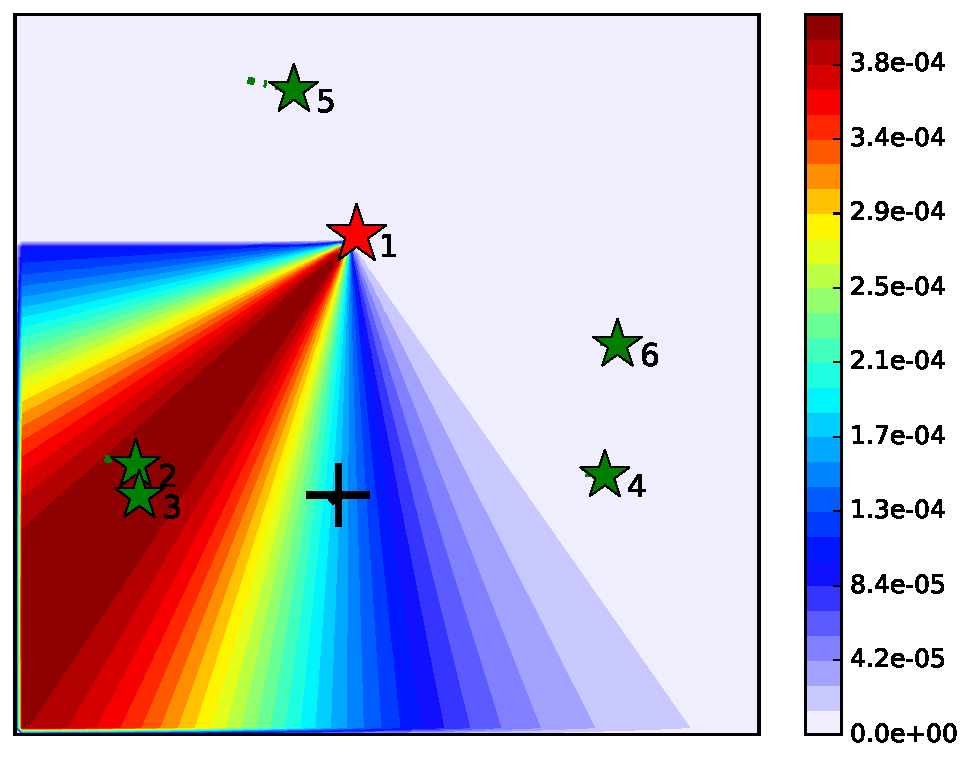
\includegraphics[width=\textwidth]{figures/brg_mov_sen_mov_tar_rbt1_step1}
		\caption{Step 1}\label{fig:mov_sen_mov_tar_sing1}
	\end{subfigure}
	\begin{subfigure}[b]{0.24\textwidth}
		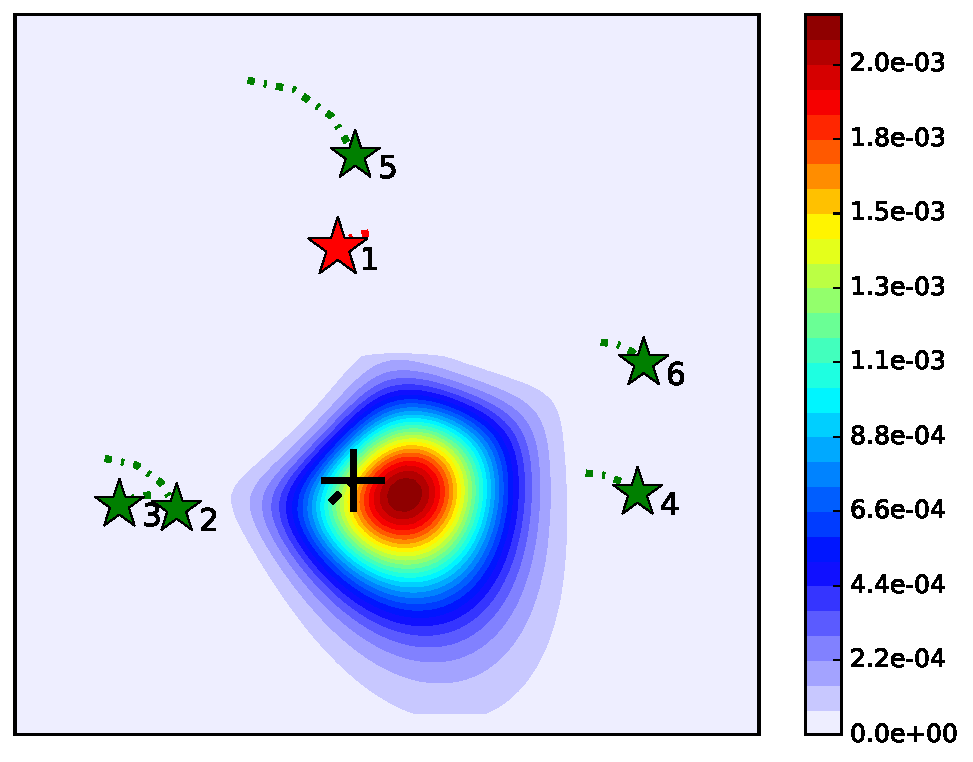
\includegraphics[width=\textwidth]{figures/brg_mov_sen_mov_tar_rbt1_step3}
		\caption{Step 3}\label{fig:mov_sen_mov_tar_sing2}
	\end{subfigure}	
	\begin{subfigure}[b]{0.24\textwidth}
		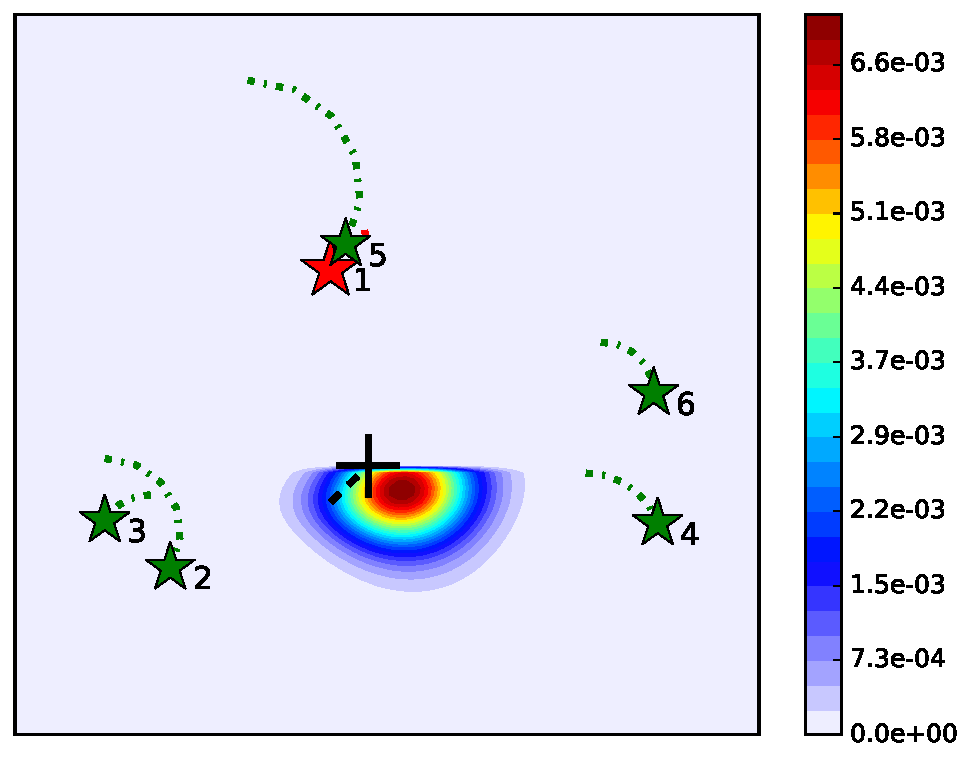
\includegraphics[width=\textwidth]{figures/brg_mov_sen_mov_tar_rbt1_step5}
		\caption{Step 5}\label{fig:mov_sen_mov_tar_sing3}
	\end{subfigure}	
	\begin{subfigure}[b]{0.24\textwidth}
		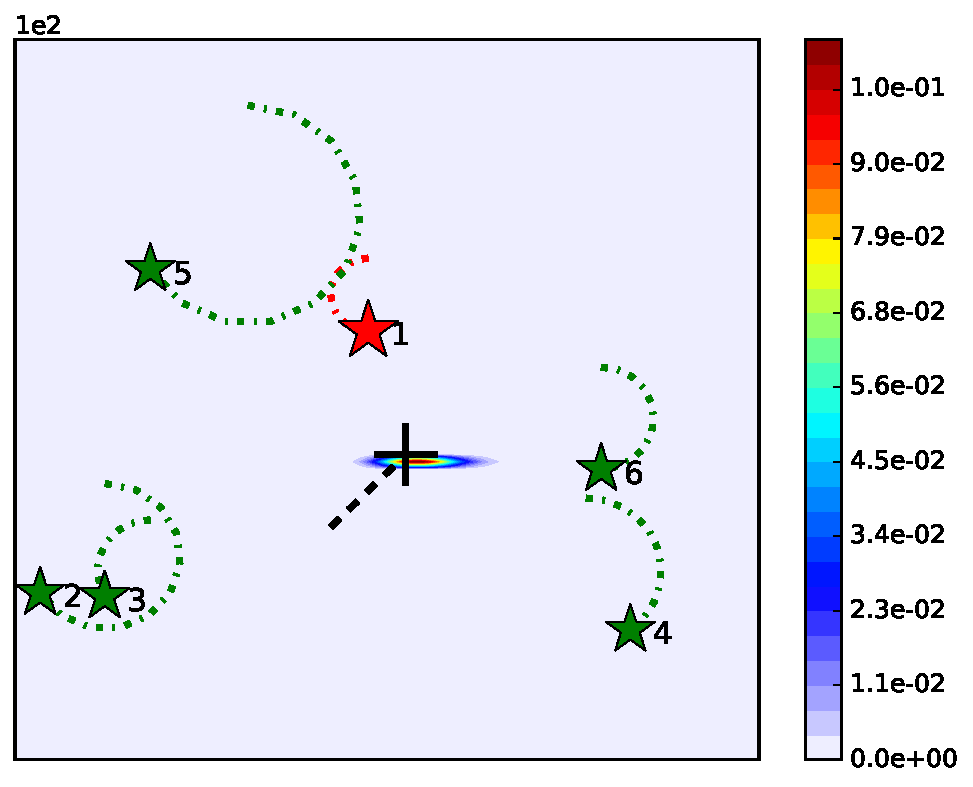
\includegraphics[width=\textwidth]{figures/brg_mov_sen_mov_tar_rbt1_step10}
		\caption{Step 10}\label{fig:mov_sen_mov_tar_sing4}
	\end{subfigure}
	\begin{subfigure}[b]{0.24\textwidth}
		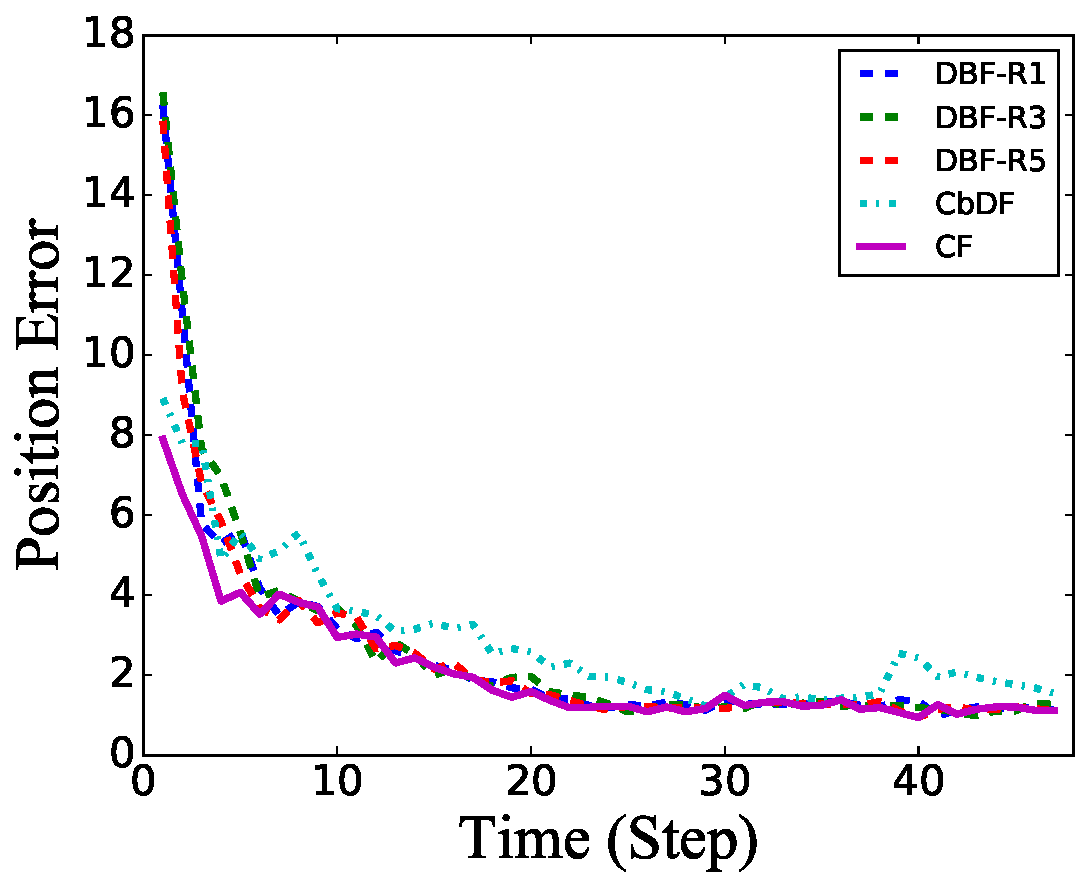
\includegraphics[width=\textwidth]{figures/brg_mov_sen_mov_tar_pos_err.pdf}
		\caption{Position Error}\label{fig:mov_sen_mov_tar_pos_err}
	\end{subfigure}
	\begin{subfigure}[b]{0.24\textwidth}
		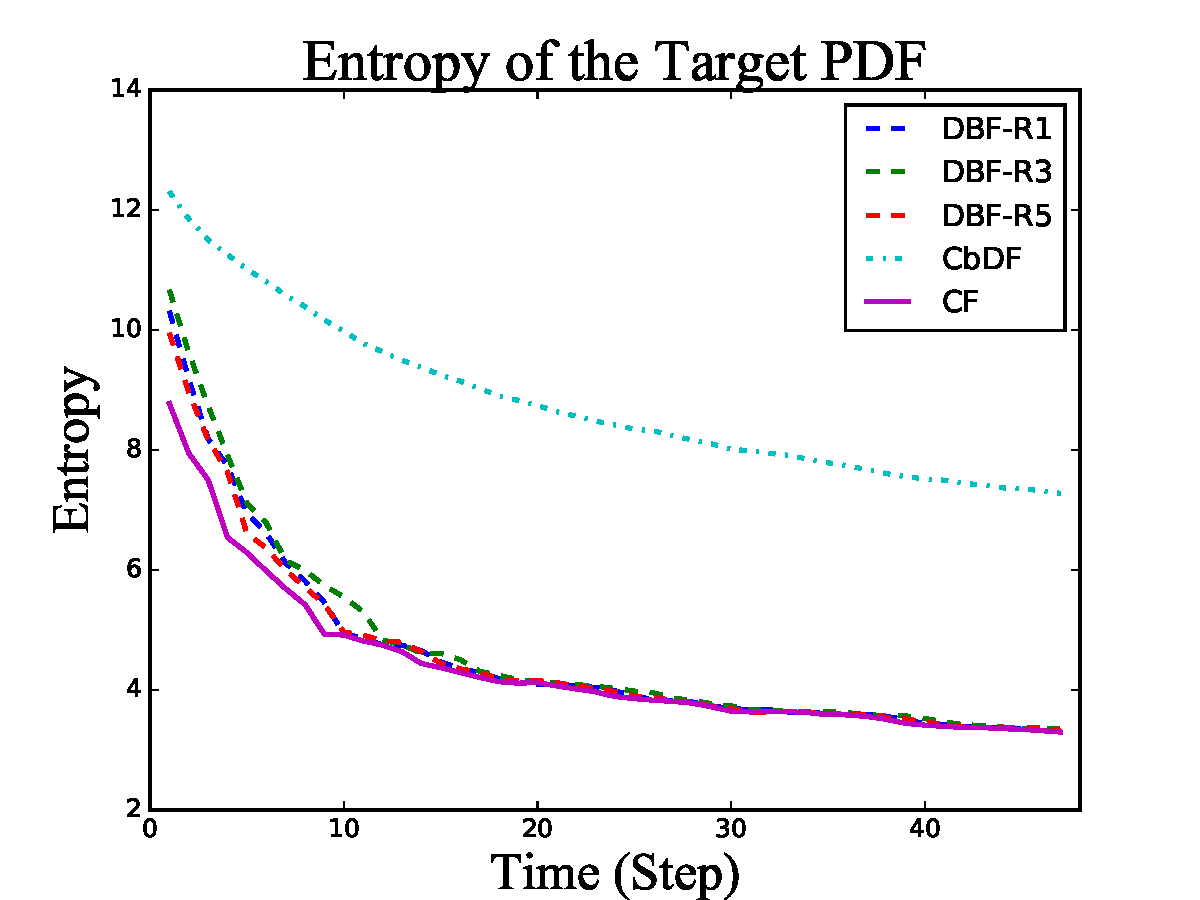
\includegraphics[width=\textwidth]{figures/brg_mov_sen_mov_tar_entropy.pdf}
		\caption{Entropy of Individual PDF}\label{fig:mov_sen_mov_tar_entropy}
	\end{subfigure}
	%	\begin{subfigure}[b]{0.4\textwidth}
	%		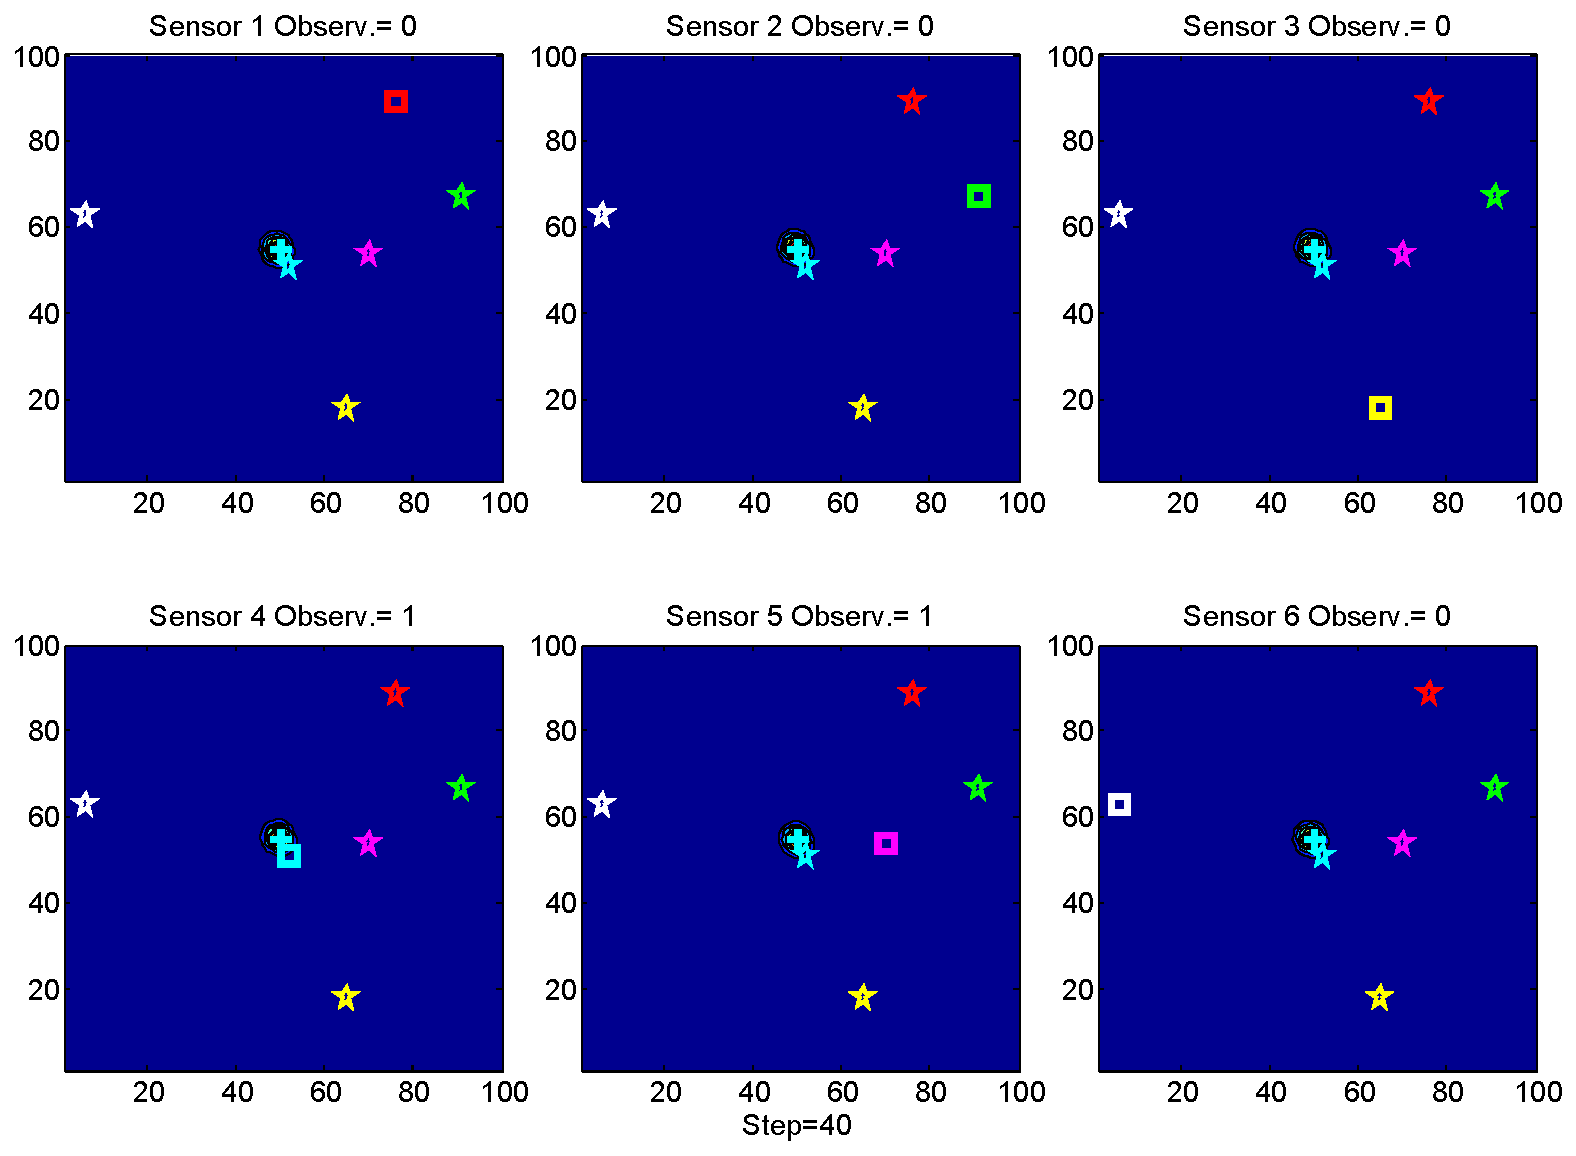
\includegraphics[width=\textwidth]{figures/mov_sen_mov_tar_40}
	%		\caption{Step 40}\label{fig:mov_sen_mov_tar_all}
	%	\end{subfigure}
	\caption{(a)-(d) The $1^\text{st}$ UGV's individual PDFs at different times. The green dashed lines represent robots' trajectories. (e) Average position estimation error. (f) Average entropy of individual PDFs.}
	\label{fig:mov_sen_mov_tar}
	%	\vspace{-1.1em}
\end{figure}

\begin{figure}%[thpb]
	\centering
	\begin{subfigure}[b]{0.24\textwidth}
		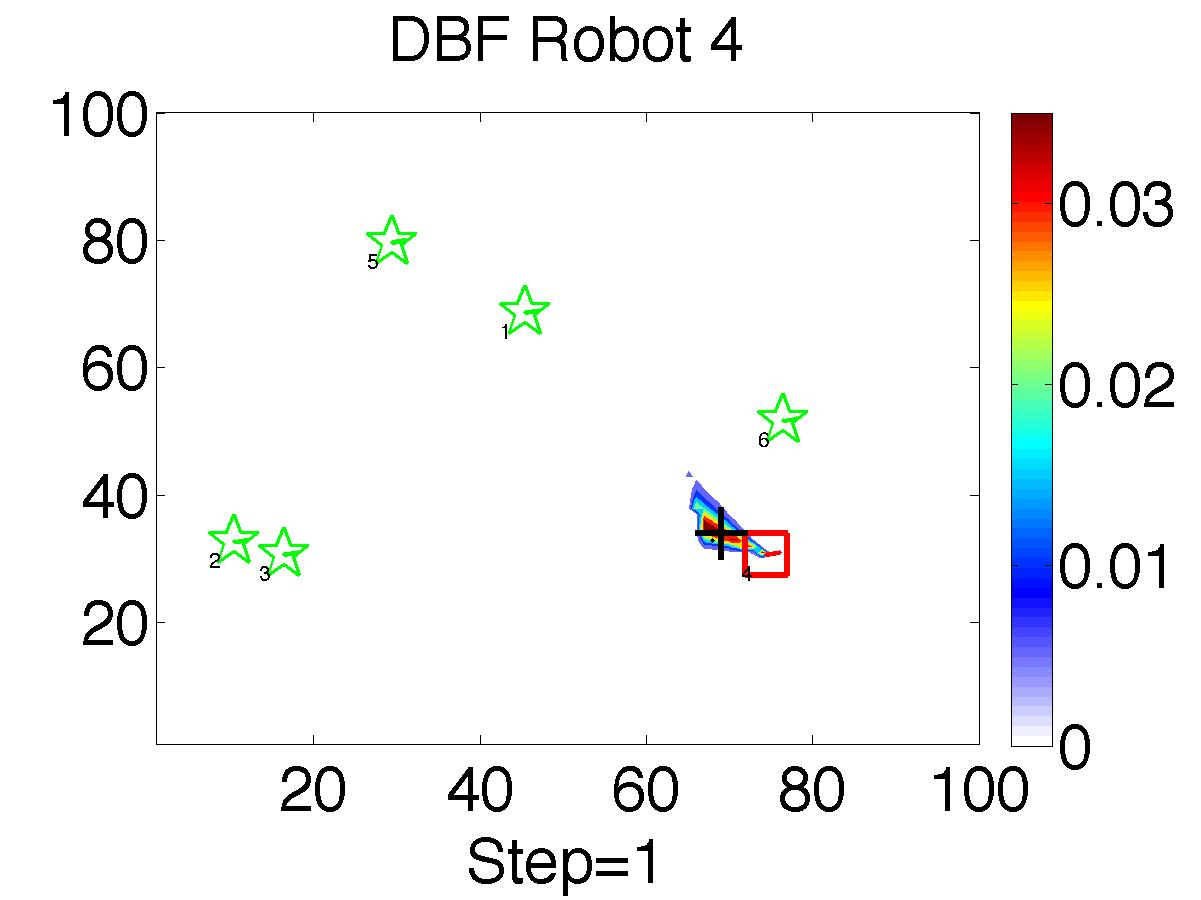
\includegraphics[width=\textwidth]{figures/hetero_mov_sen_mov_tar_rbt4_step1}
		\caption{Step 1}\label{fig:htr_mov_sen_mov_tar_sing1}
	\end{subfigure}
	\begin{subfigure}[b]{0.24\textwidth}
		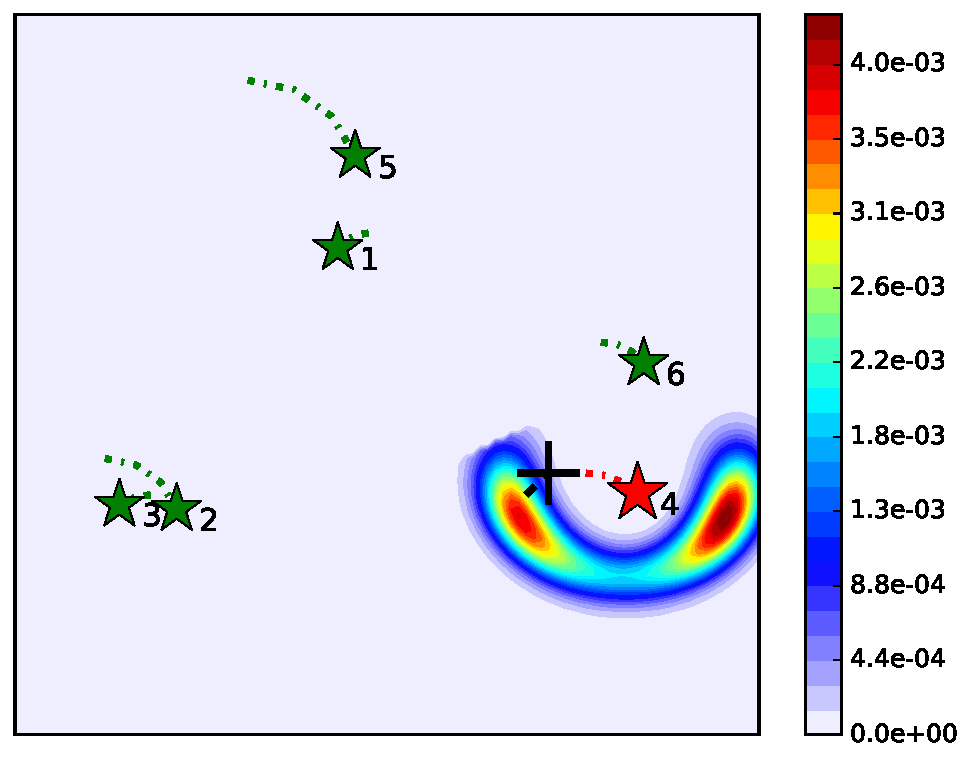
\includegraphics[width=\textwidth]{figures/hetero_mov_sen_mov_tar_rbt4_step3}
		\caption{Step 3}\label{fig:htr_mov_sen_mov_tar_sing2}
	\end{subfigure}
	\begin{subfigure}[b]{0.24\textwidth}
		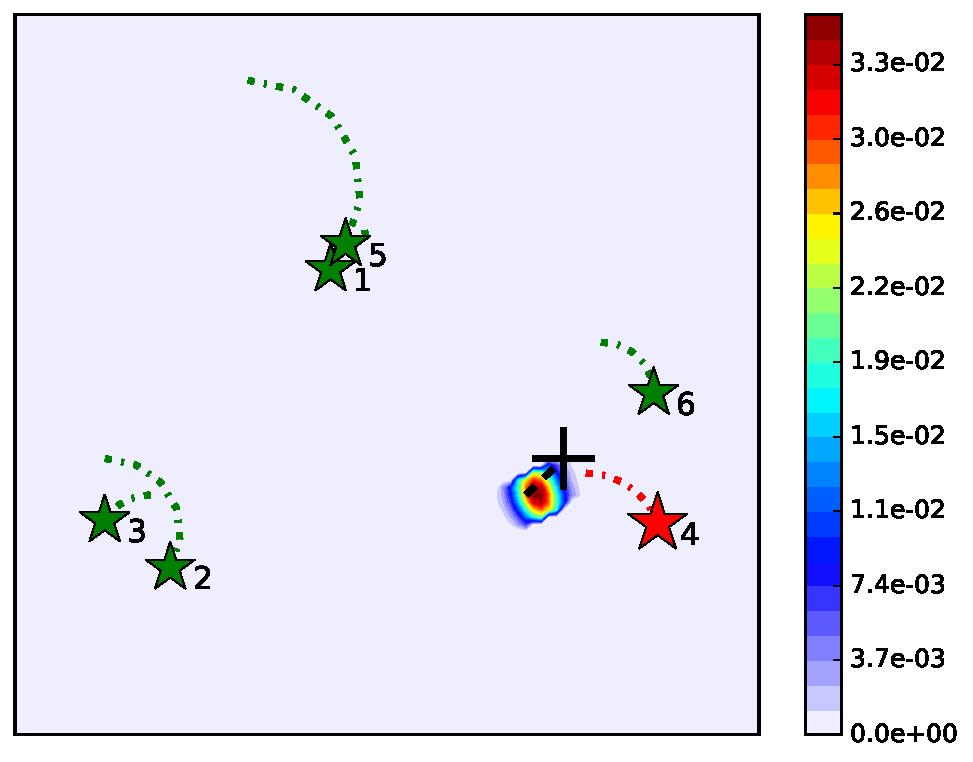
\includegraphics[width=\textwidth]{figures/hetero_mov_sen_mov_tar_rbt4_step5}
		\caption{Step 5}\label{fig:htr_mov_sen_mov_tar_sing3}
	\end{subfigure}
	\begin{subfigure}[b]{0.24\textwidth}
		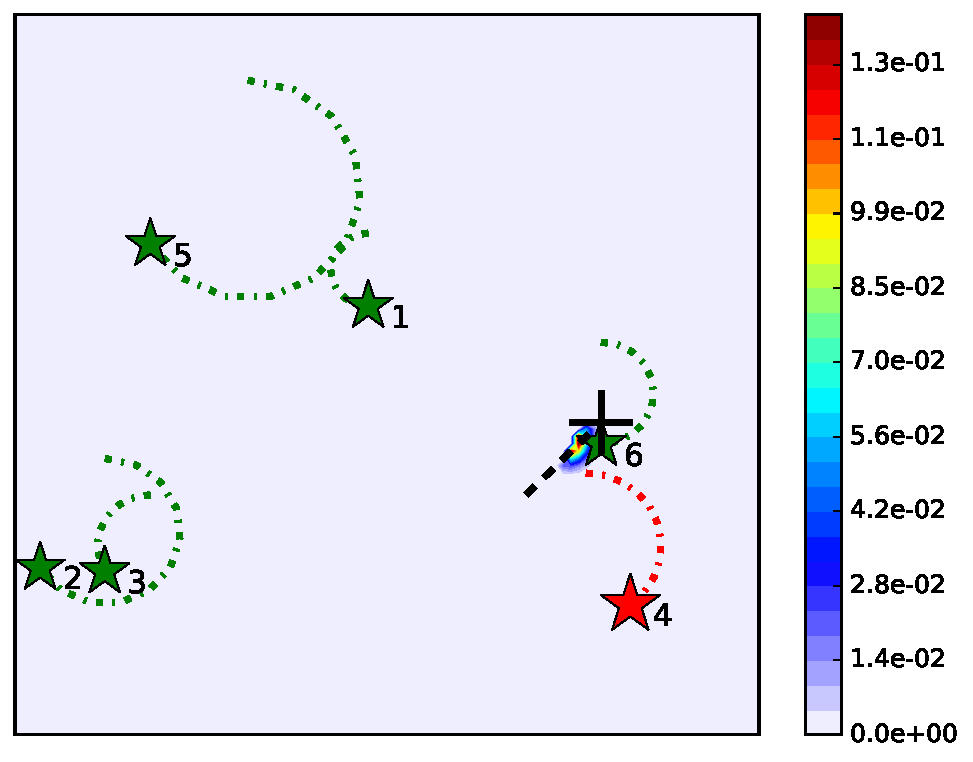
\includegraphics[width=\textwidth]{figures/hetero_mov_sen_mov_tar_rbt4_step10}
		\caption{Step 10}\label{fig:htr_mov_sen_mov_tar_sing4}
	\end{subfigure}
	\begin{subfigure}[b]{0.24\textwidth}
		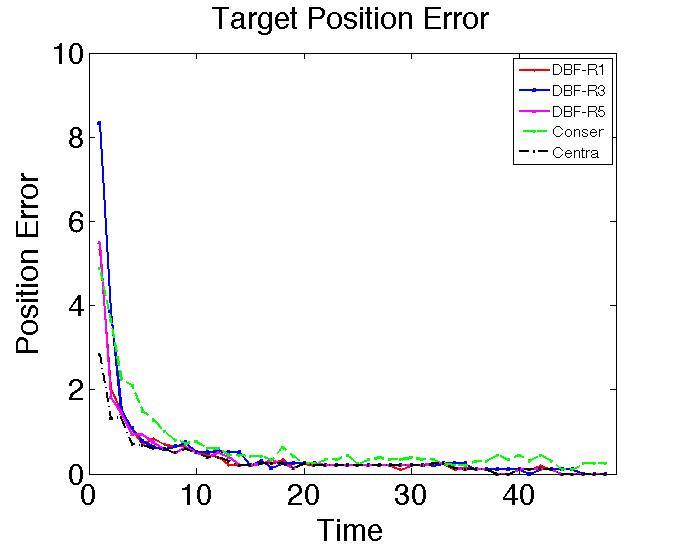
\includegraphics[width=\textwidth]{figures/hetero_mov_sen_mov_tar_pos_err}
		\caption{Position Error}\label{fig:htr_mov_sen_mov_tar_pos_err}
	\end{subfigure}
	\begin{subfigure}[b]{0.24\textwidth}
		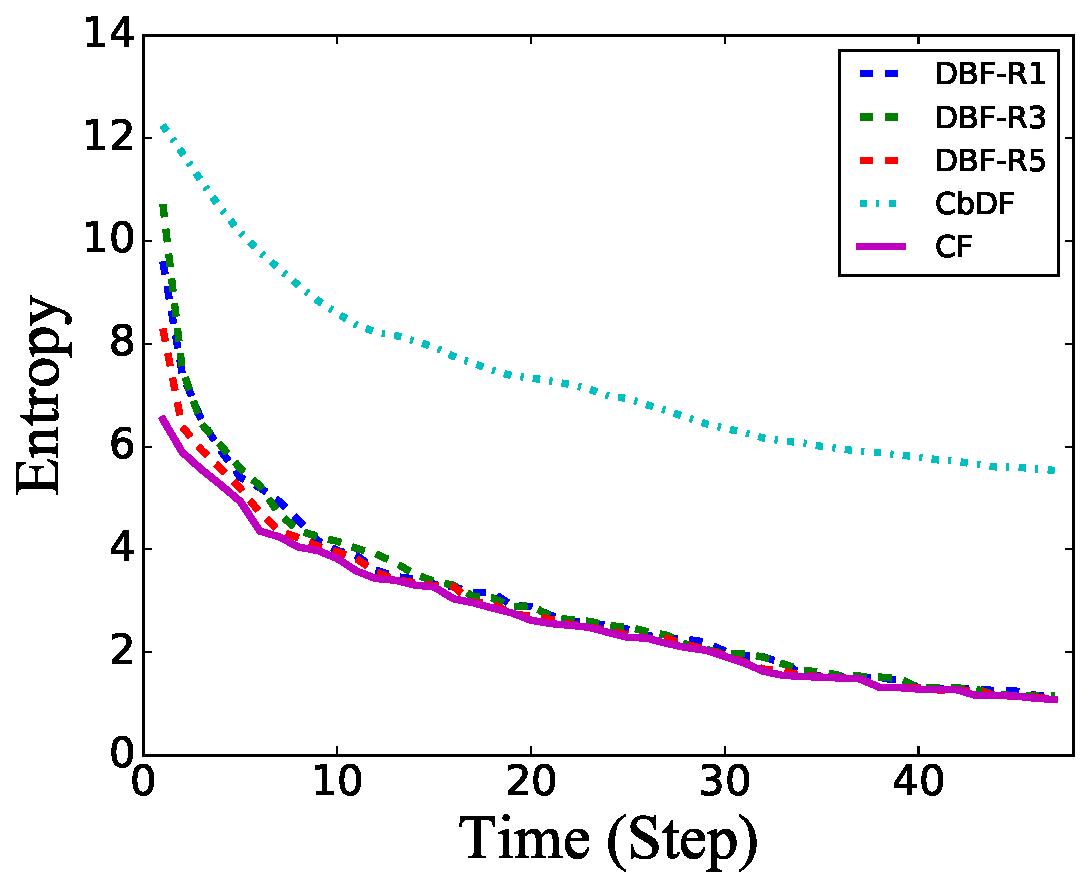
\includegraphics[width=\textwidth]{figures/hetero_mov_sen_mov_tar_entropy}
		\caption{Entropy of Individual PDF}\label{fig:htr_mov_sen_mov_tar_entropy}
	\end{subfigure}
	\caption{(a)-(d) The $4^\text{th}$ UGV's individual PDF at different times. (e) Average position estimation error. (f) Average entropy of individual PDFs.}
	%\label{fig:sta_sen_sta_tar}
	%	\vspace{-1.2em}
\end{figure}

Simulation has been conducted to evaluate the effectiveness of LIFO-DBF for target localization using a team of six UGVs.
%In all scenarios, each UGV is equipped with a binary sensor. 
The networked UGVs take a ring communication topology that each UGV can communicate with two fixed neighbors.
%The probabilistic sensor model
% \cref{eqn:bin_sensor1,eqn:bin_sensor0}, 
%takes the form defined in \Cref{eqn:gauss_sensor}.
%\small\begin{align}\label{eqn:gauss_sensor}
%\small\begin{subequations}\label{eqn:gauss_sensor}
%	\begin{align}
%		P(z^i_k=1|x_k^g;x_k^i)&=e^{-\frac{1}{2}(x_k^g-x_k^i)^T{\Sigma}^{-1}(x_k^g-x_k^i)}\\
%%		\exp\left\lbrace -\frac{1}{2}(x-x^R)^T{\Sigma}^{-1}(x-x^R)\right\rbrace \\
%		P(z^i_k=0|x_k^g;x_k^i)&=1-P(z^i_k=1|x_k^g;x_k^i),
%	\end{align}
%\end{subequations}\normalsize
%which reflects the fact that target detection becomes more probable as the UGV approaches the target position.
%\end{align}\normalsize
%where $x^s$ denotes the UGV position where current measurement is obtained. 
%Figure 4 shows the 1-D illustration of Gaussian binary sensor model.
%where $x^R$ denotes the UGV position, which is included in UGV state $y^R$.
DBF is implemented using the histogram filter method, by which the continuous space is finely discretized into finitely many regions and the individual PDF is approximated by the cumulative probability of each region \cite{thrun2005probabilistic}. 
%Other approaches, such as particle filters \cite{}, can also be used.
Two types of scenarios are used: in the first scenario, both UGVs and the target are static;
%, which acts as a proof of concept of LIFO-DBF for static target.
the second scenario subsequently deals with moving UGVs for localizing a moving target. 
In each scenario, we also test two different kinds of UGV team: the first UGV team, called the homogeneous team, is equipped with bearing-only sensors; in the second team, called the heterogeneous team, three UGVs are equipped with bearing-only sensor and the other three equipped with range-only sensors.
The bearing-only sensors are assumed to have large enough sensing range to cover the simulation field and the measurement noise is a zero-mean Gaussian white noise with standard deviation being $0.5$.
The range-only sensors are assumed to have $360\degree$ field of view and the measurement noise is a zero-mean Gaussian white noise with standard deviation being $5$.
%When the target is outside of the sensor's sensing range, an empty measurement is obtained, which is also used for updating the individual PDF.

In both scenarios, LIFO-DBF is compared with two commonly adopted approaches in multi-agent filtering: the consensus-based distributed filtering (CbDF) method \cite{olfati2006belief} and the centralized filtering (CF) method \cite{veeravalli2012distributed}.
The CbDF requires UGVs to continually exchange their individual PDFs with direct neighbors, computing the average of its own and the received PDFs. 
Multiple rounds of communication and averaging are conducted during the ``Sending Step'' and ``Receiving Step'' in \Cref{alg:lifo} at each step to ensure the convergence of UGV's individual PDFs.
The CF assumes a central unit that can constantly receive and fuse all UGVs' latest measurements into a single PDF.
Ten test trials with randomly generated initial UGV and target positions are run and each trial is terminated after 50 time steps.
The average error between the estimated (using the MAP estimator) and true target position and the average entropy of individual PDFs of all 10 trials using these three approaches are compared.


\subsection{Static UGVs, Static Target}
%In this test, all UGVs are equipped with bearing-only sensors.\label{subsec:sim1}
The individual PDF of each UGV is initialized as a uniform distribution over a bounded space. 
At each time step, each UGV executes the LIFO-DBF for static target (\Cref{subsec:LIFO-dbf-sta-tar}) to update their estimation of target position.
The evolution of the $1^\text{st}$ robot's individual PDF is shown in \Cref{fig:sta_sen_sta_tar_sing1,fig:sta_sen_sta_tar_sing2,fig:sta_sen_sta_tar_sing3,fig:sta_sen_sta_tar_sing4}. 
Since the robot is equipped with a noisy bearing-only sensor, the measurement at step $1$ results in a wide distribution with the peak centered along the noise-corrupted measured direction from the sensor to the target, as \Cref{fig:sta_sen_sta_tar_sing1} illustrates.
%six static UGVs, as represented by green stars and red square in , are placed in the field.
%The target is also assumed to be static, with $A$ being an identity matrix and $B_k$ being a zero matrix in \cref{eqn:tar_motion_model}.
% shows a test trial when both the UGVs and the target are static. %of the positions of six static UGVs are shown as stars and square.
%Due to space constraint, only the individual PDF of the first UGV is shown.
%The individual PDF of the first UGV at different time steps are shown in \cref{fig:sta_sen_sta_tar_sing1,fig:sta_sen_sta_tar_sing2,fig:sta_sen_sta_tar_sing3,fig:sta_sen_sta_tar_sing4}.
%Each UGV constantly receives binary measurements of the target.
%The LIFO-DBF for static target is implemented on each UGV for target localization.
%The networked UGVs use a ring communication topology that each UGV can communicate with two fixed neighbors.
%\cref{fig:sta_sen_sta_tar} shows the estimation results of the static target. 
%After the initial measurement, each UGV forms a circular individual PDF, centered at its own position.
%\cref{fig:sta_sen_sta_tar_sing1} shows the individual PDF after initial measurement for $1^\text{st}$ UGV.
%The circular PDF happens because the Gaussian sensor model (\Cref{eqn:gauss_sensor}) only depends on the distance between UGV and target.
As more measurements are fused, the individual PDF asymptotically concentrates to the true location of the target, which accords with the consistency of LIFO-DBF.
%In fact, with the Guassian sensor model (\Cref{eqn:gauss_sensor}), all positions with equal distance to a UGV belong to the same equi-parameter set of the UGV.
%Considering the system of six UGVs located separately, the equi-parameter set that contains the actual target position only contains one element.
%\cref{fig:entropy} (a) shows the decrease of the entropy of each UGV's individual PDF, indicating the reduction of the uncertainty in PDF estimation.

The \Cref{fig:sta_sen_sta_tar_pos_err,fig:sta_sen_sta_tar_entropy} shows the comparison of LIFO-DBF with CbDF and CF.
Unsurprisingly, the CF achieves the best performance in terms of both small position estimation error and fast reduction of entropy. 
This happens because the central unit has access to the latest measurements of all UGVs, thus being able to make the most use of all available information.
It is worth noting that, LIFO-DBF achieves similar asymptotic performance as the CF, both in position estimation error and entropy reduction; this is achieved even though each UGV only communicates with its two neighboring UGVs, which requires less communication burden than the CF.
The CbDF has the worst performance among these three filtering approaches. 
It results in slow reduction of entropy and the position error remains large.
This happens because Bayes filtering (\Cref{eqn:bayes_pred,eqn:bayes_upd}) is a nonlinear process.
Using the linear average consensus law to fuse individual PDFs thus deviates from the actual Bayesian filtering and therefore cannot fully exploit the information of new measurements to reduce the uncertainty of estimation.

The \Cref{fig:htr_sta_sen_sta_tar} shows the simulation results of the heterogeneous team.
The individual PDF of the UGV with a noisy range-only sensor is presented in \Cref{fig:htr_sta_sen_sta_tar_sing1,fig:htr_sta_sen_sta_tar_sing2,fig:htr_sta_sen_sta_tar_sing3,fig:htr_sta_sen_sta_tar_sing4}.
At step $1$, the target is detected and the individual PDF is updated such that the peak of the  distribution centers at the positions whose distance to the sensor equals the noise-corrupted measured value. 
Similar to the case of using the homogeneous team, the individual PDF asymptotically concentrates to the true target position.
Due to the use of various sensors, the estimation accuracy increases faster than the homogeneous team case, as shown in \Cref{fig:htr_sta_sen_sta_tar_pos_err,fig:htr_sta_sen_sta_tar_entropy}.
It can also be noticed that, LIFO-DBF achieves similar performance as CF, while the performance of CbDF is the worst.

\begin{figure}
	\centering
	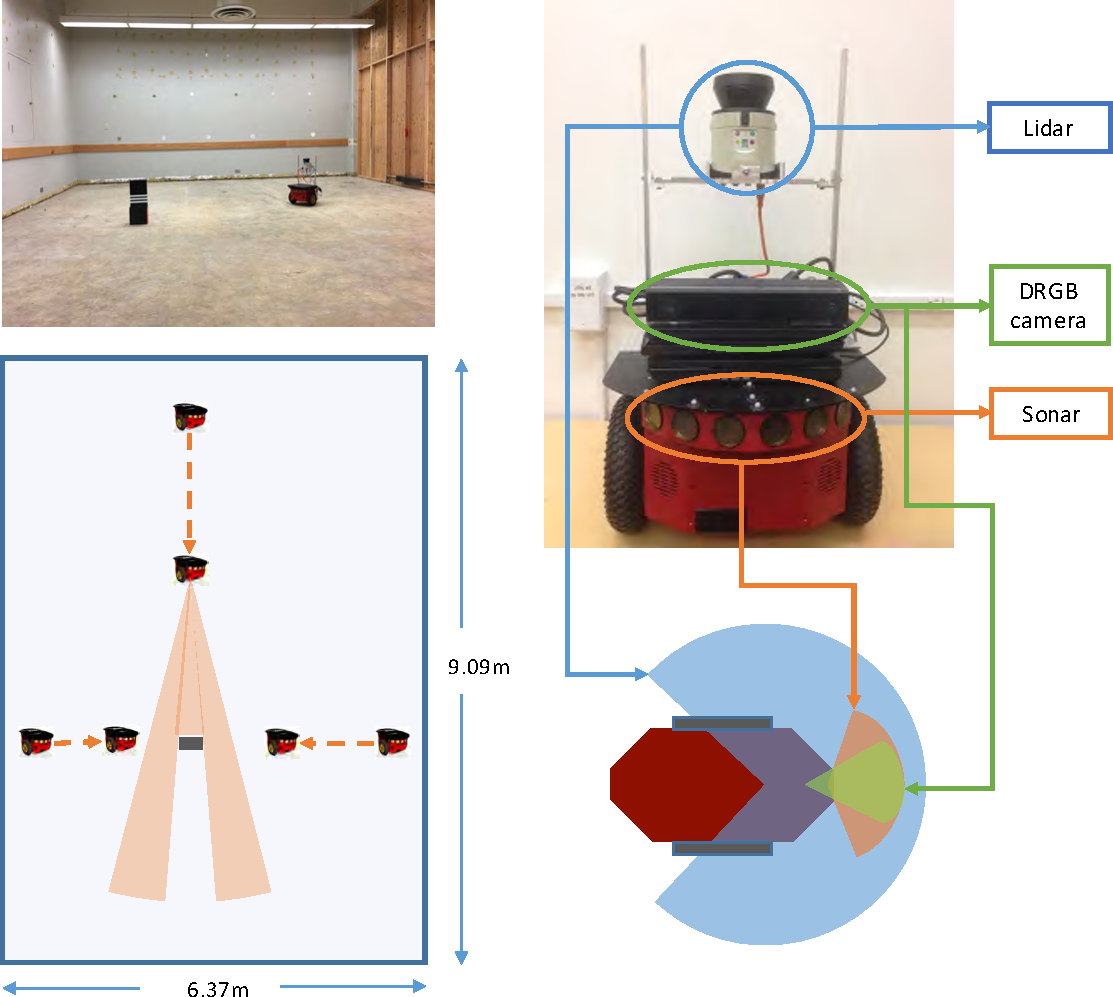
\includegraphics[width=0.47\textwidth]{figures/exp_setup_rdsize}
	\caption{Experiment Setup. Left: Three robots are used for localizing the target (black box). The room size is $9.09m\times 6.37m$. The orange sectors show the sonar sensing domain. Red dashed lines show the trajectory of each robot. Right: The mobile robot platform is equipped with different sensors. The sonar sensor is used for target localization.}\label{fig:exp_scene}
\end{figure}

\subsection{Moving UGVs, Moving Target}
In this scenario, each UGV follows a pre-defined circular trajectory. 
The target motion is modeled as a single-integrator with unit velocity on both directions.
Each UGV executes the LIFO-DBF for moving target (\cref{subsec:LIFO-dbf-mov-tar}) for estimation.
\Cref{fig:mov_sen_mov_tar_sing1,fig:mov_sen_mov_tar_sing2,fig:mov_sen_mov_tar_sing3,fig:mov_sen_mov_tar_sing4} and \Cref{fig:htr_mov_sen_mov_tar_sing1,fig:htr_mov_sen_mov_tar_sing2,fig:htr_mov_sen_mov_tar_sing3,fig:htr_mov_sen_mov_tar_sing4} illustrate the evolution of individual PDF for homogeneous and heterogeneous teams, respectively.
They all present similar asymptotic behavior of individual PDFs as in aforementioned simulations.
%Note that \Cref{fig:htr_mov_sen_mov_tar_sing1} shows the individual PDF at step $1$ when the target is out of the sensing domain of the $5^\text{th}$ UGV's range-only sensor.
%It can be noticed that the individual PDF concentrates to the true target location when the target constantly moves.

\cref{fig:mov_sen_mov_tar_pos_err,fig:mov_sen_mov_tar_entropy} and \cref{fig:htr_mov_sen_mov_tar_pos_err,fig:htr_mov_sen_mov_tar_entropy} compare LIFO-DBF with CbDF and CF.
%Similar to results in \cref{subsec:sim1}, CF achieves best performance with smallest position estimation error and fastest entropy reduction; LIFO-DBF shows similar asymptotic performance as the CF; and
%CbDF has the slowest entropy reduction among all three filtering approaches.
It is worth noting that, for the heterogeneous team, CbDF achieves comparable position estimation error performance as the CF and LIFO-DBF.
%This is not an unexpected result: due to the consensus procedure, CbDF is able to fuse the latest individual PDFs of each UGV via the averaging process. 
%This is especially useful when the environment is dynamically changing.
%In contrast, LIFO-DBF for each UGV only uses delayed information from neighboring UGVs, thus gaining less knowledge about the target's current position.
However, CbDF requires multiple rounds of exchanging individual PDFs, which incurs much higher communication burden than LIFO-DBF at each time step.
Considering the small difference in position estimation error and significantly faster entropy reduction, LIFO-DBF is still preferable over CbDF for moving target scenario.

\section{Indoor Experiment using Mobile Robot}\label{sec:exp}


\begin{figure}
	\centering
	\begin{subfigure}[b]{0.24\textwidth}
		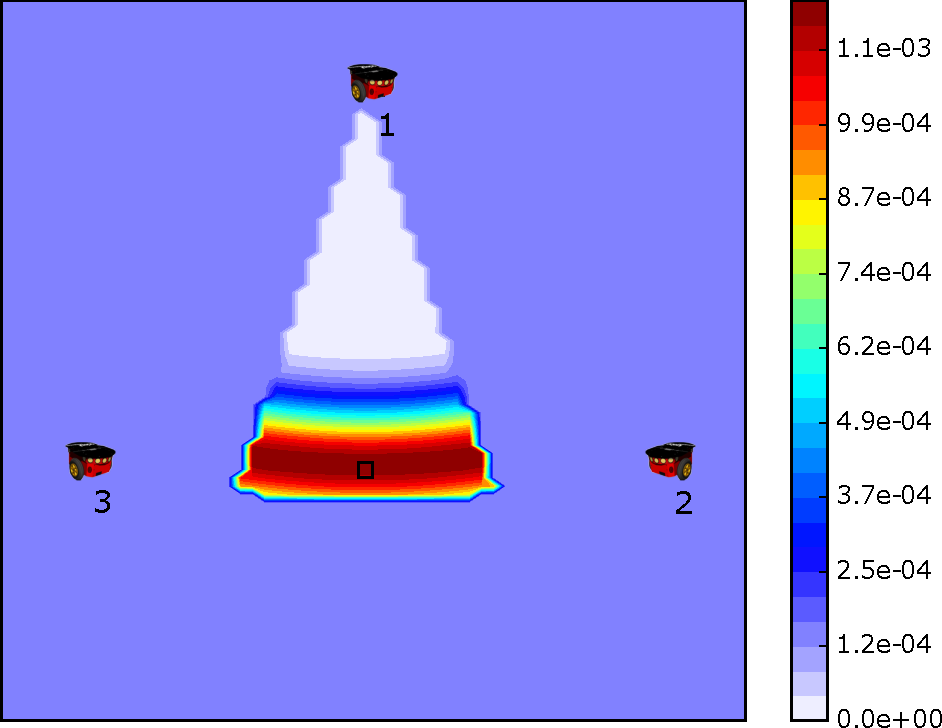
\includegraphics[width=\textwidth]{figures/sonar_mov_sen_sta_tar_rbt1_step1}
		\caption{Step 1}\label{fig:sonar_mov_sen_sta_tar_rbt1_step1}
	\end{subfigure}
	\begin{subfigure}[b]{0.24\textwidth}
		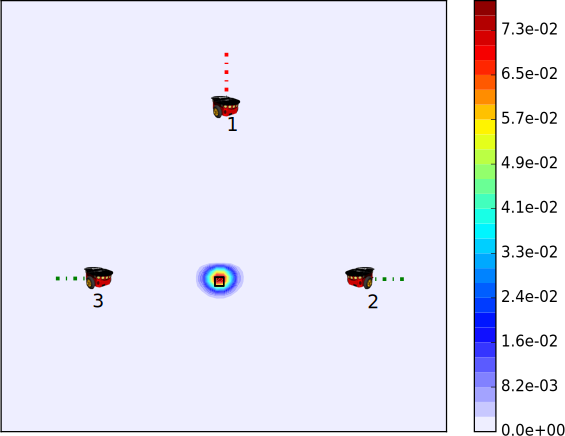
\includegraphics[width=\textwidth]{figures/sonar_mov_sen_sta_tar_rbt1_step10}
		\caption{Step 10}\label{fig:sonar_mov_sen_sta_tar_rbt1_step10}
	\end{subfigure}	
	\begin{subfigure}[b]{0.24\textwidth}
		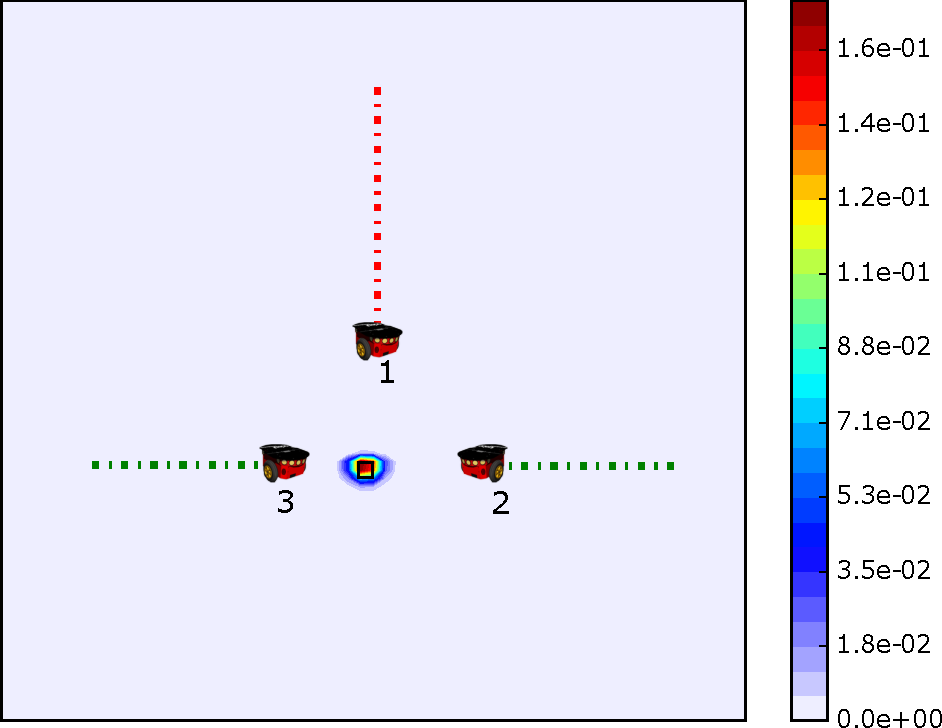
\includegraphics[width=\textwidth]{figures/sonar_mov_sen_sta_tar_rbt1_step20}
		\caption{Step 20}\label{fig:sonar_mov_sen_sta_tar_rbt1_step20}
	\end{subfigure}	
	\begin{subfigure}[b]{0.24\textwidth}
		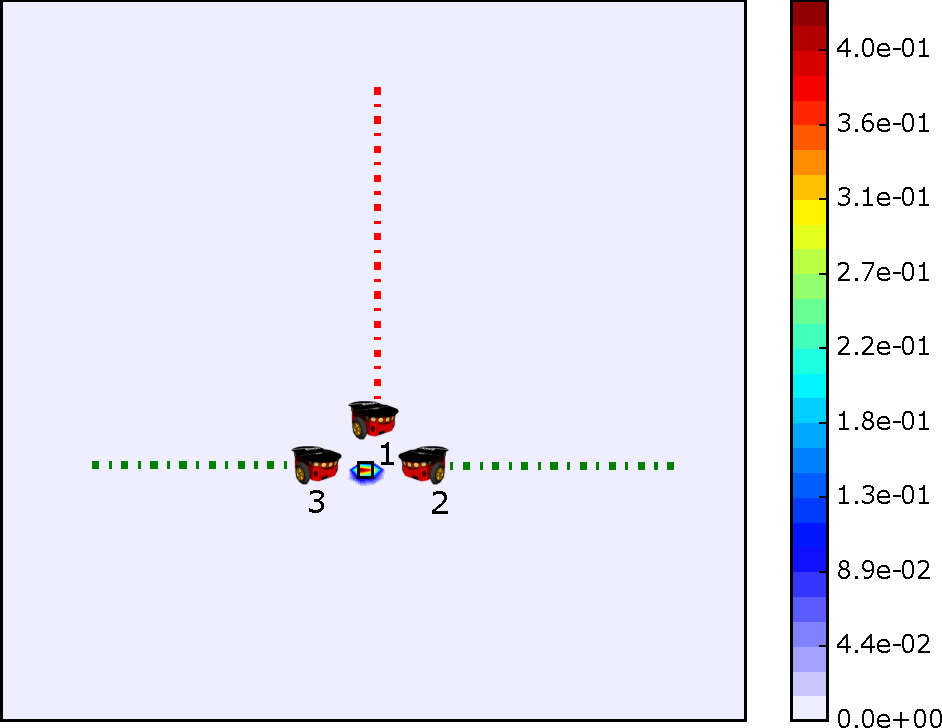
\includegraphics[width=\textwidth]{figures/sonar_mov_sen_sta_tar_rbt1_step30}
		\caption{Step 30}\label{fig:sonar_mov_sen_sta_tar_rbt1_step30}
	\end{subfigure}	
	\caption{The $1^\text{st}$ robot's individual PDF at different time steps.}
\end{figure}


%\begin{figure}
%	\centering
%	\begin{subfigure}[b]{0.24\textwidth}
%		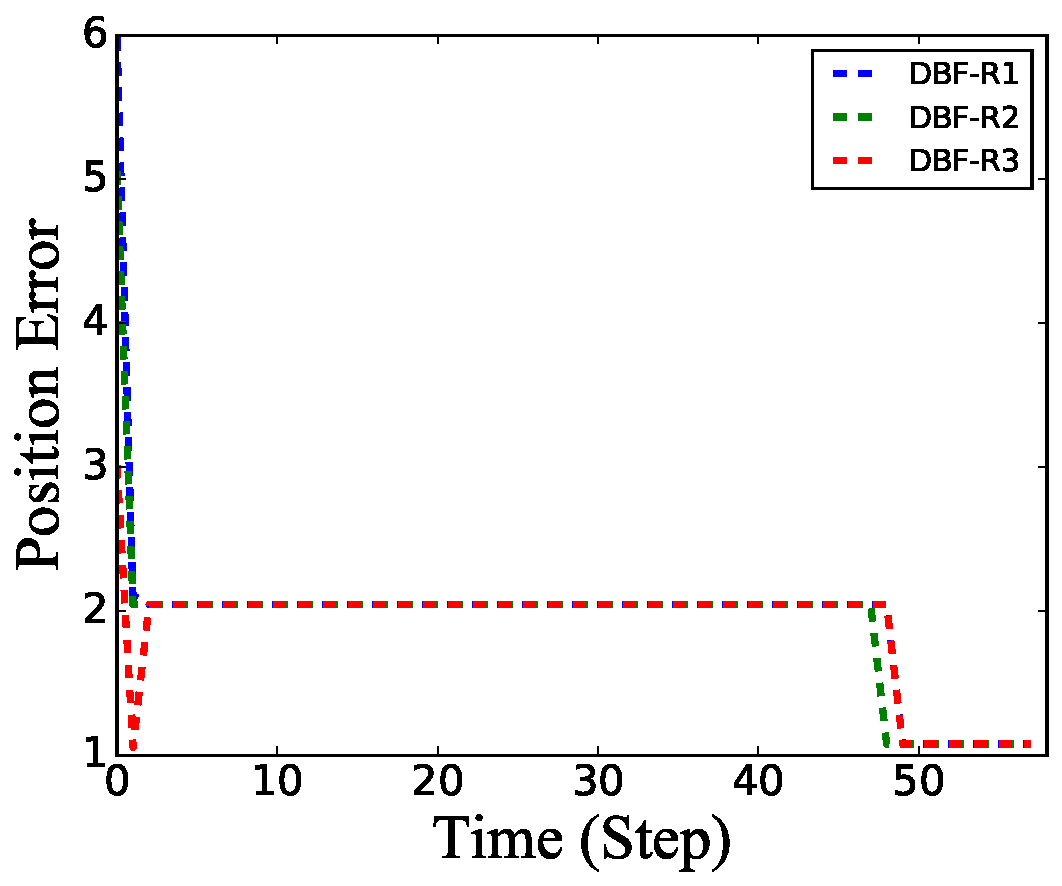
\includegraphics[width=\textwidth]{figures/sonar_pos_err}
%		\caption{Position Error}\label{fig:sonar_pos_err}
%	\end{subfigure}
%	\begin{subfigure}[b]{0.24\textwidth}
%		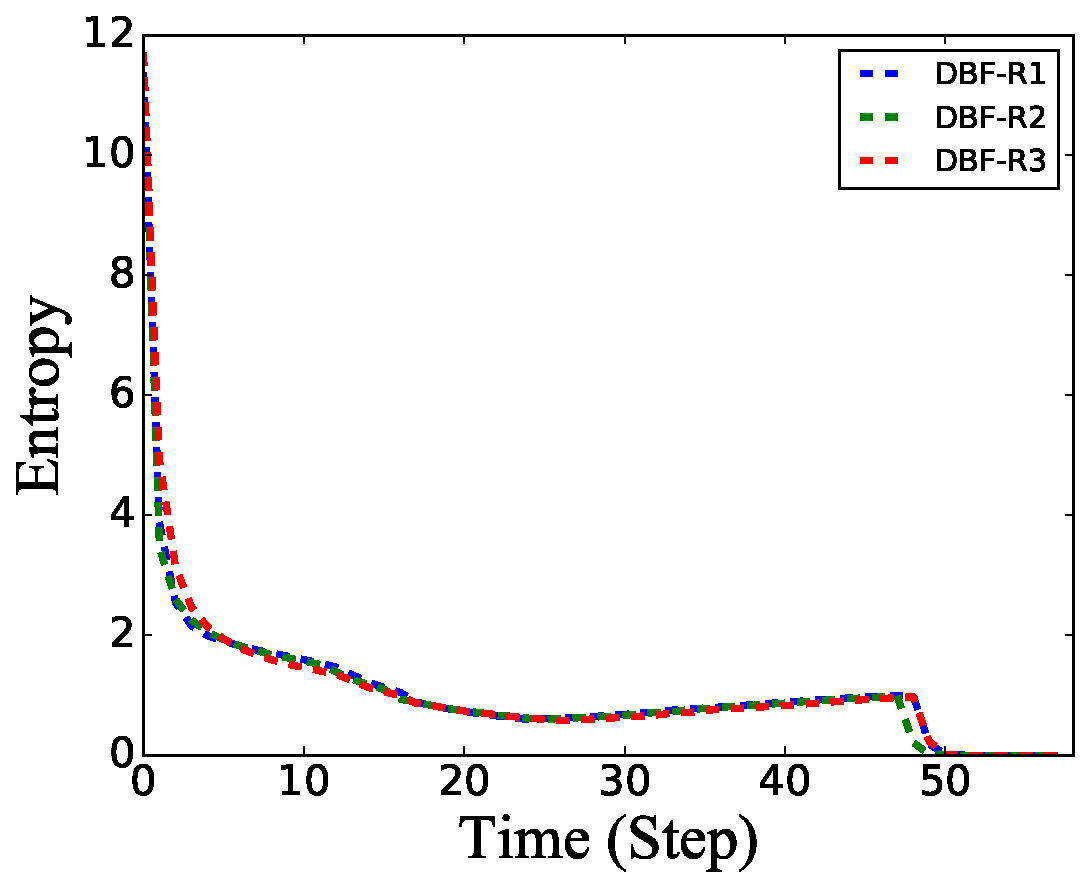
\includegraphics[width=\textwidth]{figures/sonar_entropy}
%		\caption{Entropy of Individual PDF}\label{fig:sonar_entropy}
%	\end{subfigure}	
%	\caption{Estimation position error and entropy for three robots in the experiment.}
%\end{figure}
We have conducted a target localization experiment to validate the LIFO-DBF approach in an indoor environment.
The experiment equipments and environment is illustrated in \Cref{fig:exp_scene}.
%The robot platform is equipped with Lidar, camera and sonar sensors.
%In this experiment, we only utilize the sonar sensors for localization, since they has less measurement accuracy than other two types of sensors, which provides an effective testbed for evaluating the proposed method. 
%using sonar sensors mounted on a P3DX robot platform for localizing a static target (\Cref{fig:exp_scene}).
The sonar sensor on the mobile robot is used for target localization and the sonar has the sensing field of view of $25\degree$ and the range of $4.9m$.
Its measurement noise is modeled as a zero-mean Gaussian random variable with standard deviation $0.5m$.
%The experiment is conducted in an indoor environment and 
The probability map is constructed on a grid that is evenly separated with $0.1m$ interval on each axis.
%To avoid the inaccuracy caused by sensor state measurement, 
We manually measure the sensor positions at which the measurements are obtained. % for estimating the target position.
%Due to the limited robot platform, we collect the sensor measurement from different positions and postprocess these data, treating them as the data from three different robots.
%We use 
A small cardboard box is used as the target and the effect of the target size has been compensated during the postprocessing of the measurement data.

\Cref{fig:sonar_mov_sen_sta_tar_rbt1_step1,fig:sonar_mov_sen_sta_tar_rbt1_step10,fig:sonar_mov_sen_sta_tar_rbt1_step20,fig:sonar_mov_sen_sta_tar_rbt1_step30} show the evolution of the $1^\text{st}$ robot's individual PDF.
At step $1$, the probability mass concentrates to a narrow band due to the fact that the sonar sensor used in this experiment has limited FOV and noise in range measurement.
As new measurements from different robots are continually fused, the probability mass gradually concentrates to the true position of the target. 
This validates the consistency of LIFO-DBF and demonstrates its effectiveness for distributed filtering.
%Experiment results show fast convergence between the MAP estimate of target position to the true position value (\Cref{fig:sonar_pos_err,fig:sonar_entropy}).
%\Cref{} illustrates the entropy reduction over time.
%In the end, entropy reduces to zero and this corresponds to the case that all probability mass concentrates to the small cell that contains the target.
%The sudden drop of the entropy at step $48$ is because the sensor comes closer to the target and obtains a more accurate measurement of the target.
%Experiment results have shown the effectiveness of the LIFO-DBF for target localization.


\section{CONCLUSION}\label{sec:conclu}
This paper presents a measurement dissemination-based distributed Bayesian filtering (DBF) approach for a multi-UGV network, utilizing the Latest-In-and-Full-Out (LIFO) protocol for measurement exchange.
%Different from statistics dissemination approaches that transmit posterior distributions or likelihood functions, each UGV under LIFO only exchanges with neighboring UGVs a full communication buffer consisting of latest available measurements,
%which significantly reduces the transmission burden between each pair of UGVs from the order of environmental size to that of UGV number.
%Under the condition of fixed and undirected topology, LIFO can guarantee non-intermittent dissemination of all measurements over the network within finite time via local communication among direct neighborhood.
By communicating the communication buffers among neighboring UGVs, LIFO significantly reduces the transmission burden between each pair of UGVs to scale linearly with the network size.
%, with each UGV non-intermittently receiving measurements of all others.
Two types of LIFO-DBF algorithms are proposed to estimate individual PDFs for static target and moving target, respectively. 
%For the static target, each UGV locally fuses the newly received measurements while for the moving target, a record set of historical measurements is stored and updated. 
The consistency of LIFO-DBF is proved by utilizing the law of large numbers, which ensures that the estimated target position converges in probability to the true target position.
The LIFO-DBF is compared with the consensus filter and the centralized filter in various simulations.
Results have shown that LIFO-DBF achieves very similar performance as the centralized filter and is advantageous over the consensus filter.
An experiment is also conducted and has demonstrated the effectiveness of LIFO-DBF for distributed filtering.
% when the number of measurements tends to infinity.
%the agreement between UGVs' estimated target position and the actual position.
%The effectiveness of this method is demonstrated by simulations.

%In this study, we proposed the Latest-In-and-Full-Out (LIFO) strategy for distributed Bayesian filters (LIFO-DBF) in a multi-UGV network.
%% with the application of distributed search and tracking (SAT) of target.
%With fixed communication topology, LIFO guarantees the global dissemination of all UGVs' measurements over the network only via local exchange of measurements among neighbors.
%Once elements in communication buffer (CB) gets filled, each UGV can receive and update its CB non-intermittently under LIFO.
%Two LIFO-DBFs are proposed for SAT of a static and a moving target, respectively. 
%For the static target, each UGV locally fuses the latest knowledge of all UGVs' measurements by only considering the updating step of the Bayesian filter. 
%For the moving target, each UGV maintains a triangle matrix of historical measurements and an iterative Bayesian filtering procedure is applied that alternates between prediction and updating steps upon obtaining the latest available measurements of all UGVs. 
%The consistency of LIFO-DBF is proved by showing the asymptotic concentration of posterior individual PDF to the equi-parameter set containing the actual state, ensuring the agreement between UGVs' state estimate using LIFO-DBF and the actual environment state.
%Simulations demonstrate the effectiveness of LIFO-DBF for SAT of both static and moving targets.

%Future work includes how to handle other types of sensors and the switching topology.
This work has opened up several directions for future work.
First, when the communication network between UGVs is dynamically changing, current LIFO-DBF needs to be improved to deal with package loss and transmission delay.
Second, current LIFO-DBF requires the knowledge of the number of UGVs in the team. 
Developing a distributed filtering algorithm that is robust to the change of UGVs number is desirable.
Lastly, combining robot path planning with the distributed filtering will be an interesting topic for investigation.
%Other types of sensors may have biased measurement
% and subject to non-Bernoulli distribution
%, which complicates the design and analysis of LIFO-DBF.
%The switching topology, including package loss, can lead to unpredictable delay and intermittent transmission, which may affect the consistency and consensus of LIFO-DBF. 
%Imperfect communication, including package loss and transmission delay, requires extensions of current LIFO-DBF approach.
% and may affect its consistency properties.
% out-of-order measurement 
%In addition, combining LIFO-DBF with UGV motion planning is promising for more effective SAT of target.
%\todohere{can list some benefits of concensus method as mentioned by CDC reviewer. also mention that sensor placement may help improve the result.}


\addtolength{\textheight}{0cm}   % This command serves to balance the column lengths
                                  % on the last page of the document manually. It shortens
                                  % the textheight of the last page by a suitable amount.
                                  % This command does not take effect until the next page
                                  % so it should come on the page before the last. Make
                                  % sure that you do not shorten the textheight too much.

%%%%%%%%%%%%%%%%%%%%%%%%%%%%%%%%%%%%%%%%%%%%%%%%%%%%%%%%%%%%%%%%%%%%%%%%%%%%%%%%



%%%%%%%%%%%%%%%%%%%%%%%%%%%%%%%%%%%%%%%%%%%%%%%%%%%%%%%%%%%%%%%%%%%%%%%%%%%%%%%%



%%%%%%%%%%%%%%%%%%%%%%%%%%%%%%%%%%%%%%%%%%%%%%%%%%%%%%%%%%%%%%%%%%%%%%%%%%%%%%%%
%\section*{APPENDIX}
%
%Appendixes should appear before the acknowledgment.

%\section*{ACKNOWLEDGMENT}
%%This work is supported by the Embedded Humans: Provably Correct Decision Making for Networks of Humans and Unmanned Systems project, a MURI project funded by the Office of Naval Research.
%The authors gratefully acknowledges the Office of Naval Research for supporting the research described in this paper. 
%They would also like to thank Yuting Wei in the Department of Statistics, UC Berkeley for her sincere help and fruitful discussion on the consistency proof.

%The preferred spelling of the word �acknowledgment� in America is without an �e� after the �g�. Avoid the stilted expression, �One of us (R. B. G.) thanks . . .�  Instead, try �R. B. G. thanks�. Put sponsor acknowledgments in the unnumbered footnote on the first page.



%%%%%%%%%%%%%%%%%%%%%%%%%%%%%%%%%%%%%%%%%%%%%%%%%%%%%%%%%%%%%%%%%%%%%%%%%%%%%%%%
\bibliographystyle{IEEEtran}
%\bibliographystyle{bibtex}
\bibliography{references}

\end{document}
